\documentclass[titlepage,12pt,twoside]{article}
\raggedbottom 
\pagenumbering{arabic}
\textheight240mm            
\textwidth150mm  
\parskip0pt plus3pt
\marginparwidth22mm  
\marginparsep3mm
\oddsidemargin4.6mm   
\evensidemargin4.6mm  
\topmargin-20mm
\setcounter{secnumdepth}{5}
\setcounter{tocdepth}{4}

\usepackage{filecontents}
\usepackage{graphicx}
\graphicspath{{/Users/laci/Schule/Diplomarbeit_GitHub/LATEX_DOKU_DA/src}}
\usepackage{tabularx}
\usepackage{multirow}
\usepackage{xcolor}
\usepackage{caption}
\usepackage[autostyle]{csquotes}
\usepackage{circuitikz}
\usepackage{amsmath}
\usepackage{textgreek}
\usepackage{siunitx}
\usepackage[utf8]{inputenc}
\usepackage[ngerman]{babel}
\usepackage[margin=2.5cm]{geometry}
\usepackage[none]{hyphenat}
\usepackage{float} % für Positionierungsoption [H] beie Tables, figures,...
\usepackage{hyperref} %Für URLS
%--------------------------------------------------------------------------
%--------------------------------------------------------------------------
\usepackage{fancyhdr}
\pagestyle{fancy}
\fancyhf{}
\setlength{\headheight}{20pt}
\fancyhead[LE,RO]{\rightmark}

\fancyfoot[L]{\small{Al-Maytah, Schweitzer, Szabo}}
\fancyfoot[C]{}
\fancyfoot[R]{\arabic{page}}

\usepackage[round, sort, authoryear]{natbib}
%\usepackage[nottoc]{tocbibind}
%--------------------------------------------------------------------------
%--------------------------------------------------------------------------
%==DOKUMENTBEGINN==========================================================

\begin{document}

\pagenumbering{gobble}

%--------------------------------------------------------------------------
%--------------------------------------------------------------------------
%==TITELSEITE==============================================================

\begin{titlepage}

	\begin{center}
	\begin{tabular}{p {2.4cm} p{10.8cm} p{2cm}}
	
\includegraphics[width=0.16\textwidth,page=1]{/Users/laci/Schule/Diplomarbeit_GitHub/LATEX_DOKU_DA/src/TGM_logo.pdf}& \large{{\textbf{HTBLVA Technologisches Gewerbemuseum}}}\par\par\centering{\scriptsize{\textbf{Höhere Lehranstalt für Elektronik und Technische Informatik}}}&
\includegraphics[width=0.12\textwidth,page=1]{/Users/laci/Schule/Diplomarbeit_GitHub/LATEX_DOKU_DA/src/HTL.png}\\
	\end{tabular}
	\noindent\rule{1.1\textwidth}{1pt} 
	\end{center}
	
	\begin{center}
	
	\vspace*{1cm}
	\LARGE
	\textbf{DIPLOMARBEIT}
	
	\vspace{1.7cm}
	\normalsize
	Gesamtprojekt\\
	\LARGE
	\textbf{RoboGlove - Bionische Hand}\\
	\end{center}
	
	\vspace{1.7cm}
	
	\normalsize 
	\large
	
	\begin{tabular}{llr} 
	\multicolumn{3}{l}{\large{ \textbf{3D-Druck, Mechanik, User-Interface Programmierung}}} \\
	\large{Amir Al-Maytah} & \hspace{0.5cm}\large{5BHEL}\hspace{0.5cm} &  \large{Betreuer: Prof. Dipl.-Ing. Christoph Diemberger}\\
	 \\
	\multicolumn{3}{l}{\large{ \textbf{Mikrokontroller-Programmierung, Testmanagement, Gesamtintegration}}} \\
	\large{Fabian Schweitzer} & \hspace{0.5cm}\large{5BHEL}\hspace{0.5cm} &  \large{Betreuer: Prof. Dipl.-Ing. Christoph Diemberger}\\
	 \\
	\multicolumn{3}{l}{\large{ \textbf{Hardwareentwicklung, PCB-Design, Projektleitung}}} \\
	\large{Ladislaus Szabo} & \hspace{0.5cm}\large{5BHEL}\hspace{0.5cm} &  \large{Betreuer: Prof. Dipl.-Ing. Christoph Diemberger}\\
	 \\
	
	\end{tabular}
	
	
	
	\vspace{1.5cm}
	\normalsize
	Ausgeführt im Schuljahr 2023/2024\\
	\vspace{0.7cm}
	\noindent\rule{\textwidth}{1pt}
	\begin{tabular}{lr}
	Abgabevermerk:\\
	\\
	\\
	Datum: 13.2.2024 &\hspace{4cm}   übernommen von:\\
	\end{tabular}
	
	\end{titlepage}
	
	\newpage
	\thispagestyle{empty}
	\clearpage\mbox{}\clearpage

%--------------------------------------------------------------------------
%--------------------------------------------------------------------------
%==EIDESSTATTLICHE-ERKLÄRUNG===============================================

\thispagestyle{empty}
	
\begin {center}
	\begin{tabular} {p {3cm} p{8cm} p{4.55cm}}
  & 
  & 
  \vspace{1mm}\centering{
\includegraphics[width=0.2\textwidth,page=1]{/Users/laci/Schule/Diplomarbeit_GitHub/LATEX_DOKU_DA/src/TGM_logo.pdf}}\\ 
\end{tabular}

\hspace{40mm}

\color{white}
Ich erkläre an Eides statt, dass ich die vorliegende Diplomarbeit selbstständig und ohne fremde Hilfe verfasst, andere als die angegebenen Quellen und Hilfsmittel nicht benutzt und die den benutzen Quellen wörtlich und
	
\color{blue}	
\Large{\bfseries{Eidesstaatliche Erklärung}}	
\color{black}	

\end {center}

\hspace{10mm}

Ich erkläre an Eides statt, dass ich die vorliegende Diplomarbeit selbstständig und ohne fremde Hilfe verfasst, andere als die angegebenen Quellen und Hilfsmittel nicht benutzt und die den benutzen Quellen wörtlich und inhaltlich entnommenen Stellen als solche erkenntlich gemacht habe.

\begin{tabular}{p{7cm}}
\\
\vspace{3cm}
------------------------------------------------\\
Amir Al-Maytah\\
\vspace{3cm}
------------------------------------------------\\
Fabian Schweitzer\\
\vspace{3cm}
------------------------------------------------\\
Ladislaus Szabo\\


\end{tabular}

\newpage
\thispagestyle{empty}
\clearpage\mbox{}\clearpage

%--------------------------------------------------------------------------
%--------------------------------------------------------------------------
%==DANKSAGUNG==============================================================

\thispagestyle{empty}

\begin{center}
\Large{\textbf{Danksagung}} 
\end{center}

\hspace{2cm}
\\
Wir möchten uns herzlich bei unserem Betreuer Dipl.-Ing. Christoph Diemberger bedanken, 
der uns bei diesem Projekt grundlegend unterstützt und motiviert hat. \\
\\
Des Weiteren gilt unser Dank auch Fachlehrer Robert Offner und allen anderen Lehrpersonen, 
die uns in der Werkstatt betreut und geholfen haben. \\
\\
Wir danken allen, die uns im Rahmen dieses Projekts zur Seite standen.      

\newpage
\thispagestyle{empty}
\clearpage\mbox{}\clearpage

%--------------------------------------------------------------------------
%==========================================================================
%== Diploma Thesis Englisch ===============================================

\thispagestyle{empty}
	
\begin {center}
\begin{tabular} {|p {3cm}|p{8cm}|p{4.55cm}|}
 \hline 
\vspace{1mm}
 \centering{
\includegraphics[width=0.20\textwidth,page=1]{/Users/laci/Schule/Diplomarbeit_GitHub/LATEX_DOKU_DA/src/TGM_logo.pdf}} &
\centering{\normalsize{\textbf{HTBLVA Wien 20}}\par\small{\textbf{College of}\par Electronic and Technical Information Technology}} &
	\small{\bfseries{Diploma\par Exam}}\\ 
	\hline
\end{tabular}

\vspace{5mm}
\Large{\textbf{DIPLOMA THESIS\\}}
\vspace{1mm}
\small{\textbf{DOCUMENTATION\\}}
\vspace{5mm}  

	\begin{tabular} {|p {6cm}|p{10cm}|}
	 \hline 
		\bfseries{\small{Authors}} & \small{Amir Al-Maytah, Fabian Schweitzer, Ladislaus Szabo}\\
	 \hline
	  \bfseries{\small{From\par Academic year}} & \small{5BHEL 2023/2024}\\
	 \hline 
	  \bfseries{\small{Topic}} & \small{RoboGlove - Bionische Hand}\\ 
	 \hline 
	  \bfseries{\small{CO-operation partners}} & \small{}\\ 
	 \hline
	\multicolumn{2}{l}{\large{ \textbf{}}}\\
	 \hline
	  \bfseries{\small{Assignment of tasks}} & \small{As part of a feasibility study, a robotic hand is to be controlled by means of a glove. For
	  this purpose, various sensors must be tested for accuracy and the evaluated data then
	  transmitted wirelessly to the robotic hand. The positions of the fingers are to be displayed in a
	  user interface.}\\
	 \hline
	\multicolumn{2}{l}{\large{ \textbf{}}}\\ 
	 \hline
	  \bfseries{\small{Realization}} & \small{The movements of the human hand are recorded with Flex sensors on the glove.
	  The required data is then transmitted to the robotic hand via Bluetooth. A website will serve as
	  the user interface.}\\  
	 \hline
	\multicolumn{2}{l}{\large{ \textbf{}}}\\ 
	 \hline
	  \bfseries{\small{Results}} & \small{The hand movements can be correctly evaluated and transmitted. The user wears the
	  glove and grasps an object. The servo motors interpret the received data by means of the PCB
	  and enable the robot hand to also grasp the same object. When the hand is opened, the robot
	  hand must also move back to its starting position.}\\
	 \hline
	\end{tabular}
\end {center}

\thispagestyle{empty}
	
\newpage
\thispagestyle{empty}

\begin{centering}
\begin{tabular} {|p {3cm}|p{8cm}|p{4.55cm}|}
 \hline 
\vspace{1mm}
 \centering{
\includegraphics[width=0.20\textwidth,page=1]{/Users/laci/Schule/Diplomarbeit_GitHub/LATEX_DOKU_DA/src/TGM_logo.pdf}} &
\centering{\normalsize{\textbf{HTBLVA Wien 20}}\par\small{\textbf{College of}\par Electronic and Technical Information Technology}} &
	\small{\bfseries{Diploma\par Exam}}\\ 
	\hline
\end{tabular}

\vspace {2mm}

	\begin{tabular} {|p {6cm}|p{10cm}|}
	 \hline 
		\bfseries{\small{Illustrative graph, photo\par (with explanation)}} & \vspace{0.0mm} \small{
		
\includegraphics[width=0.666\textwidth]{/Users/laci/Schule/Diplomarbeit_GitHub/LATEX_DOKU_DA/src/TGM_logo.pdf} \par Final construction of the System
		}\\
	 \hline
	  \multicolumn{2}{l}{\large{ \textbf{}}}\\
	 \hline
	  \bfseries{\small{Participation in competitions,\par Awards}} & \small{}\\
	 \hline 
	  \multicolumn{2}{l}{\large{ \textbf{}}}\\
	 \hline
	  \bfseries{\small{Accesibility
		of\par Diploma Thesis}} & \small{Department administration}\\ 
	 \hline 
	  \multicolumn{2}{l}{\large{ \textbf{}}}\\
	\end{tabular}  
	
	\begin{tabular} {|p {6cm}|p{5cm}|p{4.6cm}|}
	 \hline
   \vspace{5mm}
	  \bfseries{\small{Approval\par (Date/Signature)}} \vspace{5mm} & \tiny{Examiner} & \tiny{Head of College/Department}\\ 
	 \hline 
	\end{tabular} 
	\end{centering}

\thispagestyle{empty}

\newpage

%--------------------------------------------------------------------------
%==========================================================================
%== Diploma Thesis Deutsch ================================================

\thispagestyle{empty}
	
\begin {center}
\begin{tabular} {|p {3cm}|p{8cm}|p{4.55cm}|}
 \hline 
\vspace{1mm}
 \centering{
\includegraphics[width=0.20\textwidth,page=1]{/Users/laci/Schule/Diplomarbeit_GitHub/LATEX_DOKU_DA/src/TGM_logo.pdf}} &
\centering{\normalsize{\textbf{HTBLVA Wien 20}}\par\small{\textbf{Höhere Technische Lehranstalt für}\par Elektronik und Technische  Informatik}} &
	\small{\bfseries{Reife- und\par Diplomprüfung}}\\ 
	\hline
\end{tabular}

\vspace{5mm}
\Large{\textbf{DIPLOMARBEIT\\}}
\vspace{1mm}
\small{\textbf{DOKUMENTATION\\}}
\vspace{5mm}  

	\begin{tabular} {|p {6cm}|p{10cm}|}
	 \hline 
		\bfseries{\small{Namen der\par Verfasser/innen}} & \small{Amir Al-Maytah, Fabian Schweitzer, Ladislaus Szabo}\\
	 \hline
	  \bfseries{\small{Jahrgang\par Schuljahr}} & \small{5BHEL 2023/2024}\\
	 \hline 
	  \bfseries{\small{Thema der Diplomarbeit}} & \small{RoboGlove - Bionische Hand}\\ 
	 \hline 
	  \bfseries{\small{Kooperationspartner}} & \small{}\\ 
	 \hline
	\multicolumn{2}{l}{\large{ \textbf{}}}\\
	 \hline
	  \bfseries{\small{Aufgabenstellung}} & \small{Im Rahmen eines Diplomprojekts soll eine Roboterhand mittels eines Handschuhs gesteuert werden. 
	  Dazu müssen verschiedene Sensoren auf Genauigkeit getestet und aanscließend die ausgewerteten Daten kabellos an die
	  Roboterhand übertragen werden. Die Bewegungen der Finger sollen mit Motoren nachgebildet werden und die Stellungen
	  dieser soll im User-Interface dargestellt werden.}\\
	 \hline
	\multicolumn{2}{l}{\large{ \textbf{}}}\\ 
	 \hline
	  \bfseries{\small{Realisierung}} & \small{Die Bewegungen der menschlichen Hand werden mit Flexsensoren am Handschuh erfasst. Die benötigten Daten werden
	  anschließend über ein drahtloses Protokoll an die Roboterhand übertragen. Die Bewegungen der Roboterfinger werden mit
	  Servomotoren realisiert. Als User-Interface soll eine Application dienen.}\\  
	 \hline
	\multicolumn{2}{l}{\large{ \textbf{}}}\\ 
	 \hline
	  \bfseries{\small{Ergebnisse}} & \small{Die Handbewegungen können korrekt ausgewertet und übertragen werden. Der Benutzer trägt den Handschuh und greift 
	  ein Objekt. Die Servomotoren interpretieren mittels des PCBs die empfangenen Daten und ermöglichen es der Roboterhand 
	  ebenfalls das gleiche Objekt zu greifen. Beim Öffnen der Hand muss sich die Roboterhand in ihre Ausgangsstellung 
	  zurückbewegen.}\\
	 \hline
	\end{tabular}
\end {center}
\thispagestyle{empty}
	
\newpage
\thispagestyle{empty}

\begin{centering}
\begin{tabular} {|p {3cm}|p{8cm}|p{4.55cm}|}
 \hline 
\vspace{1mm}
 \centering{
\includegraphics[width=0.20\textwidth,page=1]{/Users/laci/Schule/Diplomarbeit_GitHub/LATEX_DOKU_DA/src/TGM_logo.pdf}} &
\centering{\normalsize{\textbf{HTBLVA Wien 20}}\par\small{\textbf{Höhere Technische Lehranstalt für}\par Elektronik und Technische  Informatik}} &
	\small{\bfseries{Reife- und\par Diplomprüfung}}\\ 
	\hline
	\multicolumn{3}{l}{\large{ \textbf{}}}\\
\end{tabular} 

\vspace {1mm}

	\begin{tabular} {|p {6cm}|p{10cm}|}
	 \hline 
		\bfseries{\small{Typische Grafik, Foto etc.\par (mit Erläuterung)}} & \vspace{0.0mm} \small{
		
\includegraphics[width=0.666\textwidth]{/Users/laci/Schule/Diplomarbeit_GitHub/LATEX_DOKU_DA/src/TGM_logo.pdf} \par Vollständiger Aufbau des Systems
		}\\
	 \hline
	  \multicolumn{2}{l}{\large{ \textbf{}}}\\
	 \hline
	  \bfseries{\small{Teilnahme an Wettbewerben,\par Auszeichnungen}} & \small{}\\
	 \hline 
	  \multicolumn{2}{l}{\large{ \textbf{}}}\\
	 \hline
	  \bfseries{\small{Möglichkeiten der\par Einsichtnahme in die Arbeit}} & \small{Abteilungsadministration}\\ 
	 \hline 
	  \multicolumn{2}{l}{\large{ \textbf{}}}\\
	\end{tabular}
	
	\begin{tabular} {|p {6cm}|p{5cm}|p{4.6cm}|}
	 \hline
   \vspace{5mm}
	  \bfseries{\small{Approbation\par (Datum/Unterschrift)}} \vspace{5mm} & \tiny{Prüfer/Prüfernin} & \tiny{ Direktor/Direktorin\par Abteilungsvorstand/Abteilungsvorständin}\\ 
	 \hline 
	\end{tabular} 
	\end{centering}
	
\thispagestyle{empty}

\newpage
\thispagestyle{empty}
\begin{center}
    \vspace*{\fill}
    \Huge{\textbf{Inhaltsverzeichnis}}
    \vspace*{\fill}
\end{center}

\newpage

%==INHALT==================================================================

\tableofcontents

%--------------------------------------------------------------------------
%--------------------------------------------------------------------------

\newpage

\pagenumbering{arabic}

\section{Einleitung}
\subsection{Ausgangslage und grundlegende Motivation}
Es gibt Produktionsbereiche, die klinisch sauber gehalten werden müssen, da durch Menschen Kontaminationen entstehen
können. Für dieses Vorhaben soll ein Prototyp einer Roboterhand, die über einen Sensorhandschuh kabellos gesteuert wird,
entwickelt und aufgebaut werden. Diverse Parameter der Roboterhand sollen in einem Interface für den Benutzer 
dargestellt werden. \\

\subsection{Themenerläuterung}
Ziel des Projekts ist es, eine Roboterhand zu bauen, die über einen kabellos verbundenen
Handschuh gesteuert werden kann. Das Ziel ist es, Daten der Fingergelenkssensoren auszulesen,
zu übertragen und die Bewegungen mit der Roboterhand nachzustellen. Endziel ist es, Daten
richtig zu verarbeiten und die Roboterhand entsprechend zu bewegen. Daten sollen in einem
Interface dargestellt werden. \\

Es soll eine Erfassung der Sensordaten möglich sein. Diese sollen übertragen und empfangen
werden können. Die Roboterhand soll die Finger nach der Vorgabe des Handschuhs bewegen
können. Als Endergebnis soll eine halbvolle 500mL Plastikflasche umschlossen und in der Luft
gehalten werden. In dem Interface, dem User-Interface, sollen wichtige Daten dargestellt und
Parameter verändert werden können. \\

\subsection{Grundgliederung der Arbeit}
Folgende Schüler des TGMs haben, das in Punkt 1.1 zusammengefasste, Projekt entwickelt und gefertigt: \hfill \break
\\
Projektleiter:    Ladislaus Szabo (Hardwareentwicklung, PCB-Design, Projektleitung)\\
Mitarbeiter: Fabian Schweitzer (Mikrokontroller-Programmierung, Testmanagement, Gesamtintegration)\\
Amir Al-Maytah (3D-Druck, Mechanik, Userinterface-Programmierung) 
\\
\\
Die folgenden beiden Betreuer haben uns jeder Zeit geholfen:
\\
Dipl.Ing. Christoph Diemberger \\
Fachlehrer Robert Offner

\subsection{Untersuchungsanliegen der individuellen Themenstellungen}
Mit dieser Diplomarbeit soll eine Roboterhand nach einem fertigen Design aufgebaut werden,
die mit einem kabellos angebundenen Handschuh gesteuert wird. Zu diesem Zweck müssen
verschiedene Sensoren getestet werden, die die Fingergelenksstellung messen. Deren Daten
müssen ausgelesen und mittels kabelloser Schnittstelle an die Roboterhand übertragen werden
(Schweitzer). Um die Fingerbewegungen an der Roboterhand nachzustellen, muss folglich eine
Motoransteuerung entwickelt werden (Szabo). Um die elektronischen Bauelemente
unterzubringen, muss ein entsprechendes Gehäuse, in Form einer menschlichen Hand
beziehungsweise eines Arms, gefertigt werden. Zusätzlich soll ein Interface erstellt werden, in
dem der Benutzer Daten des Roboterarms und des Handschuhs einsehen kann. (Al-Maytah) \\

\hfill \break
\hfill \break
\hfill \break
\hfill \break
\hfill \break
\hfill \break
\hfill \break
\hfill \break

%--------------------------------------------------------------------------
%--------------------------------------------------------------------------
\section{Lastenheft}

%--------------------------------------------------------------------------
%--------------------------------------------------------------------------
\section{Vorwissenschaftlicher Theorieteil}

\subsection{\textcolor{purple}{Platzhalter Thema Amir}}
\subsection{\textcolor{purple}{Platzhalter Thema Fabian}}
\subsection{Sicherheitsaspekte der Mensch-Roboter-Kollaboration}

%--------------------------------------------------------------------------
%--------------------------------------------------------------------------
\section{Theoretische Grundlagen des Diplomprojekts}

\subsection{ESP-NOW \textcolor{red}{Fabian}}
Das ESP-NOW Protokoll macht es möglich, dass man Daten problemlos per 
Funkstrecke versenden kann. Dabei kann dieses auf dem ESP32 und ESP8266 
verwendet werden, da nur diese dafür ausgewählt wurden. Der Hersteller 
$"$Espressif$"$ hat dieses Protokoll entwickelt. Es können bis zu 250 Bytes 
pro Senden ausgetauscht werden. Dies ist auch bis zu einer maximalen Anzahl 
von zwanzig ESP32/ESP8266 Slaves möglich. Das Mischen der beiden genannten 
Boards ist möglich. Dabei kann auch jeder der ESPs jeweils als Transmitter, 
Receiver oder Transceiver verwendet werden. Ein Vorteil dieser Übertragungsmöglichkeit 
ist, dass die dafür benötigten Bibliotheken in der Arduino IDE zu finden 
sind. Diese sind nämlich schon standardmäßig im Paket für den ESP32 und 
ESP8266 vorhanden. \\
\\
Als Erstes muss die MAC-Adresse des jeweiligen ESPs identifiziert werden. 
Bei Bedarf kann diese auch geändert werden. Es wird hierfür also kein 
Router benötigt. Diese besteht aus sechs Bytes. Angegeben wird sie im 
Hexadezimalsystem, wobei zwischen Zweierblöcken von Buchstaben und Zahlen 
jeweils ein Doppelpunkt steht. Um auf alle WIFI-Funktionen nutzen zu können, 
muss auch die Bibliothek für WIFI eingebunden werden. Wichtig ist, dass WIFI 
zuvor aktiviert wurde, da sonst keine Daten übertragen werden können. Durch 
den Aufruf der Funktion esp\_now\_init$()$ kann ESP-NOW initialisiert werden, 
mit esp\_now\_deinit$()$ kann es wieder rückgängig gemacht werden. Durch die 
Funktion esp\_now\_add\_peer$()$ können neue Geräte gespeichert werden, an die 
man dann etwas sendet. Zu beachten ist, dass Kanäle von 0 bis 14 vorhanden 
sind, wobei 0 für den aktuellen Kanal steht. Darüber wird dann auch gesendet, 
außer man stellt einen spezifischen Kanal ein, auf dem sich das lokale Gerät 
befindet. \\
\\
Um Daten zu senden, muss die Funktion esp\_now\_send$()$ aufgerufen werden. 
Dadurch können dann Daten gesendet werden. Die Funktion esp\_now\_register\_send\_cb$()$ 
ist dafür da, um die Sende-Callback-Funktion zu registrieren. Es wird ein 
Feedback zurückgeliefert, ob die Daten erfolgreich gesendet wurden oder 
nicht. Bei erfolgreichem Senden wird ESP\_NOW\_SEND\_SUCCESS zurückgeliefert. 
Dies passiert, wenn sie erfolgreich am MAC-Layer empfangen wurden, ansonsten 
ESP\_NOW\_SEND\_FAIL. Warum eine Fehlermeldung ausgegeben wird, kann nicht 
nur einen Grund haben. Beispielsweise existiert die angestrebte MAC-Adresse 
nicht, die Kanäle sind nicht identisch oder der Action frame geht bei der 
drahtlosen Übertragung verloren. Um doppelte Daten auszuschließen, ist es 
möglich, dass man eine Sequenznummer verwendet, um zu überprüfen, ob es eine 
fehlerbehaftete Übertragung sein könnte. Ein zu kurzes Intervall zwischen 
dem Senden der verschiedenen Daten kann dazu führen, dass eine Störung 
auftreten kann. Die Sende-Callback-Funktion kann dadurch gestört werden. Es 
sollte deshalb auf jeden Fall der Moment abgewartet werden, bis die Sende-Callback-Funktion 
eine Antwort geliefert hat. Dabei wird diese Funktion jedes Mal mit hoher 
Priorität beim Wifi-Task ausgeführt. In der Callback-Funktion sollen auf 
jeden Fall nur die wichtigsten Operationen abgearbeitet werden. \\
\\
Um Daten zu empfangen, muss die Funktion esp\_now\_register\_recv\_cb$()$ aufgerufen 
werden. Dies ist dafür verantwortlich, um die Empfangs-Callback-Funktion zu 
realisieren. Genauso, wie beim Sender, wird hierzu der WIFI-Task verwendet, 
weshalb nur die nötigsten Operationen abgearbeitet werden sollen. \\
\\
Mit der Funktion esp\_wifi\_config\_espnow\_rate$()$ kann die ESP-NOW Rate angegeben 
werden. Dabei muss beachtet werden, dass die gewünschte Schnittstelle bereits 
konfiguriert wurde. Eine Energiesparen Funktion kann über 
esp\_wifi\_connectionless\_module\_set\_wakre\_interval$()$ festgelegt werden. Hier 
kann man dann einstellen, wann sich der ESP einschalten soll. \\
\\
Im Freien, ohne störende Wände oder Möbel, kann ESP-NOW Daten auf jeden Fall von 150 
bis 200 Metern weit übertragen. In geschlossenen Räumen funktioniert die Übertragung 
meist durch eine Wand, in seltenen Fällen sogar durch zwei, abhängig von der Dicke 
und anderen störenden Einflüssen. \\
\\
Das OSI-Modell wird bei dem ESP-NOW Modell von fünf Schichten auf eine 
einzige reduziert. Daten müssen somit nicht den Network layer, nicht den 
Transport layer, nicht den Session layer, nicht den Presentation layer und 
nicht den Application layer durchlaufen. Der große Vorteil liegt außerdem 
darin, dass man einige Dinge nicht berücksichtigen muss. Es gibt keine 
Paketköpfe oder Entpacker auf jeder Schicht. Dies führt zu einer schnelleren 
Reaktion und die Paketverluste werden dadurch in überlasteten Netzen 
reduziert. Dies führt zu einer deutlichen Verbesserung der möglichen 
Verzögerung, indem diese sehr niedrig gehalten werden kann. \\
\begin{figure}[H]
	\begin{center}
		\scalebox{1.0}
		{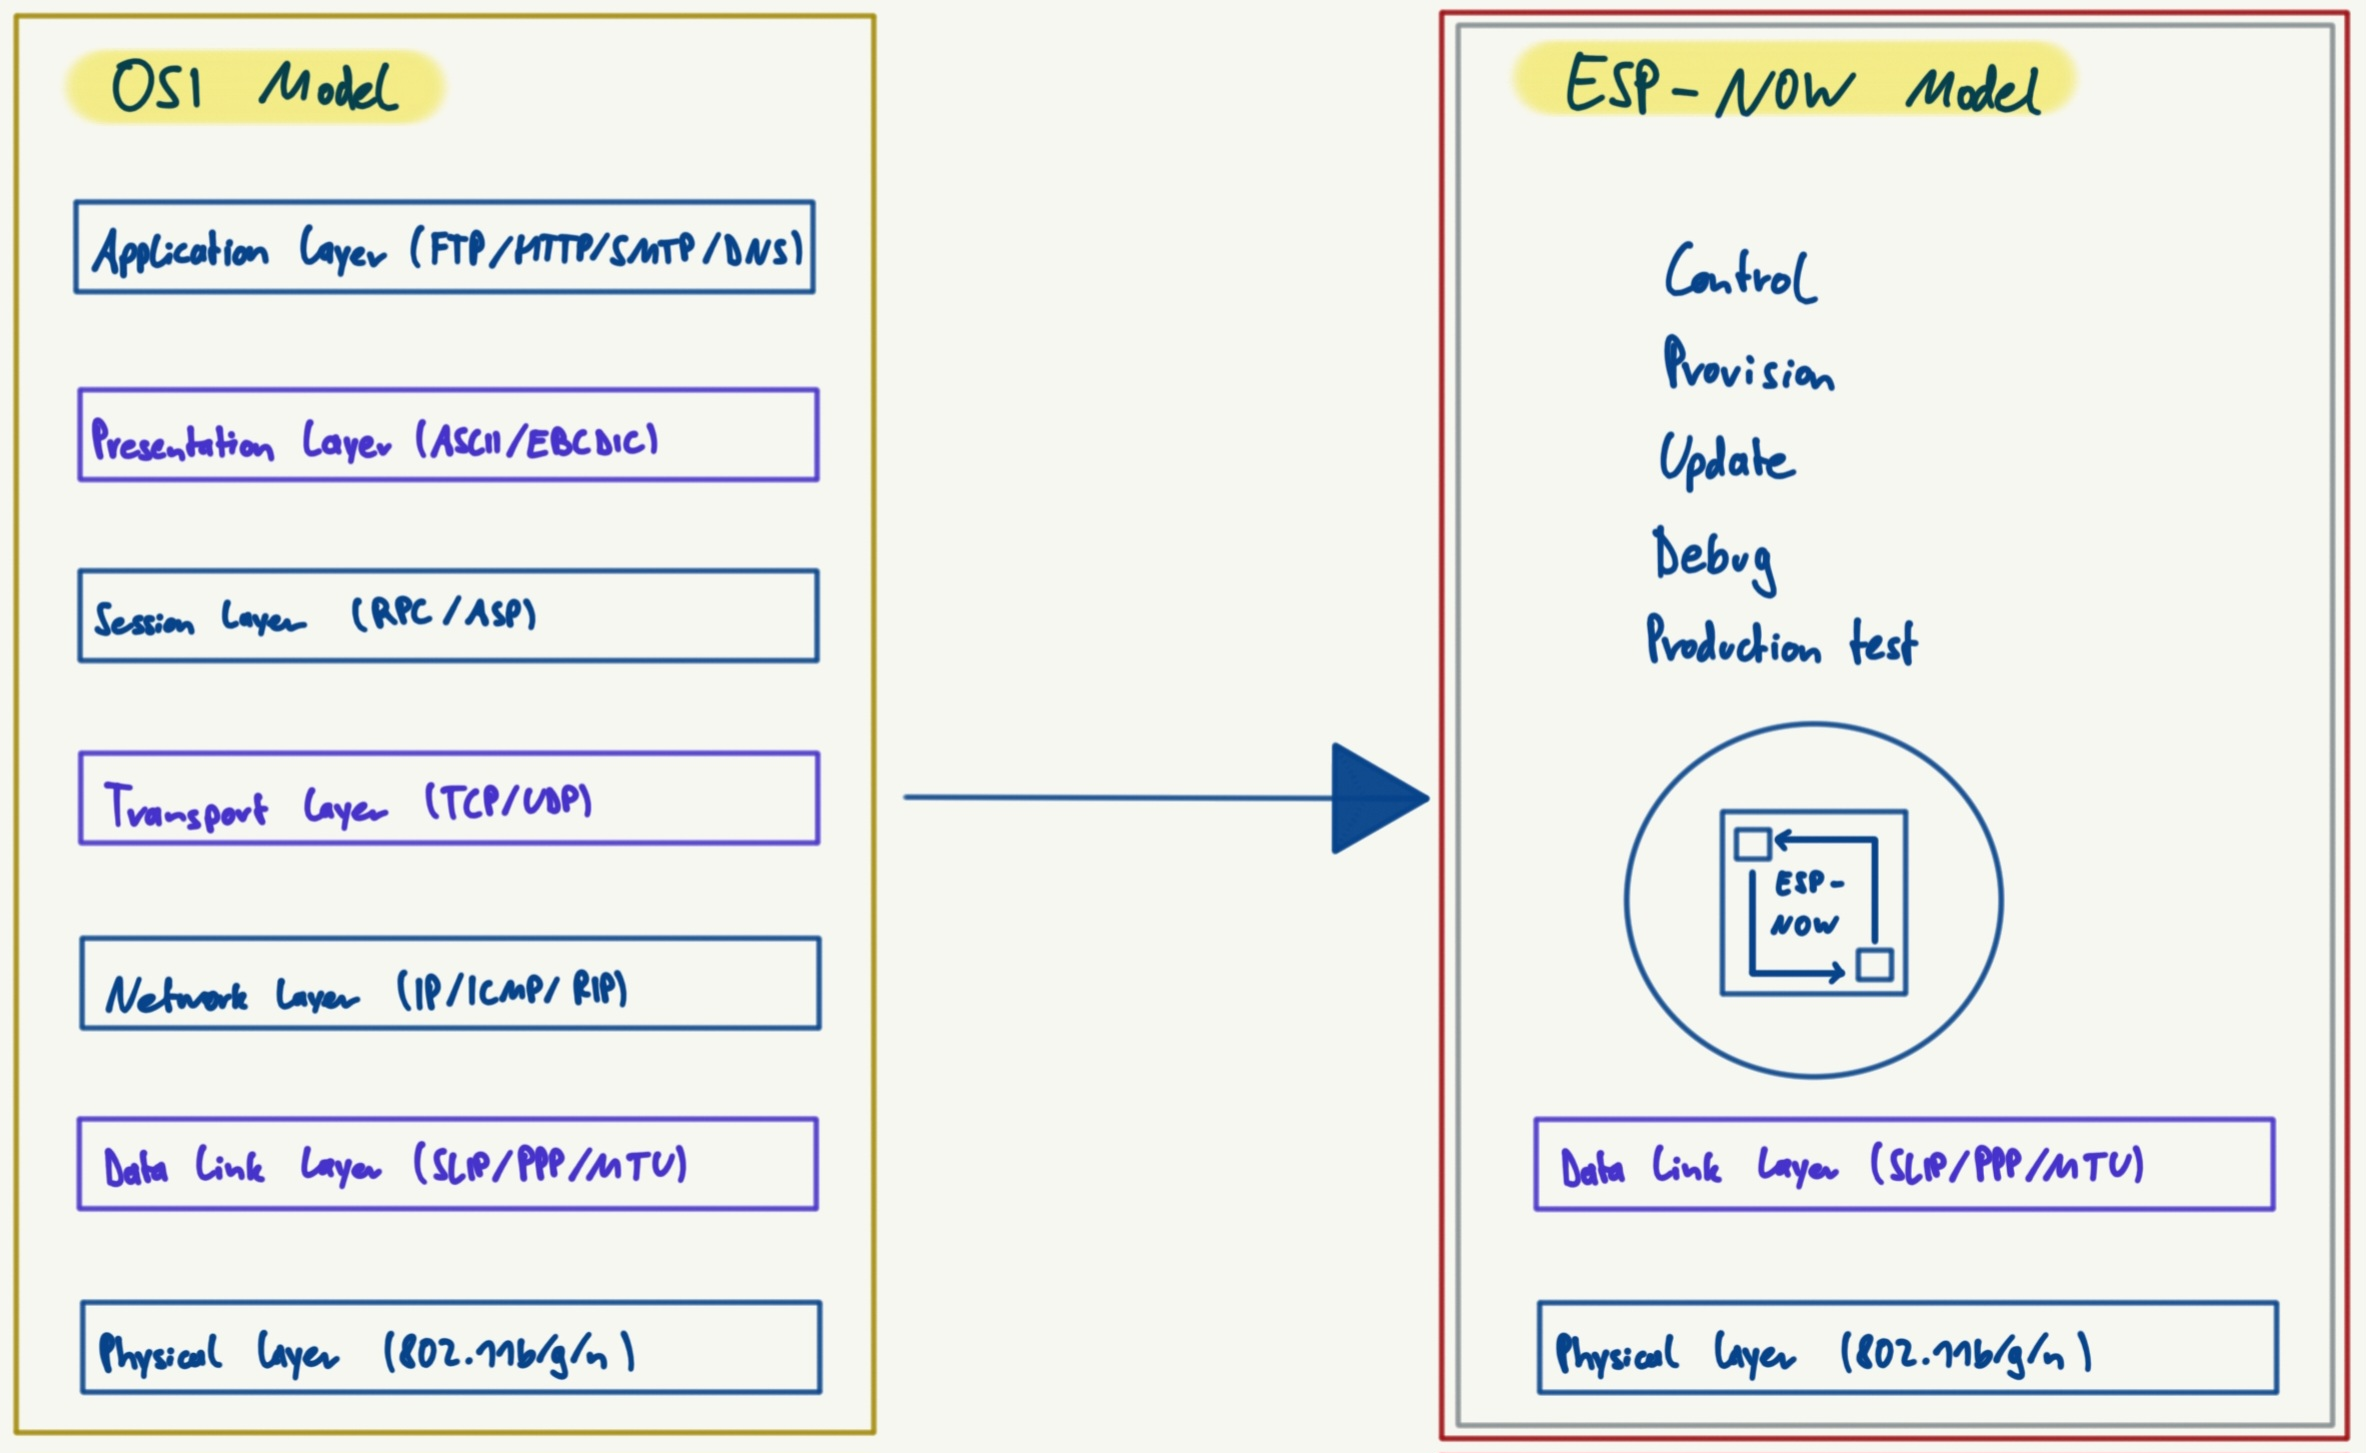
\includegraphics[width=0.8 \linewidth]{ESPNOW_Model}}
		%\caption*{Ladislaus Szabo}
	\end{center}
\end{figure}

\subsubsection{OSI-Modell}
Das OSI-Modell ist standardisiert und ermöglicht die Kommunikation zwischen den 
verschiedensten Computersystemen. OSI (Open Systems Interconnection) wurde von der 
ISO (International Organization for Standardization) erfunden. 
Es besteht aus 7 Schichten (application layer, presentation layer, session layer, 
transport layer, network layer, data link layer und physical layer). Wichtig ist, 
dass jede einzelne Schichte eine andere Aufgabe erfüllt. Durch das System der 
einzelnen Schichten kann die Fehlersuche vereinfacht werden, da man die jeweiligen 
durchforsten kann. Zu beachten ist allerdings, dass diese untereinander ebenfalls 
Daten austauschen und untereinander kommunizieren können. Dabei ist jede Schicht 
nach international standardisierten Protokollen definiert. Das bedeutet, das gewisse 
Regeln zur Kommunikation eingehalten werden müssen. Dabei ist es möglich, dass sich 
ein Protokoll über mehrere Schichten verteilt. \\
\\
Beim Sender und Empfänger werden diese sieben Schichten jeweils einmal angewandt. \\
\\

\paragraph{Physical Layer}
\hfill \break
\hfill \break
Beschreibt die mechanische und funktionale Schnittstelle zum Übertragungsmedium. Die 
Datenübertragung der physischen Geräte, wie Schalter, Kabel, usw. ist hiermit gemeint. 
Daten werden in einen Bitstrom umgewandelt. Zu beachten ist, dass das Übertragungsmedium 
an sich nicht zur 1. Schicht gehört, nur die Datenübertragung bei Einschalten des 
physischen Geräts gehört in diese.\\

\paragraph{Data Link Layer}
\hfill \break
\hfill \break
Beschreibt die Sicherungsschicht, die eine stabile und funktionierende Verbindung 
zwischen Endgerät und Übertragungsmedium herstellt. Der Data Link Layer verarbeitet 
Pakete vom Network Layer, spaltet diese in kleinere Teile namens Frames und ist für 
den Datentransfer zwischen zwei Geräten im selben Netzwerk verantwortlich. Die 
physikalische Adressierung von Datenpaketen wird hier durchgeführt. Außerdem werden 
auch eine Fehlererkennung, Fehlerbehebung und Datenflusskontrolle angewandt. \\

\paragraph{Network Layer}
\hfill \break
\hfill \break
Beschreibt den regulierten Datentransfer zwischen zwei verschiedenen Netzwerken. Hier 
werden einzelne Segmente auf dem Sendergerät von dem Transport Layer in Fragmente 
aufgeteilt und auf dem Empfängergerät dann wieder zusammengefügt. Die logische Adressierung 
findet ebenfalls statt. \\

\paragraph{Transport Layer}
\hfill \break
\hfill \break
Beschreibt das Bindeglied zwischen den transportorientierten und den anwendungsorientierten 
Schichten. Wie immer, werden die Daten in kleinere Bestandteile zerlegt. Header-Informationen 
und eine Fehlerkontrolle werden von den Segmenten beinhaltet, falls nicht alle Daten 
erfolgreich angekommen sind oder fallengelassen wurden, kann dies hilfreich sein. \\

\paragraph{Session Layer}
\hfill \break
\hfill \break
Beschreibt die Verbindung zwischen den Endsystemen. Session nennt man den zeitlichen 
Bereich zwischen dem Starten und Beenden der Kommunikation. Wichtig ist auch, dass 
dieser Layer dafür verantwortlich ist, dass genug lange Daten übertragen werden können 
und die Verbindung nicht schon zuvor beendet wird. Für die Effizienz soll allerdings 
nach einem abgeschlossenen Vorgang die Verbindung unterbrochen werden. \\

\paragraph{Presentation Layer}
\hfill \break
\hfill \break
Beschreibt die Aufbereitung der Daten, sodass der Nutzer diese verstehen kann. Damit 
ist gemeint, dass beispielsweise verschlüsselte Daten zuerst entschlüsselt werden 
müssen, bevor sie der Nutzer verstehen kann. Die Komprimierung und Dekomprimierung 
von Daten werden hier auch durchgeführt. \\

\paragraph{Application Layer}
\hfill \break
\hfill \break
Beschreibt die Bereitstellung von Funktionen für Anwendungen und die Verbindung zu 
den unteren Schichten. Die Dateneingabe und Datenausgabe werden hier ebenfalls 
durchgeführt. Softwareanwendungen sind auf den Application Layer angewiesen (http, SMTP, …). 
Diese Protokolle sind für die Kommunikation notwendig und standardisiert. \\

\paragraph{ESP-NOW Schichten}
\hfill \break
\hfill \break
Es gibt bei ESP-NOW zwei Schichten, den Data Link Layer und den Physical Layer 
(siehe OSI-Modell). Dabei beruht der Physical Layer auf dem IEEE 802.15.4 Standard. 
Da jedoch nicht so viele Schichten, wie bei dem OSI-Modell vorhanden sind, gibt es 
mehrere Möglichkeiten, wo Fehler liegen können und es ist nicht so leicht den Fehler 
an der richtigen Stelle zu suchen. \\

\paragraph{IEEE 802.15.4 Standard}
\hfill \break
\hfill \break
Es ist ein internationaler Standard für die drahtlose Kommunikation, der von 
Electrical and Electronics Engineers (IEEE) entwickelt wurde. Besonders wird Wert auf 
die geringe Datenrate und dem daraus folgend geringen Stromverbrauch Wert gelegt. Es 
werden lizenzfreie Frequenzbänder im 2,4GHz-, 915MHz- und 868MHz-Bereich verwendet. \\
\\
\begin{figure}[H]
	\begin{center}
		\scalebox{0.8}
		{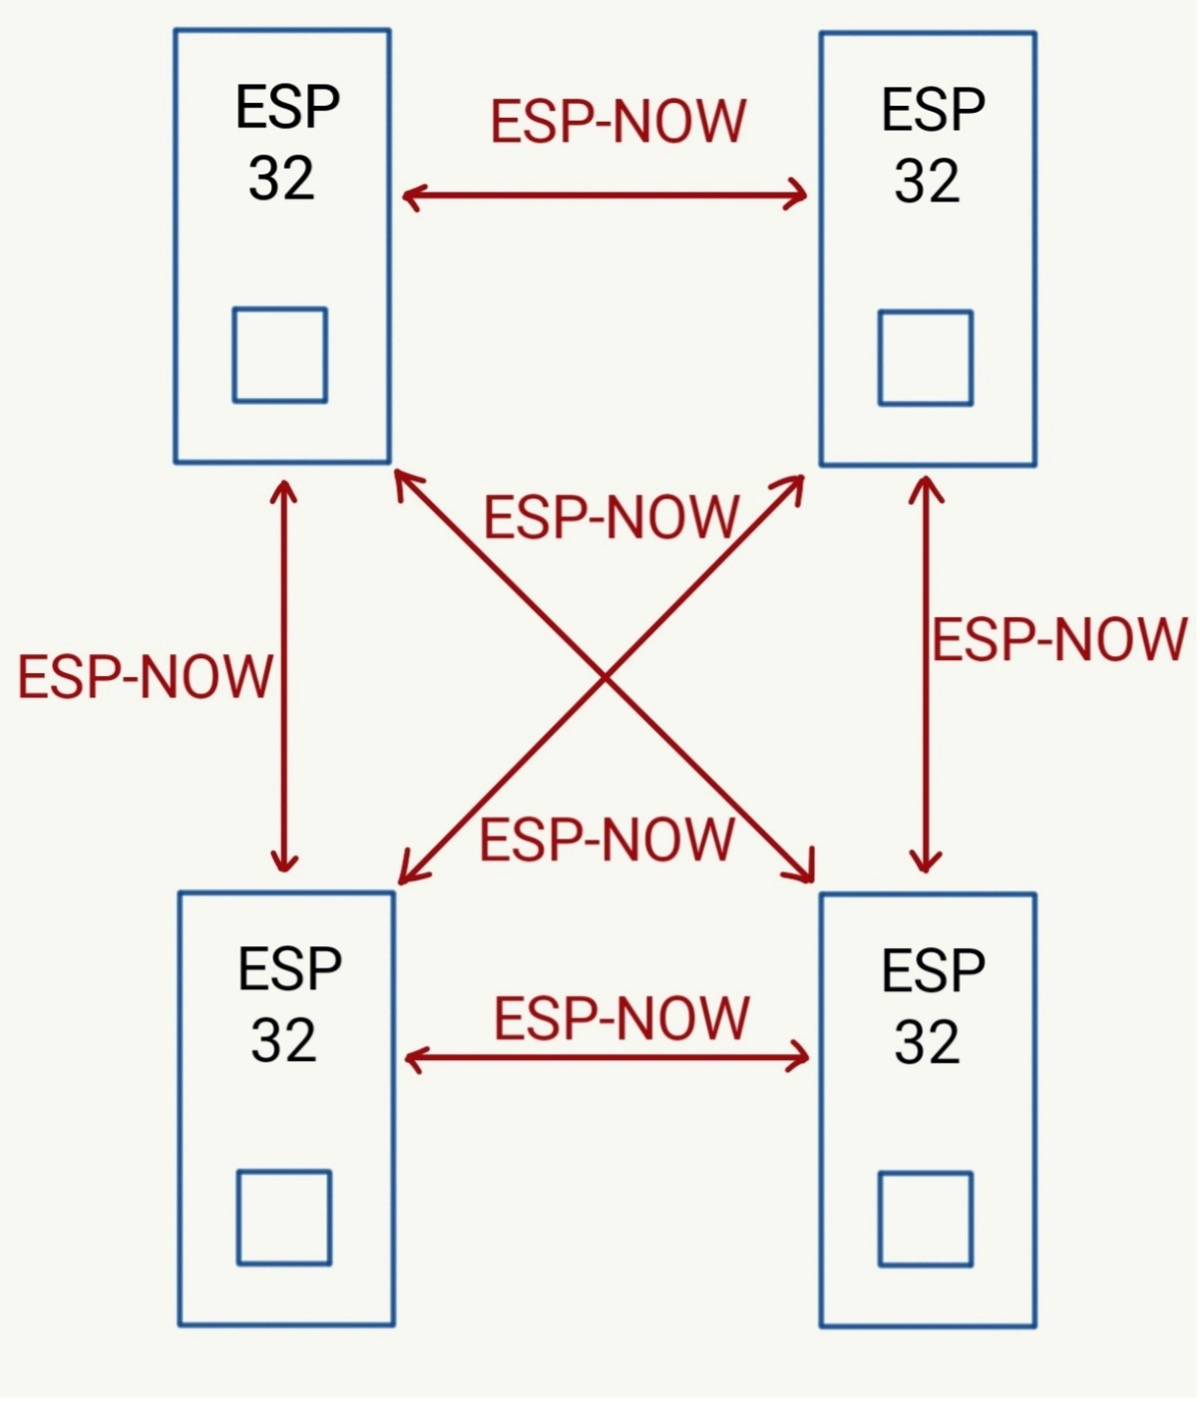
\includegraphics[width=0.8 \linewidth]{ESP_NOW_Theorie}}
		%\caption*{Ladislaus Szabo}
	\end{center}
\end{figure}
\hfill \break

\subsection{OPV Technologien \textcolor{red}{Laci}}
Ein Operationsverstärker, kurz OPV, ist ein analoger Gleichspannungsverstärker, der sich durch seine üblicherweise sehr hohe 
Verstärkung auszeichnet. Der elektroische Grundbaustein ist ein Differenzverstärker, der durch äußere Beschaltungen angepasst werden kann.
In der grundlegendsten Funktion, verstärkt ein OPV die Differenz der beiden Eingangsspannungen am $"$+$"$ und $"$-$"$ Anschluss. Das Ergebnis
dieses Verstärkungsprozesses wird anschließend über $"$Vout$"$ ausgegeben. \\
\\
Operationsverstärker können mit einem sogenannten $"$Single-Supply$"$ oder $"$Dual-Supply$"$ versorgt werden. Dies bezieht sich auf
die Art der Versorgungsspannung. \\
\\
\subsubsection{Single-Supply}
Bei dieser Art der Versorgung, wird ausschließlich eine positive Spannung und das Groundpotential genutzt. Das bedeutet, dass der OPV
theoretisch einen maximalen Ausgangsbereich von GND bis VCC haben kann. Negative Spannungen können nicht ausgegeben werden. \\
\\

\subsubsection{Dual-Supply}
Beim Dual-Supply Betrieb, wird der OPV von einer positiven und negativen Spannung versorgt. Das bedeutet, dass der OPV nun die Fähigkeit
besitzt auch negative Spannungen auszugeben und der Ausgangsspannungsbereich somit größer als beim Single-Supply ist.

\subsubsection{Rail-to-Rail Technologie}
Hat ein OPV die sogenannte $"$Rail-to-Rail Technologie$"$, so ist die Rede von Spannweite des Ausgangsspannungsbereichs. Bei diesem Feature
ist der Operationsverstärker dazu fähig fast bis auf das positive und negative Versorgungspotential Spannung auszugeben. Dies ist oft 
von Vorteil, da dadurch die Versorgungsspannungen nicht übermäßig hoch sind und somit die Schaltungen mit niedrigeren Spannungen arbeiten
kann. Dies ist auch für die Benutzer der entsprechenden Endgeräte sicherer.\\
\\
In der folgenden Grafik sind die Ausgangsspannungsbereiche eines normalen OPVs, in blau, und eines OPVs mit Rail-to-Rail Technologie,
in Orange, dargestellt. \\
\begin{figure}[H]
	\begin{center}
		\scalebox{1.2}
		{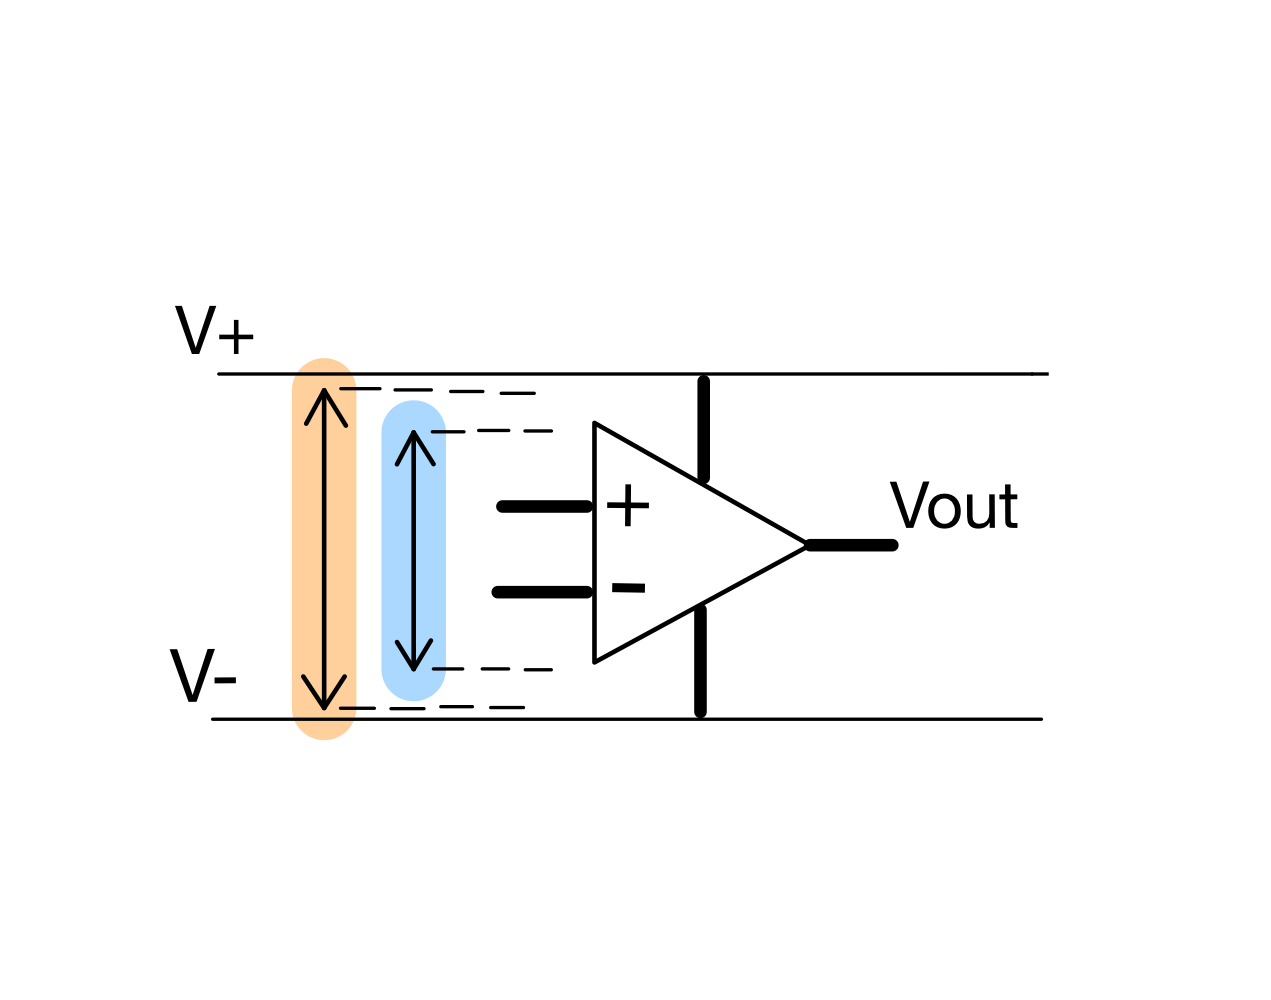
\includegraphics[width=0.8 \linewidth]{RAILtoRAIL_OPV}}
		%\caption*{Ladislaus Szabo}
	\end{center}
\end{figure}

\subsection{PWM-Signale}

%--------------------------------------------------------------------------
%--------------------------------------------------------------------------

\section{Grundlegende Systemkonzepte}

\subsection{Gesamtsystemkonzept}

\subsubsection{Systembeschreibung}

	\begin{figure}[H]
		\begin{center}
			\scalebox{1.2}
			{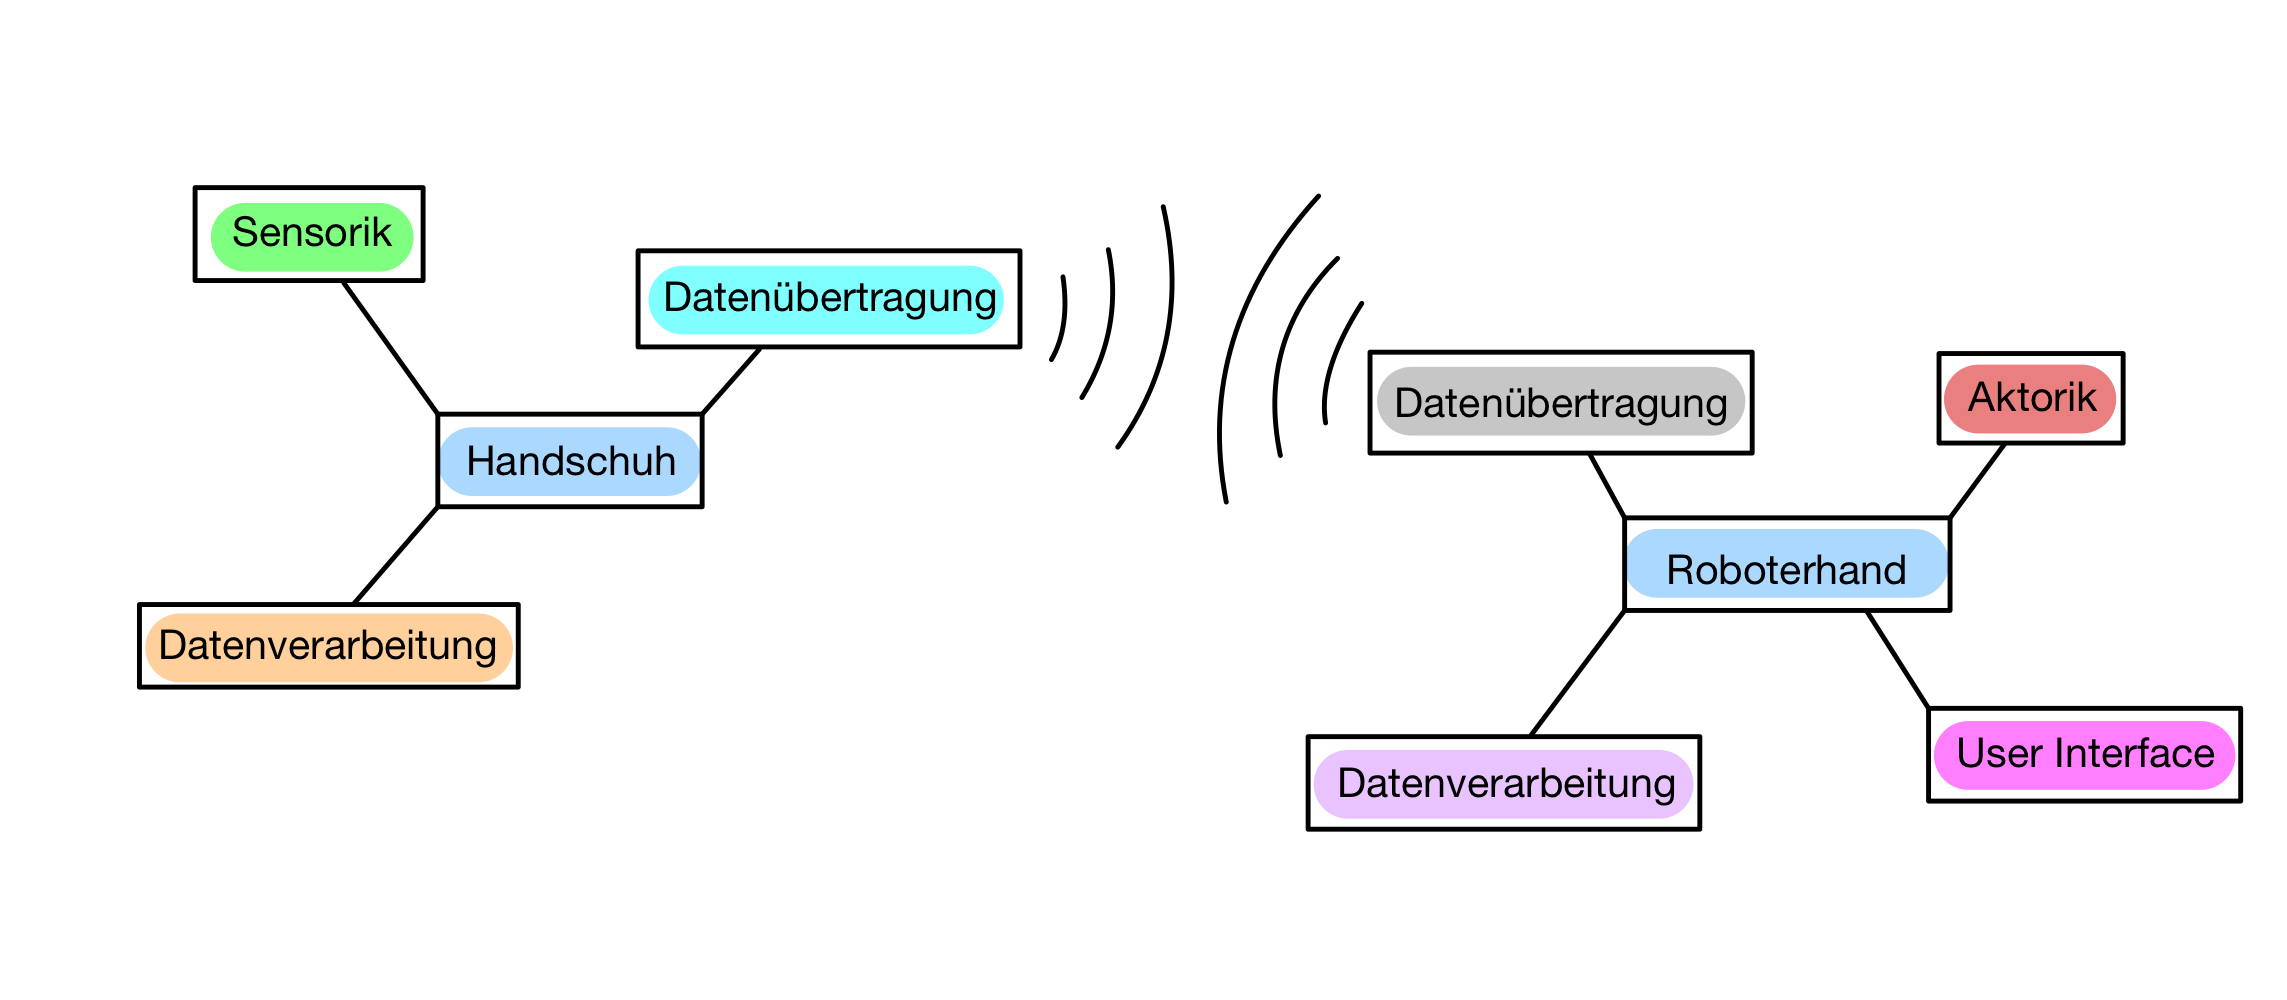
\includegraphics[width=0.8 \linewidth]{Blockschaltbild_Gesamtsystem}}
			%\caption*{Ladislaus Szabo}
		\end{center}
	\end{figure}

Das Gesamtsystem ist im oberhalb abgebildeten Blockschaltbild grafisch veranschaulicht. Die linke Hälfte zeigt das Konzept des 
Handschuhs (Eingabe) und die rechte Hälfte die Roboterhand (Ausgabe). Die grundlegende Konzeptionierung der Bewegungserfassung 
besteht darin, dass mithilfe von Sensoren die Fingerbeugung aller fünf Finger gemessen wird. Anschließend werden die Sensordaten
ausgewertet und verarbeitet. Die resultierenden Informationen werden folglich über eine drahtlose Verbindung an das zweite 
Subsystem, nämlich der Roboterhand, übertragen. Dort wird das Gesendete empfangen, weiterverarbeitet und interpretiert. Die Aktorik
setzt die digitalen Anweisungen in mechanische Bewegungen um, wodurch die Roboterhand gesteuert wird. Im Ausgabesystem ist auch 
ein User-Interface enthalten. Die diversen Funktionen werden in späteren Punkten näher erläutert.

\subsection{Eingabesubsystem}

	\begin{figure}[H]
		\begin{center}
			\scalebox{0.8}
			{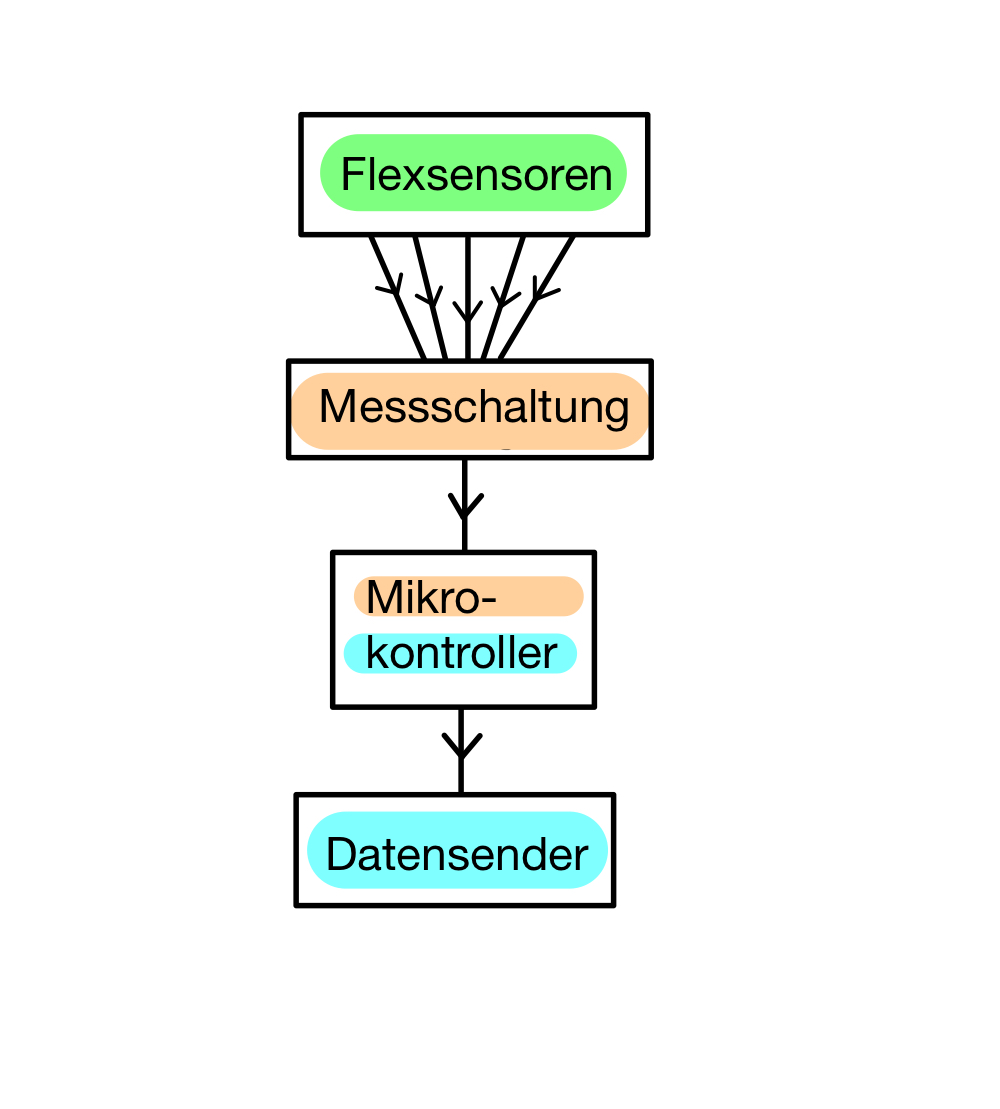
\includegraphics[width=0.8 \linewidth]{Blockschaltbild_Handschuhsystem}}
			%\caption*{Ladislaus Szabo}
		\end{center}
	\end{figure}

Der Sensorhandschuh ermöglicht dem Benutzer die Roboterhand zu steuern. Dies geschieht durch Flexsensoren, die an den Fingern des 
Handschuhs angebracht sind. Wird ein Finger gebeugt, so ändert sich ich der Widerstandswert der korrespondierenden Sensoren. Diese Änderungen 
werden von einer Messschaltung erfasst, die die Sensorwerte interpretiert, digitalisiert und anschließlich an den Mikrokontroller über ein 
Kommunikationsprotokoll weitergibt. \\

\subsection{Ausgabesubsystem}

\begin{figure}[H]
	\begin{center}
		\scalebox{0.8}
		{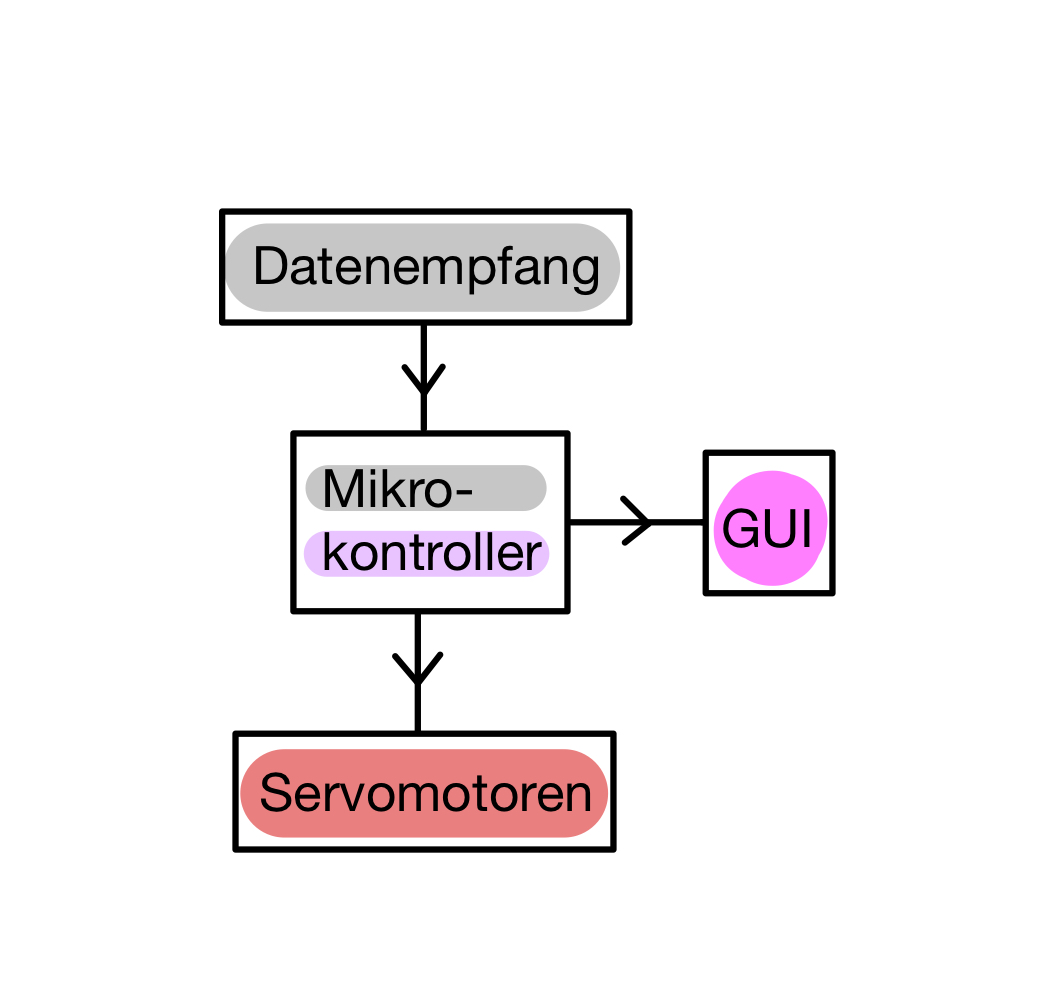
\includegraphics[width=0.8 \linewidth]{Blockschaltbild_Roboterhandsystem}}
		%\caption*{Ladislaus Szabo}
	\end{center}
\end{figure}

Sind die Daten des Eingabesubsystems empfangen, müssen diese in ein geeignetes Format für die Steuerung der Aktorik, also den Servomotoren,
umgewandelt werden. Dies geschieht mit dem Mikrokontroller. Angebunden an das Ausgabesubsystem ist ein Graphical-User-Interface, 
weclhes in Punkt 8.3 näher erklrärt wird. \\

%--------------------------------------------------------------------------
%--------------------------------------------------------------------------

\section{Mechanische Realisierung}

\subsection{Handschuh \textcolor{red}{Amir}}
\subsubsection{\textcolor{purple}{Platzhalter für diverse Unterpunkte von Amir}}

\subsection{Roboterhand \textcolor{red}{Amir}}
\subsubsection{Der Grundgedanke}
Der Grundgedanke der Mechanik in der Roboterhand ist es alle drei Glieder eines Fingers,
darunter das Fingergrundglied, das Fingermittelglied und das Fingerendglied mit 
ausschließlich der Bewegung eines einzelnen Servomotors auf oder zu zuklappen. 
Umsetzbar ist dies durch ein Zugsystem, welches für ein Aufklappen und ein Zuklappen 
des Fingers ermöglicht. Gezogen wird durch den Finger der Roboterhand ein oder mehrere 
Schnüre, ähnlich wie bei einer Marionette. Diese Schnüre bringen den Finger je nach 
Verlängern oder Verkürzen zum Bewegen. Ebenso ist je nach Zug wählbar in welcher 
Stellung der Finger sich dann befindet. Befestigt wird dies an einem mit dem Servomotor 
gesteuertem Zugmechanismus. \\

\paragraph{Fertigung und CAD}
\hfill \break
\hfill \break
Der Entwurf eines Modells ist mit ständiger Weiterentwicklung verbunden, sind in 
solch einem Modell mechanische Komponenten vorhanden nimmt die Fertigungsschleife 
ersichtlich mehr Komplexität an und erfordert die Möglichkeit in kürzester Zeit 
flexibel Anpassungen und Optimierungen am Entwurf ausgiebig zu testen. Speziell 
während der Entwicklung der mechanischen Komponente einer Roboterhand ist auf 
viele Faktoren zu achten, es ergeben sich ständig neue Erkenntnisse sowie auch 
Problematiken, welche eine Lösung erfordern. Sei es mangelnde Stabilität unter 
hoher Belastung, zu viel Reibung oder gängige Konstruktionsfehler. \\
\\
Dank dem neuen Fertigungsverfahren des 3D-Drucks ist es möglich Versuchsaufbauten 
in einem CAD-Programm zu entwerfen, diese folglich zu drucken und dementsprechend 
auf ihr Verhalten zu testen. \\
\\
Ein CAD-Programm ist eine Software, welche zur Erstellung von zweidimensionalen 
oder auch dreidimensionalen Komponenten Modellen dient, CAD steht für Computer-Aided 
Design(engl.) und bedeutet übersetzt „Computerunterstütztes Entwerfen“. Neben 
dem reinen Entwerfen von Modellen haben solche Programme auch die Eigenschaft, 
das Modell je nach Material auf Stabilität, maximal Belastung oder sonstige 
Verhaltensmuster zu testen. \\
\\
Das 3D-Verfahren arbeitet mit den exportierten Modell-Dateien eines CAD-Programms 
und setzt diese in ein greifbares Modell um. \\
Dabei gibt es darunter mehrere Fertigungsmethoden, die von uns gewählte ist die 
gängigste, FDM (Fused Deposition Modeling), dieses Verfahren arbeitet hauptsächlich 
mit Kunststoffen. Dabei zeichnet ein Extruder mit eingeführtem Filament Sichtweise 
ein Modell auf eine Druckplatte und formt damit ein reales Objekt. Kunststoffe, 
die für dieses Fertigungsverfahren verwendet werden ist PLA, ABS, PETG und weitere. \\
Die Vorteile des FDM-Drucks sind, dass die Druckgeräte sowie das Filament billig 
zu erhalten sind. Aber auch die das Verfahren einfach und nicht besonders komplex 
ist, sowie auch schnell. \\

\textcolor{red}{(Quelle: Zum zitieren und Quellenverzeichnis: https://filamentworld.de/3d-druckverfahren/)}

\subsubsection{Versuchsaufbauten}
In diesem Versuchsaufbau war es das Ziel mit einem simplen Testmodell Erkenntnisse über 
den Mechanismus zu erhalten und dadurch mehr aus ihm zu lernen. 
Dafür wurde in der CAD Software Fusion360 ein erstes Testmodell entworfen. \\

\paragraph{Aufbau}
\hfill \break
\hfill \break
Das Modell besteht aus den drei Gliedern eines Fingers, einer Halterung für einen 
Servomotor, sowie aus den im Inneren vorhandenen Führungen. \\
\\
Zwischen jedem Fingerglied befindet sich 1cm Abstand, verbunden sind diese durch eine 
3mm dicke Fläche. Die Fläche hat den Zweck sich bei Zug an der Schnur zu biegen, durch 
die Führungen wird nur eine Biegung an der „Fläche“ ermöglicht. Befestigt wird die
Schnur an einer Halterung am Servomotor und wir dadurch bei Rotation des Servos 
entsprechend angezogen. Die Fingerglieder haben eine nach außen gewölbter Form und sind 
in Richtung der Fläche verjüngt, dies ermöglicht dem Finger sich auf noch engeren Raum 
zusammenzuziehen.

\paragraph{Versuchsresultat}
\hfill \break
\hfill \break
Das Versuchsresultat war nahrhaft und bot einen breiten Einblick in den Mechanismus. 
Dabei gab es zahlreiche Erkenntnisse über Reibung, Stabilität und mechanische Abnutzung 
sowie aber auch Belastung. \\
\\
Einer der Erkenntnisse war es, dass die Schnur eine gewisse Zugfestigkeit benötigt. 
Getestet wurden dabei mehrere Schnüre unter anderem auch Nylonschnüre. Als besonders 
stabil haben sich dann Angelschnüre bewiesen.
Festgestellt wurde ebenso, dass ein mechanischer Widerstand benötigt wird, welcher den 
Finger wieder in seine Ursprungsposition: ausgestreckt – versetzt. Anfangs war dafür 
die freie Fläche vorgesehen, diese hat sich jedoch über die Zeit abgenutzt und hat den 
Finger nicht in die Ursprungsposition befördert. Eine mögliche Lösung während 
Gummikordeln, elastische Schnüre, welche am „Fingerrücken“ platziert werden und sich 
bei Biegen des Fingers spannen. Desto kürzer die Zugschnur im Finger, desto länger die 
Gummikordel. \\

\subsubsection{Erste Testhand}
\paragraph{Konzept Einführung}
\hfill \break
\hfill \break
Die erste Testhand zielt darauf ab ein Modell welches durchgängig erweitert 
werden kann zu schaffen. Mit Rücksicht auf etwaige Testergebnisse des 
Versuchsresultats (Verweis auf 6.2.1.2) soll ein Modell geschaffen werden, 
welches den im Versuch aufgetretenen Problematiken entgegenwirkt. Unter anderem 
der nicht vorhandene Rückzug, eine Schnur für den Zug mit ausreichender 
Reißfestigkeit sowie eine anwendungsgemäße Konstruktion des Fingers. \\
\\
Eine konkrete Lösung, um für mehr Sicherheit im Zusammenhang mit dem Zugsystem 
zu sorgen wurde für diesen Aufbau eine Angelschnur mit einem Durchmesser von 
XXmm gewählt, diese hat eine Kraft von XX/m. Aufgrund der XXX ist die Schnur 
ebenso schnittfest. \\
\\
Im Versuch (Verweis) hat sich erwiesen, dass eine Fläche aus PLA welche die 
Fingerglieder verbindet nicht genügend Kraft aufbringt, um den Finger wieder in 
seine Ursprungsposition zu bewegen. Demnach wird eine Kraft benötigt, welche 
ständig dem Zug der Angelschnur entgegenwirkt und den Finger entsprechend 
austreckt. \\
In diesem Modell wird daher ein Elastomer, ein elastisches Material in Form 
eines Bandes mit ausreichender Kraft gewählt. \\

\paragraph{Mechanismus}
\hfill \break
\hfill \break

\paragraph{Realisierung und Zusammenbau}
\hfill \break
\hfill \break

\paragraph{Fazit und Ergebnisse}
\hfill \break
\hfill \break

\subsubsection{Zweite Testhand (Inmoov)}
\paragraph{Einführung}
\hfill \break
\hfill \break

\paragraph{Realisierung und Zusammenbau}
\hfill \break
\hfill \break

\paragraph{Fazit und Ergebnisse}
\hfill \break
\hfill \break

\subsubsection{Drite Testhand (Projekt-Silikonhand)}
\paragraph{Konzepterläuterung}
\hfill \break
\hfill \break

\paragraph{Erste Versuche einer Gussform und Asuwertung}
\hfill \break
\hfill \break

\paragraph{Verbesserungen und Realisierung (Gelenke im Guss)}
\hfill \break
\hfill \break

\paragraph{Verbesserung der Gelenke}
\hfill \break
\hfill \break

\paragraph{Entwurf einer neuen Gussform}
\hfill \break
\hfill \break

\paragraph{Vorbereitung und Probleme beim Guss}
\hfill \break
\hfill \break

\paragraph{Konzeptverbesserung}
\hfill \break
\hfill \break

\paragraph{Fazit und Stellungnahme (Konzept verworfen)}
\hfill \break
\hfill \break

\subsubsection{Vierte Hand}
\paragraph{Erfahrung und Konzepterläuterung}
\hfill \break
\hfill \break

\paragraph{Erster Entwurf}
\hfill \break
\hfill \break

\paragraph{Verbesserungen – zweiter Entwurf}
\hfill \break
\hfill \break

\paragraph{Realisierung und Aufbau}
\hfill \break
\hfill \break

\paragraph{Versuche...}
\hfill \break
\hfill \break

%--------------------------------------------------------------------------
%--------------------------------------------------------------------------

\section{Hardware Realisierung}

\subsection{Eingabesubsystem}

\subsubsection{Grundlegende Voraussetzungen \textcolor{red}{Laci}}
Die Hardware des Eingabesubsystems muss einige Kriterien erfüllen, um schlussendlich voll funktionfähig in das Gesamtsystem eingebaut 
werden zu können. Zunächst ist die Größe der Schaltung, als mit der wichtigste Punkt zu nennen. Da es bei diesem Projekt nicht nur
um die Funktionalität, sondern auch um ein ergonomisches Benutzererlebnis geht, sollte die entgültige Platine auf dem Handschuhrücken
nicht größer als 4cm x 4cm sein. Beim Design der Elektronik muss durch die Größenrestriktion natürlich darauf geachtet, dass durch
diese keine Einbußen in Bezug auf die korrekte und sichere Funktion des Projektteils entstehen. Übermäßige Wärmeentwicklung ist 
ebenfalls zu vermeiden, da diese auf lange Zeit unangenehm für den Endnutzer ist. Die Versorgung der Schaltung
sollte möglichst über einen kleinen und portablen Akku geschehen, um dem Benutzer das bestmögliche Erlebnis zu bereiten. Dieses Feature ist
allerdings optional und ist daher nicht garantiert zur Verwendung bereit. Über einen USB Anschluss soll der Mirkokontroller programmierbar sein und die Schaltung
auch für Test -und Wartungszwecke versorgt werden können. Das Maximalgewicht darf 500g nicht übersteigen. \\

\subsubsection{Überlegungen, Simulationen und Berechnungen \textcolor{red}{Laci}}
\paragraph{Bewegungserfassung der Fingerbeugung}
\hfill \break
\hfill \break
Die Bewegungen des Benutzers müssen gemessen werden können. Das bedeutet, dass eine Form von Messschaltung notwendig ist um die  
Beugung der Finger interpretieren zu können. Dies könnte man durch das Messen des Beugungswinkels realisieren. Allerdings hat 
jeder Finger drei Gelenke, wodurch man diese auch bei der Roboterhand individuell steuern müsste. Die zweite Möglichkeit wäre, 
durch eine visuelle Aufnahme die Bewegung des Handschuhs und dadurch des Benutzers aufzuzeichnen. Da dies allerdings nur in dafür vorgesehenen, 
mit Kameras ausgestatteten, Räumen funktionieren würde, ist dies für uns auch keine sinnvolle Möglichkeit. Schließlich haben 
wir uns für die Erfassung der Fingerbewegungen mittels Flexsensoren entschieden. Diese ändern den Widerstand je nach der 
aktuell vorherrschenden Beugung. Bei dieser Art der Bewegungserfassung muss man nicht jedes Fingergelenk einzeln steuern und 
braucht auch keine externen Kameras. Somit ist bei dieser Methode der Datenerfassung ein sehr flexibler Verwendungsbereich 
des Handschuhs gewährleistet. Um die Änderungen der Widerstandsstreifen messen und verarbeiten zu können ist nun eine Schaltung 
notwendig. Diese muss Wertdifferenzen erkennen und in ein geeignetes Format zur Weiterverarbeitung mit einem Mikrokontroller
umwandeln können.
\\
\\
\paragraph{Auslesen der Sensoren}
\hfill \break
\hfill \break
Das Auslesen der Flexsensoren kann durch einen einfachen Spannungsteiler erfolgen. Dabei ist die Genauigkeit
allerdings nicht optimal und ist daher nicht für unsere Anwendung geeignet. Als Lösung für dieses Problem haben wir an eine 
OPV-Messschaltung gedacht. Diese soll mit einem Shuntwiderstand die Spannungsdifferenz messen, die sich bei einer Veränderung 
des flexiblen Widerstands ergibt. Durch eine geeignete Verstärkung des OPVs kann diese mit einer Referenzspannung verglichen 
werden. \\
\begin{figure}[H]
	\begin{center}
		\scalebox{1.25}
		{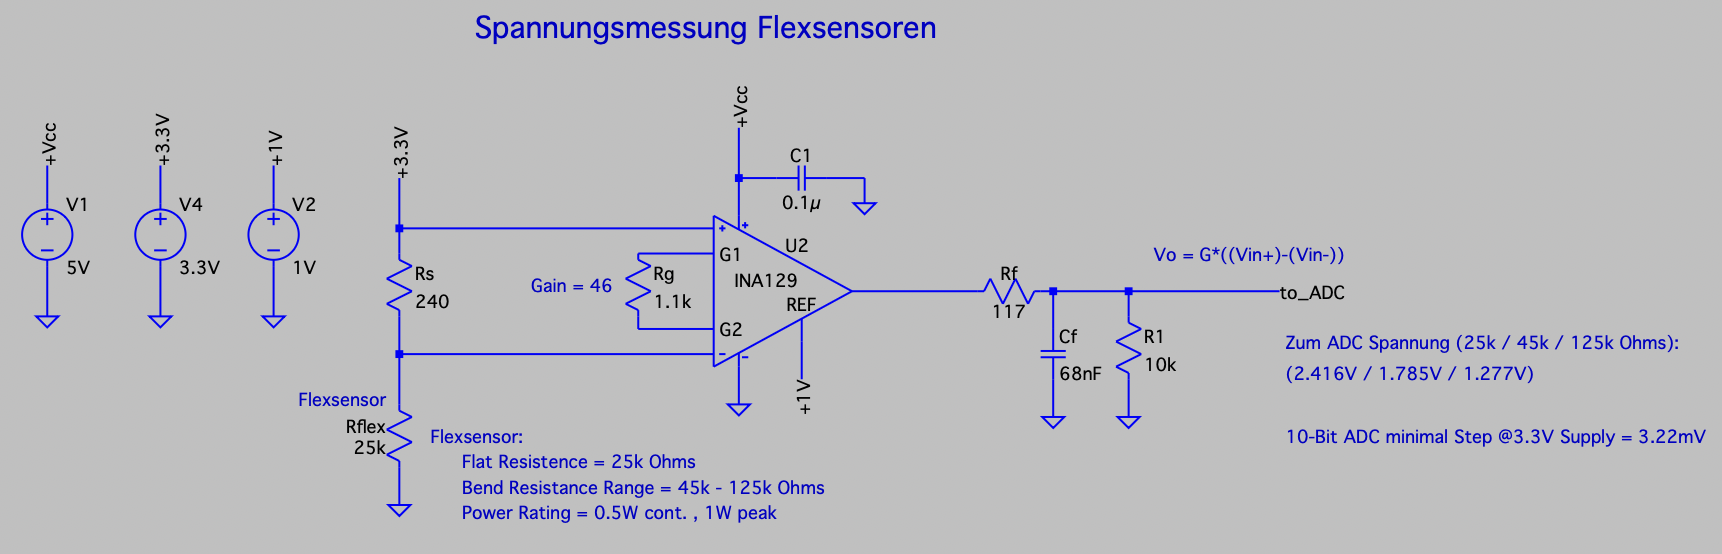
\includegraphics[width=0.8 \linewidth]{Simulation_Spannungsmessung_Flexsensoren}}
		%\caption*{Ladislaus Szabo}
	\end{center}
\end{figure}
\hfill \break
Die Flexsensoren (Rflex) beziehen ihre Versorgung über einen Shunt-Widerstand (Rs). Je nach Belastung, ändert sich der 
Spannungsabfall an diesem (Je größer die Beugung des Sensors, desto kleiner ist der Spannungsabfall). Die Spannungsdifferenz 
am Shunt-Widerstand wird von einem Operationsverstärker verstärkt. Bei der Auswahl des OPVs sind einige Punkte zu beachten, um 
eine korrerkte und genaue Erfassung der Fingerbeugung zu gewährleisten. \\
\\
Folgende Kriterien müssen folglich bei der Wahl des Operationsverstärkers beachtet werden:
\begin{itemize}
	\item Ausgangspegel bei gewählter Versorgungsspannung: \\
		  \\
		  Zunächst wurde das Kriterium der Versorgungsspannung betrachtet. Da wir maximal 5V Gleichspannung in der gesamten 
		  Schaltung verwenden wollen, muss der OPV mit dieser geringen Spannung immer noch verstärken. Da am positiven 
		  Verstärkereingang eine maximale Spannung von 3.3V anliegt, muss dies bei Verstärkern mit einer geeigneten Supply Range 
		  auch mit nur 5V Versorgungsspannung gewährleistet sein.
	\item Referenzspannung: \\
		  \\
		  Ein weiteres Kriterium ist das vorhanden sein eines Referenzspannungsanschlusses. Da der OPV keine Rail-to-Rail 
		  Technologie besitzt, muss der Ausgangsspannungspegel auf ein gewisses minimum angehoben werden. In unserem ist dies 
		  +1V. Würde diese Refernzspannung nicht vorhanden sein, so würde der OPV falsche Werte erzeugen, da dieser erst ab einer
		  verstärkten Spannung am Ausgang von ca. 750mV korrekt funktioniert.

\end{itemize}
Aufgrund dieser Kriterien und der Notwendigkeit von Genauigkeit und geringer Störungseigenschaften, viel die Wahl des 
Operationsverstärkers auf den INA129 instrumentation amplifier. \\
\\
Der Shunt-Widerstand wurde nicht berechnet. Dieser wurde einfach durch probieren inder Simulation bestimmt. \\
\\
Ein Tiefpassfilter (Rf und Cf) ist hinter den Ausgang des OPVs geschaltet, um mögliche Spannungsstörungen (Ripple), zusätzlich
zu dem ohnehin schon sehr störungsarmen Ausgangssignal des INA129, herauszufiltern. Der zu GND geschaltete Widerstand (R1), 
entlastet den Eingang des folgenden ADCs. Der Tiefpassfilter wurde folgendermaßen dimensioniert. \\
\\
\paragraph{Berechnung des Tiefpassfilters}
\hfill \break
\hfill \break
\hspace*{1cm} $f_{g} = 20 kHz $ \hspace*{1cm} $\tau = \frac{1}{\omega_{g}} = \frac{1}{2\pi * 20 kHz} $ \\
\\
\hspace*{1cm} $f_{g} = \frac{\omega_{g}}{2\pi} $ \hspace*{1.7cm} $\tau = R * C $ \\
\\
\hspace*{4.25cm} $ C = 68 nF $ \hspace*{1cm} $ R = \frac{\tau}{68nF} = 117 \Omega $ \\
\\
\paragraph{Berechnung der OPV Verstärkung und Dimensionierung des Shuntwiderstands}
\hfill \break
\hfill \break
\hspace*{1cm} Verstärkungsgleichung laut Datenblatt: $ G = 1+\frac{49.4k\Omega}{R_{g}} $ \\
\textcolor{red}{diemensionierung shuntwiderstand noch einfügen}
\\
\hspace*{1cm} Gain gewählt mit 46. \hspace*{1cm} $ R_{g} = 1.1k\Omega $ \\
\\
Die Verstärkung wurde so gewählt, dass diese mit dem Shunt-Widerstand für den ADC optimal geeignet ist. (Simulation) \\
\\
Der Shuntwiderstand wurde nicht wirklich berechnet. Dieser wurde durch probieren in der Simulation ermittelt. Eine Berechnung
des Shunts wäre nicht wirklich Zielführend gewesen, da diese normalerweise bei Schaltungen mit hohen Strömen verwendet werden. 
Da sich die Flexsensoren allerdings in einem Widerstandsbereich von $25k\Omega$ - $125k\Omega$ befinden, benötigen diese nicht
viel Strom, wodurch schon zu erwarten war, dass ein relativ hoher Wert benötigt wird. Schlussendlich wurden $240\Omega$ gewählt,
da dieser Widerstand bei sowohl voller, als auch geringer Biegung der Flexsensoren, eine gute Spannungsdifferenz für die 
Verstärkung mit dem OPV liefert. \\
\\
\paragraph{Umwandlung der Differenzwerte in ein geeignetes Format}
\hfill \break
\hfill \break
Um nun die analogen Ausgangswerte des Operationsverstärkers nach der Verstärkung der Spannungsdifferenzen am Flexsensor für
den Mikrokontroller möglichst effizient und brauchbar zu machen, ist eine Umwandlung in ein digitales Signal notwendig.
Dies Funktion wird mit mit einem ADC umgesetzt. Bei der Wahl dieses Logikbauteils, sind, wie beim OPV, einige Kriterien zu 
beachten um die korrekte Funktion der Schaltung weiterhin zu gewährleisten. \\
\\
Folgende drei Kriterien sind maßgeblich bei der Wahl der Analog-Digital-Wandlers zu beachten:
\begin{itemize}
	\item Genauigkeit, Auflösungund Aussteuerbereich: \\
		  \\
		  \hspace*{1cm} $ Aussteuerbereich = 0 - 3.3V $ \\
		  \\
		  \hspace*{1cm} bei 10Bit ADC: $ LSB = 3.22mV $ \\
		  \\
		  \hspace*{1cm} Wegen der 1V Referenzspannung des OPVs ist der Ausgangspegel 1V - 3.3V \\
		  \\
		  \hspace*{1cm} $ ADC Ausgangsstufen = \frac{2.3V}{3.22mV} = 713 $ \\
\end{itemize}
Der reale Ausgangspegel des OPVs liegt wie bei der Simulation in Punkt Auslesen der Sensoren ermittelt zwischen 1.277V bis 2.416V.
Das beudeutet, dass eine Auflösung von 10Bit und ein Austeuerbereich von 0V - 3.3V ausreichend ist, um den kompletten Wertebereich
sehr genau abzudecken. Zusätzlich haben wir uns noch dazu entschieden alle Logikbauteile die eine Kommunikation mit dem Mikrokontroller
erfordern mit dem I2C Bussystem anzuschließen. Daher muss der Analog-Digital-Wandler diese Art der Kommunikation ebenfalls unterstützen.
Aufgrund dieser Auswahlkriterien ist die Wahl des Bauteils auf den MAX11611 gefallen.\\
\\
\paragraph{Vervielfachung der Schaltung für alle Flexsensoren}
\hfill \break
\hfill \break
Um die zuvor beschriebene Schaltung nun nicht für jeden Flexsensor einzeln bauen zu müssen, wäre eine Art Schalter vorteilhaft.
Dieser soll in Sekundenbruchteilen zwischen allen Sensoren durchschalten. Das bedeutet also, dass zwischen dem Shunt-Widerstand
und $R_{flex}$ in der Simulation dieses Bauteil platziert werden muss. \\
\\
Für diesen Zweck ist ein Multiplexer bestens geeignet. Folgende Kriterien muss dieser erfüllen.
\begin{itemize}
	\item Versorgung und Kanäle: \\
		  \\ 
		  Die Versorgung muss an den Rest der Schaltung angepasst sein, das bedeutet, dass entweder 3.3V oder 5V in Frage kommen.
		  Bei einer Anzahl von einem Flexsensor pro Finger, also fünf, muss der Multiplexer mindestens 5 Kanäle aufweisen, wobei 
		  mehr Kanäle für mögliche zukünftige Erweiterungen kein Problem sind. All diese Eingänge müssen auf einen Ausgang geschalten
		  werden.
	\item Ansteuerung: \\
		  \\ 
		  Die Ansteuerung muss mit einem Mikrokontroller möglich sein. Hier bleibt also die Wahl zwischen analogen und digitalen 
		  Anschlüssen, oder ein I2C Anschluss um mit dem Rest der Schaltung kompatibel zu bleiben.
\end{itemize}
Folglich viel die Wahl auf den MUX508IDR. Dieser ist ein 8:1 Channel Multiplexer, der über 5V versorgt werden kann und über drei 
Analoganschlüsse für die Auswahl des Kanals verfügt. \\
\\
\paragraph{Bewegungserfassung der Handgelenksdrehung}
\hfill \break
\hfill \break
Um die Drehung des Handgelenks zu erfassen ist ein anderer Sensor als ein Flexsensor notwendig. Dieser neue Sensor muss die 
Funktion eines Gyroskops haben und folglich die Positionen von X, Y -und Z-Achse übermitteln. Dieser Übermittlung muss per
I2C-Bus erfolgen, um die Kompatiblität mit der restlichen Schaltung zu ermöglichen. \\
\\
Ausgewählt wurder der Sensor MPU-6000, da dieser schon eingebaute ADCs hat, um die Achswerte vor der Übertragung zu digitalisieren. \\
\\
\paragraph{Mikrokontroller}
\hfill \break
\hfill \break
Bei der Auswahl des Mikrokontrollers wurden sehr viele Aspekte beachtet. Dieser ist das Herzstück der Schaltung und ermöglicht
allen Komponenten zusammen zu funktionieren und diese auch zu steuern. \\
\\
Folgende Kriterien müssen vonn dem verwendeten Mikrokontroller folglich erfüllt werden:
\begin{itemize}
	\item Performancerelevante Ressourcen: \\
		  \\
		  Zu beachten ist hierbei vor allem der vorhandene Flash-Speicher, die CPU und der On-Chip Memory. Hierbei gilt grundsätzlich 
		  natürlich je mehr, desto besser. Das gleiche gilt ebenfalls für den Flash-Speicher.
	\item Versorgung und Anschlüsse: \\
		  \\
		  Um mit der Schaltung kompatibel zu sein, muss der Mikrokontroller mit 3.3V oder 5V versorgt werden können. Zusätzlich
		  sollte der Chip möglichst wenig Leistung brauchen. Es sollten mindestens zehn I/O-Anschlüsse vorhanden sein.
	\item Unterstützte Bussysteme: \\
		  \\
		  Da die wir bei der Schaltung eunheitlich auf das I2C Bussystem setzen, muss zumindest dieses von dem gewählten Mikrokontroller
		  unterstützzt werden. Als zweite Pflichtunterstützung gilt die UART-Kommunikation. Die Funktion und Notwendigkeit dieser
		  wird in Punkt \textcolor{red}{(externe Anschlüsse)} erläutert.
	\item Möglichkeiten der drahtlosen Übertragung: \\
		  \\
		  Da die Flexsensorwerte drahtlos Übertragen werden müssen, muss der Mikrokontroller eine Form dieser Übertragung unterstützen.
		  Vorzüglicherweise ist die Antenne für die Übertragung schon vorhanden, damit weitere Schaltungsteile nicht notwendig sind.
		  Hier kämen zum Beispiel Bluetooth oder Wifi in Frage.
	\item Programmierbarkeit: \\
		  \\
		  Der Chip muss mit einer schon verfügbaren Entwicklungsumgebung programmierbar sein. Wichtig ist in diesem Bezug vor allem
		  die Debugmöglichkeit, da bei einigen Mikrokontrollern ein extra Debugtool um viel Geld erworben werden muss. Eine Programmierung
		  im Terminal kommt ebenfalls nicht in Frage.
	\item Größe und Formfaktor: \\
		  \\
		  Schlussendlich dürfen sich alle Kriterien jedoch nicht zu sehr auf die Größe des Mikrokontrollers auswirken. Diese sollte
		  natürlich so klein wie möglich sein und trotzdem Bauteile wie eine Antenne aufweisen.
\end{itemize}
Nach beachtung aller Kriterien haben wir uns für einen ESP32 Mikrokontroller entschieden. Hierbei blieb allerdings die Wahl zwischen
dem reinen Chip und dem Modul, bei dem die Antenne und andere Funktionalitäten, die andernfalls selbst gebaut werden müssten,
schon integriert sind. Nach Abwägungen von Größe und Performance, haben wir uns für das ESP32-WROOM-32E-N16 Modul entschieden.
Dieses hat eine integrierte Antenne, reichlich Performance und viel Flash-Speicher. Der Formfaktor ist bei allen diesen 
Funktionalitäten immer noch im Rahmen. \\
\\
\paragraph{Akkuversorgung}
\hfill \break
\hfill \break
Da es nicht praktikabel ist die Schaltung des Handschuhs dauerhaft mit einem Kabel zu versorgen, soll dies schlussendlich durch
einen Akku oder eine Batterie erfolgen. Entschieden haben wir uns für eine Lithium-Polymer-Akku (LiPo), da diese trotz geringer 
größe verglichen mit anderen Akkuarten eine hohe Kapazität besitzen. \\
\\
Die notwendige Kapazität für eine bestimmte Betriebsdauer wurde folgendermaßen berechnet:
\textcolor{red}{Berechnung Akkukapazität hier einfügen}
\\
Um den LiPo-Akku nicht jedes mal extern aufladen zu müssen, haben wir uns eine Schaltung überlegt, die dies auch mithilfe des
schon vorhandenen USB-C Anschlusses für das Programmieren des Mikrokontrollers verwendet wird. Dazu ist allerdings eine relativ 
komplitzierte Schaltung notwendig, weswegen bei vielen Produkten, die LiPo-Akkus verwenden, extra Ladegeräte gekauft werden müssen.
Dies wollten wir vermeiden und haben dementsprechend viel Zeit in die Reserche für eine funktionierende LiPo-Kontroller-Schaltung
investiert. \\
\\
Zunächst ist jedoch wichtig zu wissen, welchen Akku wir überhaupt erwenden. Entschieden haben wir uns für den \textcolor{red}{LiPo-Akku}.
\\

\subsubsection{Versuchsaufbauten und Messungen \textcolor{red}{Laci}}
In den folgenden Punkten werden die praktischen Tests, der in Punkt 7.1.2 beschriebenen Konzepte und Überlegungen, erläutert.\\
\paragraph{Messchaltung der Flexsensoren}
\hfill \break
\hfill \break
Zunächst wurde die Schaltung aus Punkt 7.1.2.2 auf einem Steckbrett aufgebaut. Das Ziel der Messung ist es, den Widerstand 
bei jeder Stellung eines Flexsensoren zu wissen. Dies ist wichtig, um die Daten der Sensoren korrekt auszulesen und an die 
Roboterhand zu senden. Werden die Widerstandswerte nicht korrekt gemessen, so bewegt sich die Roboterhand nicht entsprechend 
nach den Bewegungen des Benutzers. \\
\\
Die zu messende Größe ist die Ausgangsspannung des OPVs, die sich je nach Widerstand der Last verändert. Die Last wird in 
unserem Versuchsaufbau von drei Widerständen simuliert, da wir die Flexsensoren zu dem Zeitpunkt der Messung noch nicht zu 
Verfügung hatten. Wir haben die Lastwiderstände mit 27k, 68k und 118k gewählt, da der Widerstandsbereich der Sensoren bei 
25k – 125k liegt. Im nächsten Punkt werden die Messergebnisse dargestellt. \\
\\
\begin{figure}[H]
	\begin{center}
		\scalebox{1.0}
		{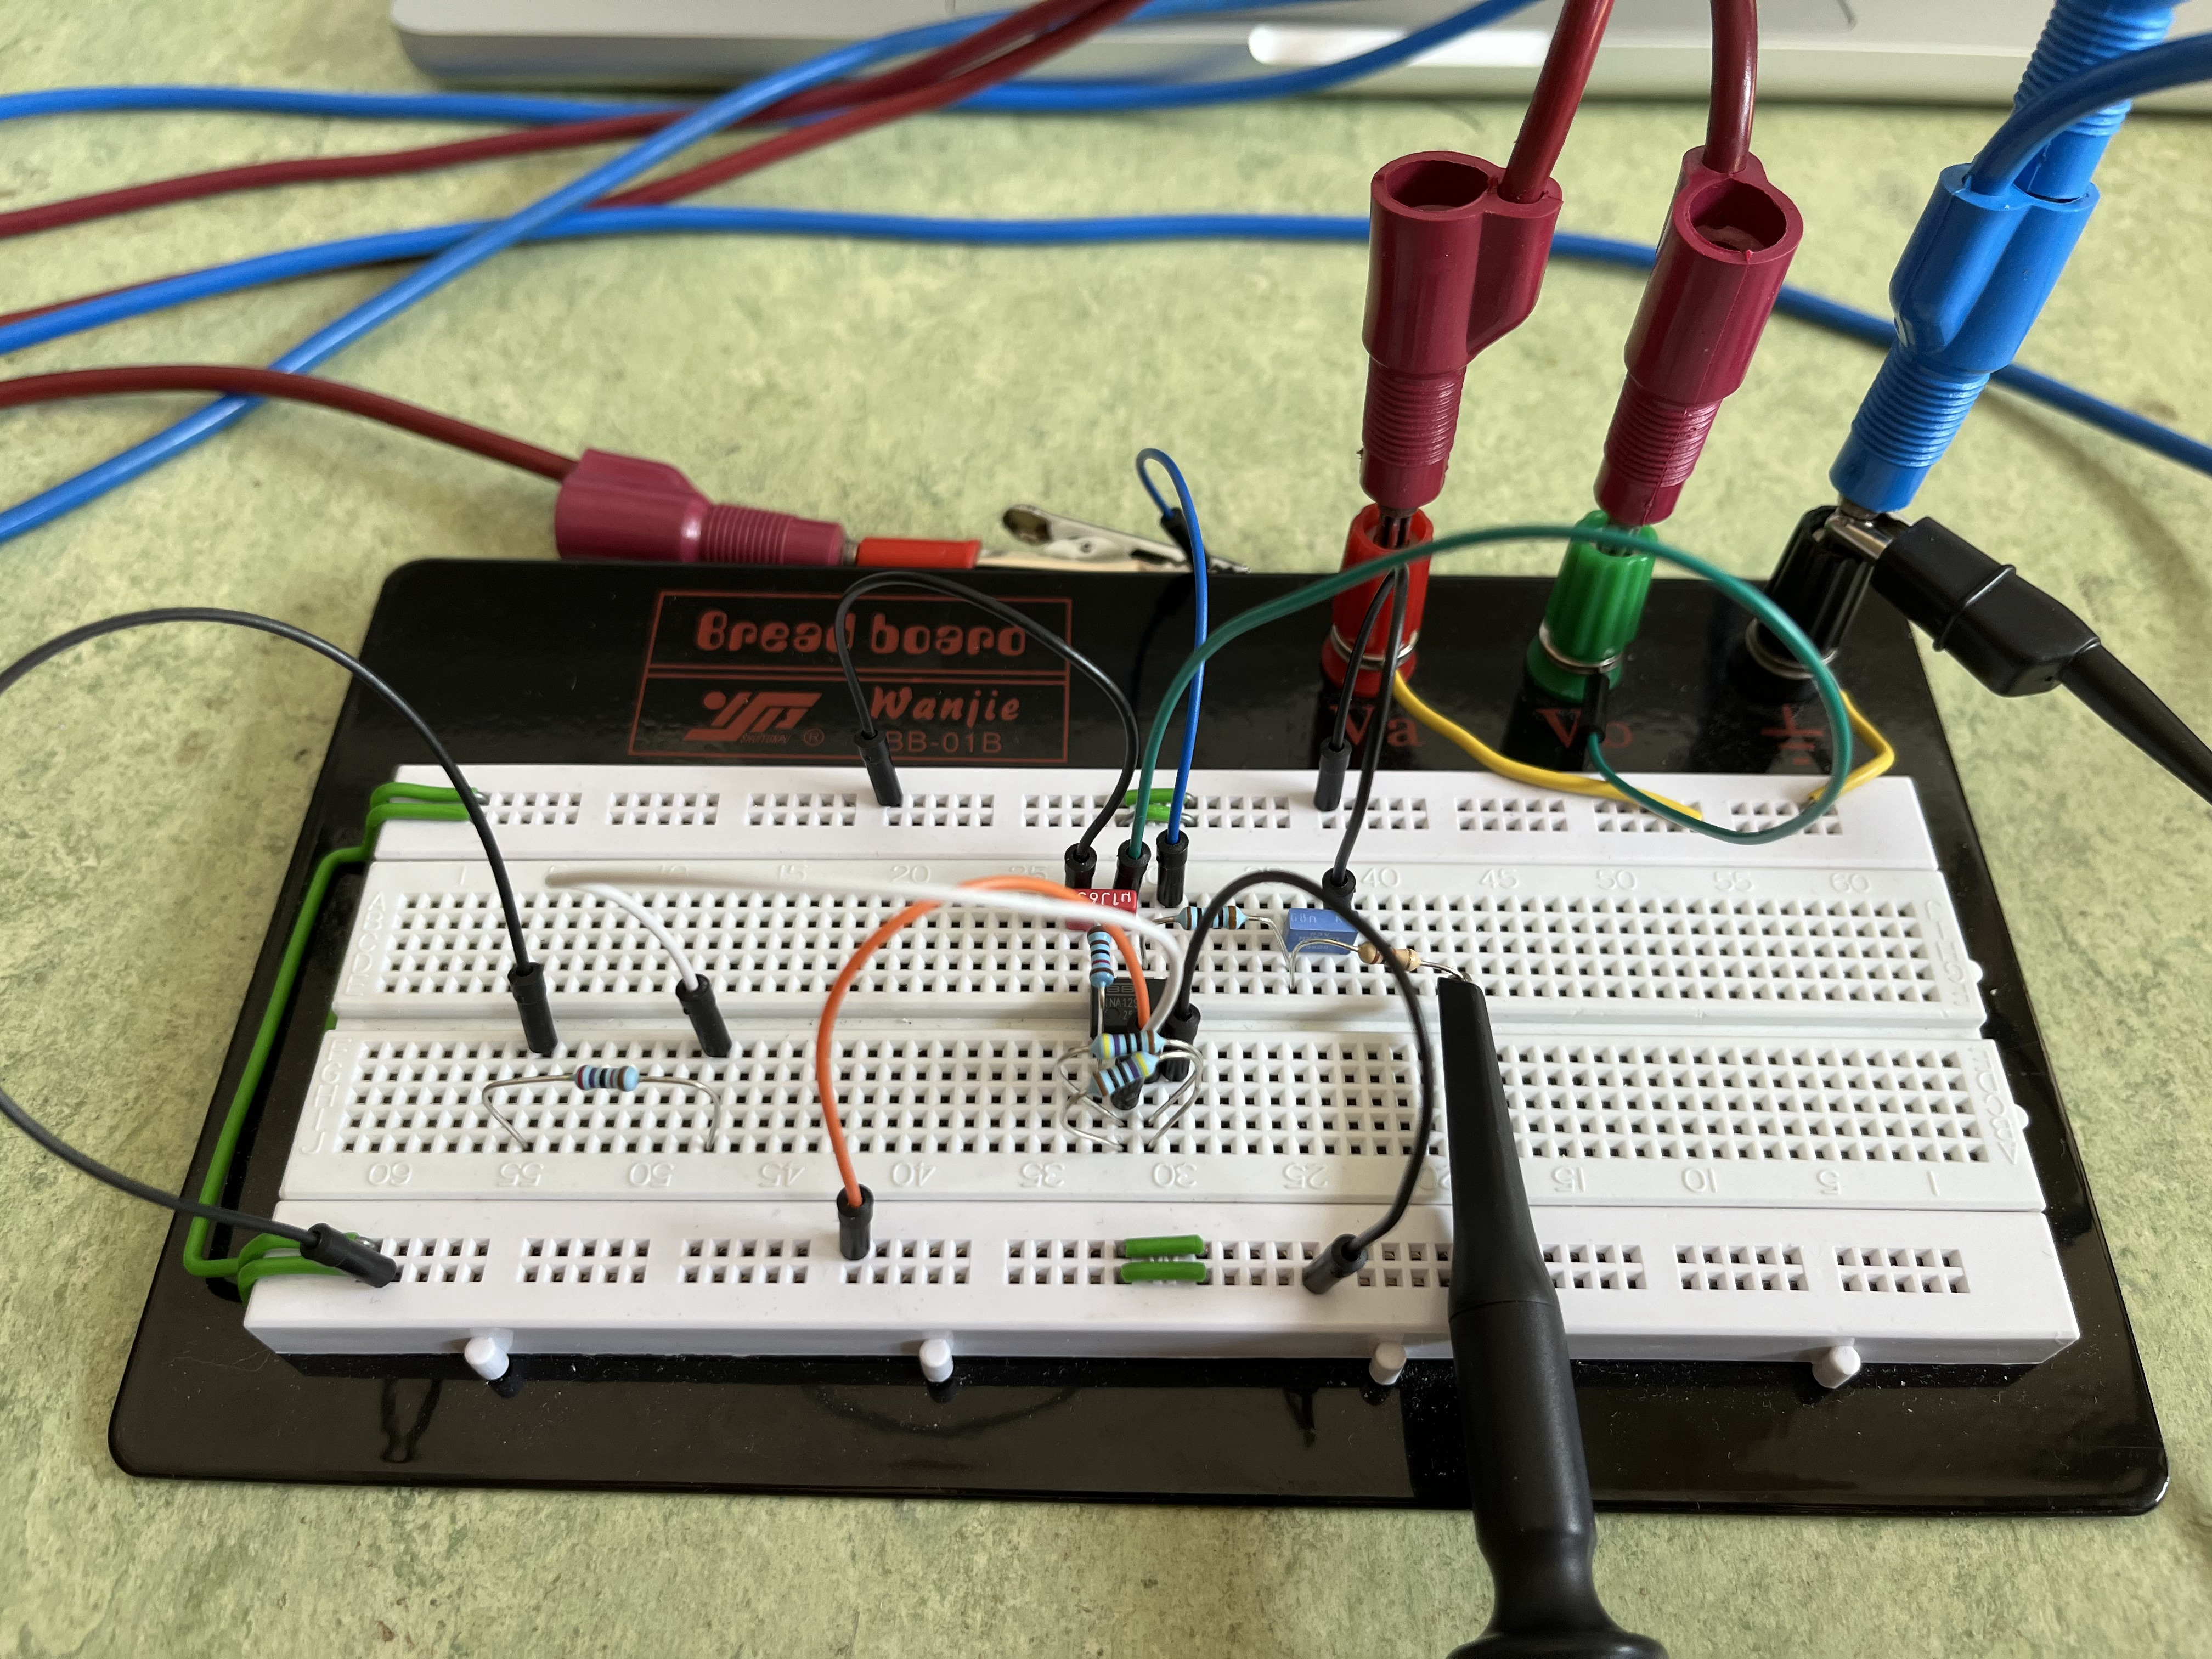
\includegraphics[width=0.8 \linewidth]{Steckbrettaufbau_Spannungsmessung_INA129}}
		%\caption*{Ladislaus Szabo}
	\end{center}
\end{figure}
\hfill \break
\hfill \break
\begin{figure}[H]
	\begin{center}
		\scalebox{1.0}
		{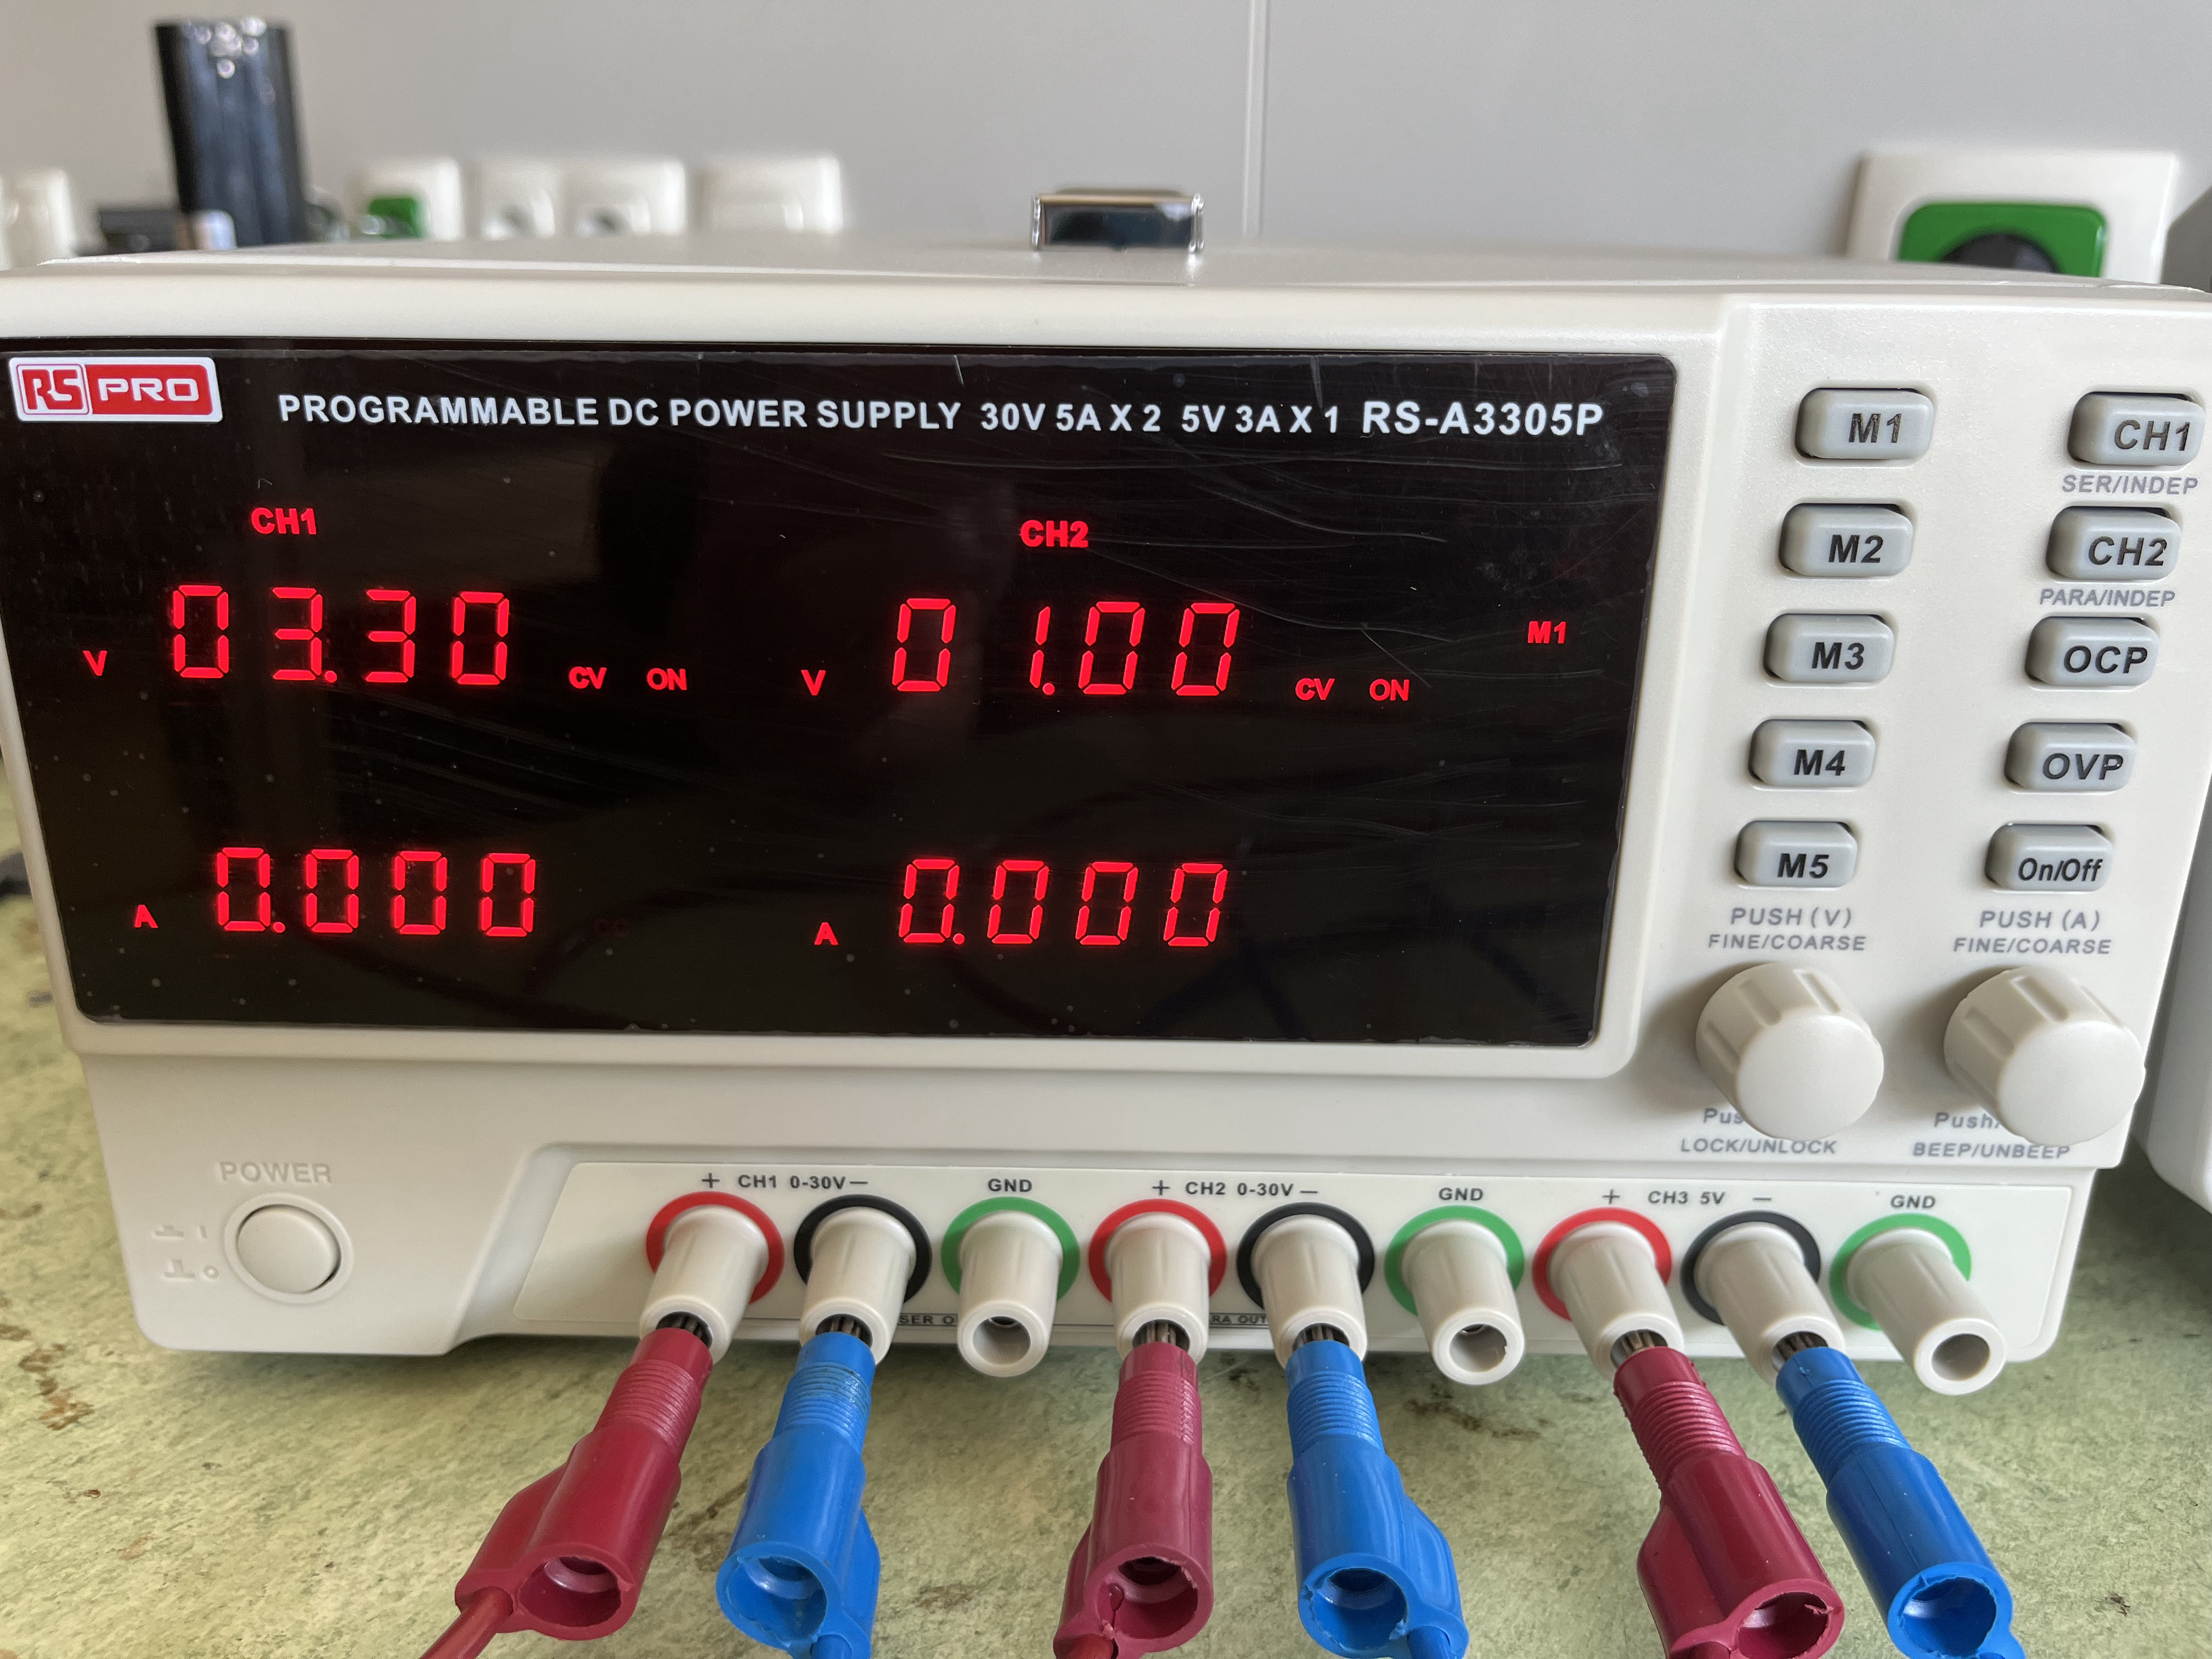
\includegraphics[width=0.8 \linewidth]{Bild_Einstellungen_Netzteil}}
		%\caption*{Ladislaus Szabo}
	\end{center}
\end{figure}
\hfill \break
+3.3V für die Versorgung des Flexsensors (Last), simuliert mit drei normalen Widerständen.\\
+1V als Referenzspannung für den INA-129.\\
+5V zur Versorgung des INA129.\\
\\

\paragraph{Messergebnisse}
\hfill \break
\hfill \break
\begin{figure}[H]
	\begin{center}
		\scalebox{1.2}
		{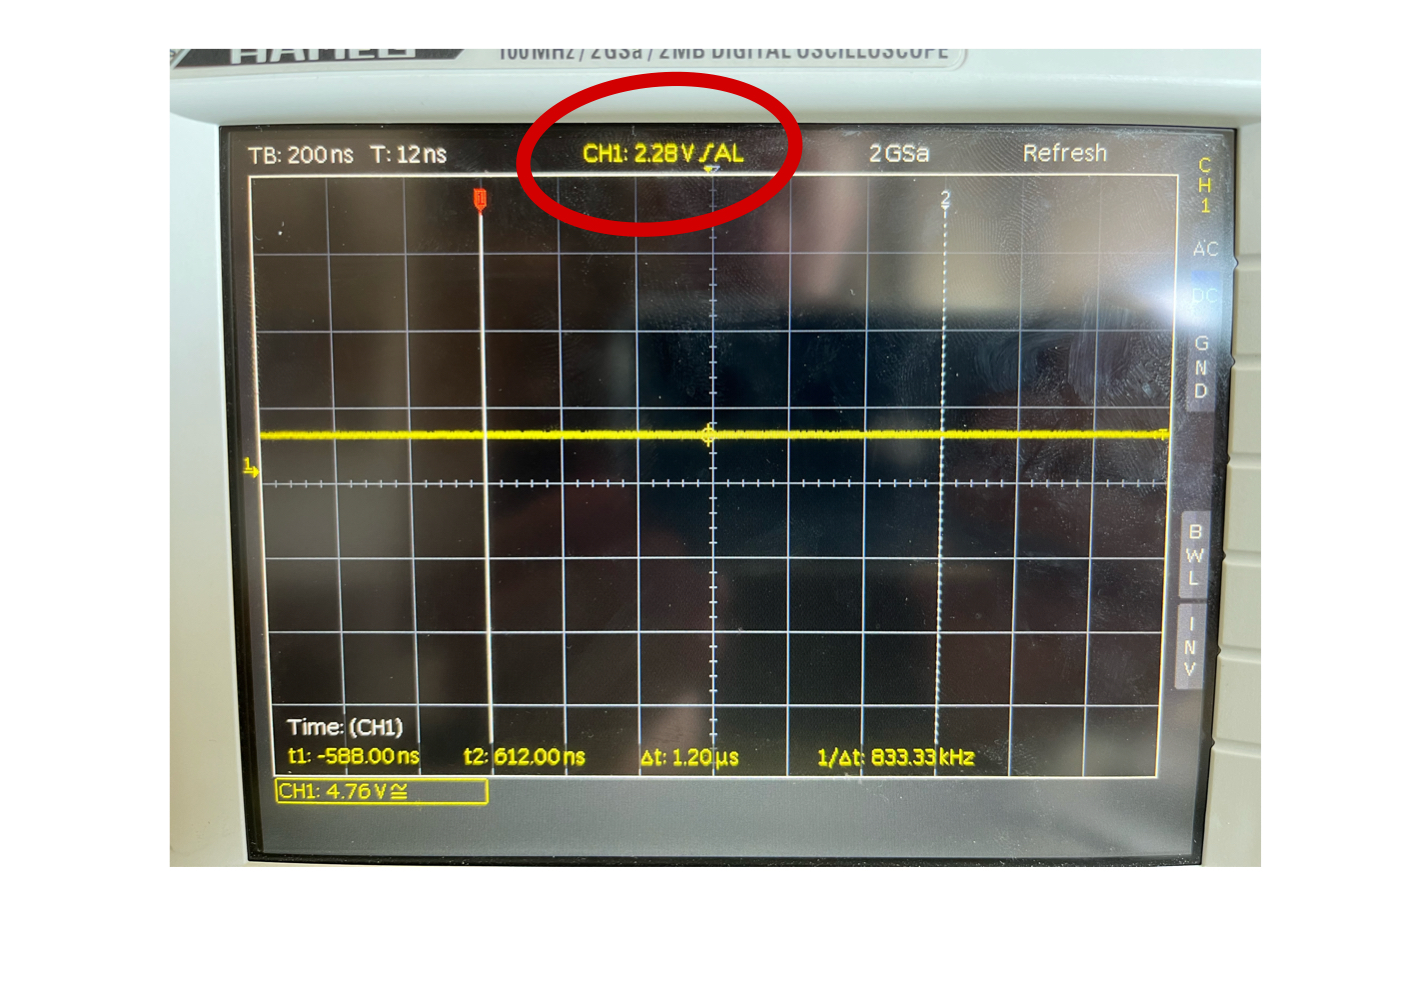
\includegraphics[width=0.8 \linewidth]{Oszibild_RL_27k}}
		%\caption*{Ladislaus Szabo}
	\end{center}
\end{figure}
Das obige Oszilloskopbild zeigt die, mit einem Tastkopf, gemessene Ausgangsspannung des Operationsverstärkers, bei einem Flexsensorwiderstand
von 27k$\Omega$. Die gemessene Spannung ist rot eingekreist und beträgt 2.28V. Da bei der Simulation in LTspice mit einem Widerstand 
von 25k$\Omega$ eine Ausgangsspannung von 2.416V resultierte, ist anzunehmen, dass 2.28V 
für den gewählten Widerstand angemessen sind. Daraus kann man schließen, dass die Schaltung
für diesen Widerstandswert des Flexsensors korrekt funktioniert.
\\
\begin{figure}[H]
	\begin{center}
		\scalebox{1.0}
		{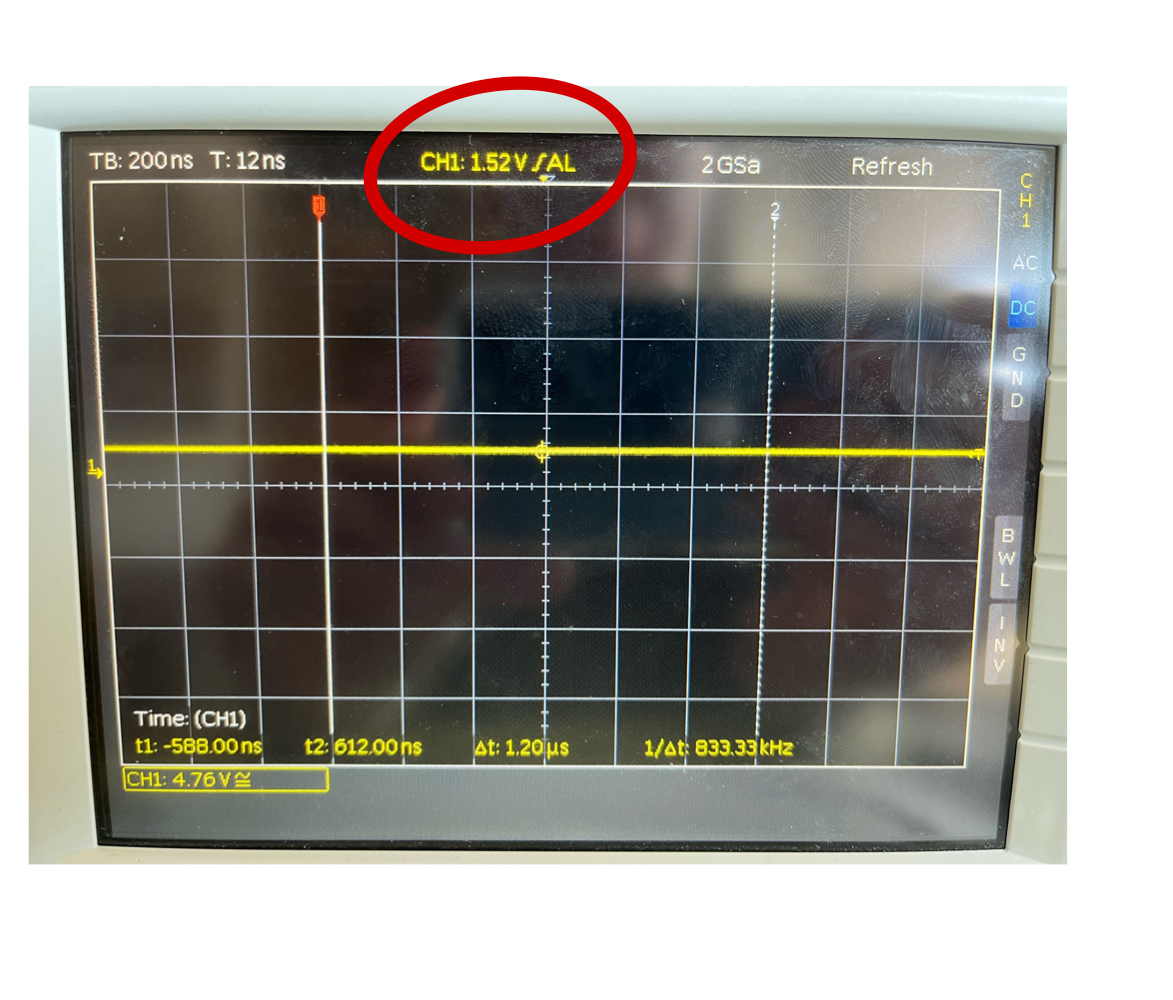
\includegraphics[width=0.8 \linewidth]{Oszibild_RL_67k}}
		%\caption*{Ladislaus Szabo}
	\end{center}
\end{figure}
\hfill \break
Nun wurde die gleiche Messung erneut durchgeführt, allerdings mit einem Flexsensorwiderstand
von 67k$\Omega$. Wir zu erwarten, ist die Ausgangsspannung des OPVs gesunken, da der 
Spannungsabfall am Shuntwiderstand nun geringer ausfällt. Zu erwarten war ein Spannungswert
von rund 1.5V. Dieser Pegel wurde mit 1.52V fast genau getroffen, wodurch die funktionsfähigkeit
der Schaltung weiter sichergestellt wurde.
\begin{figure}[H]
	\begin{center}
		\scalebox{1.0}
		{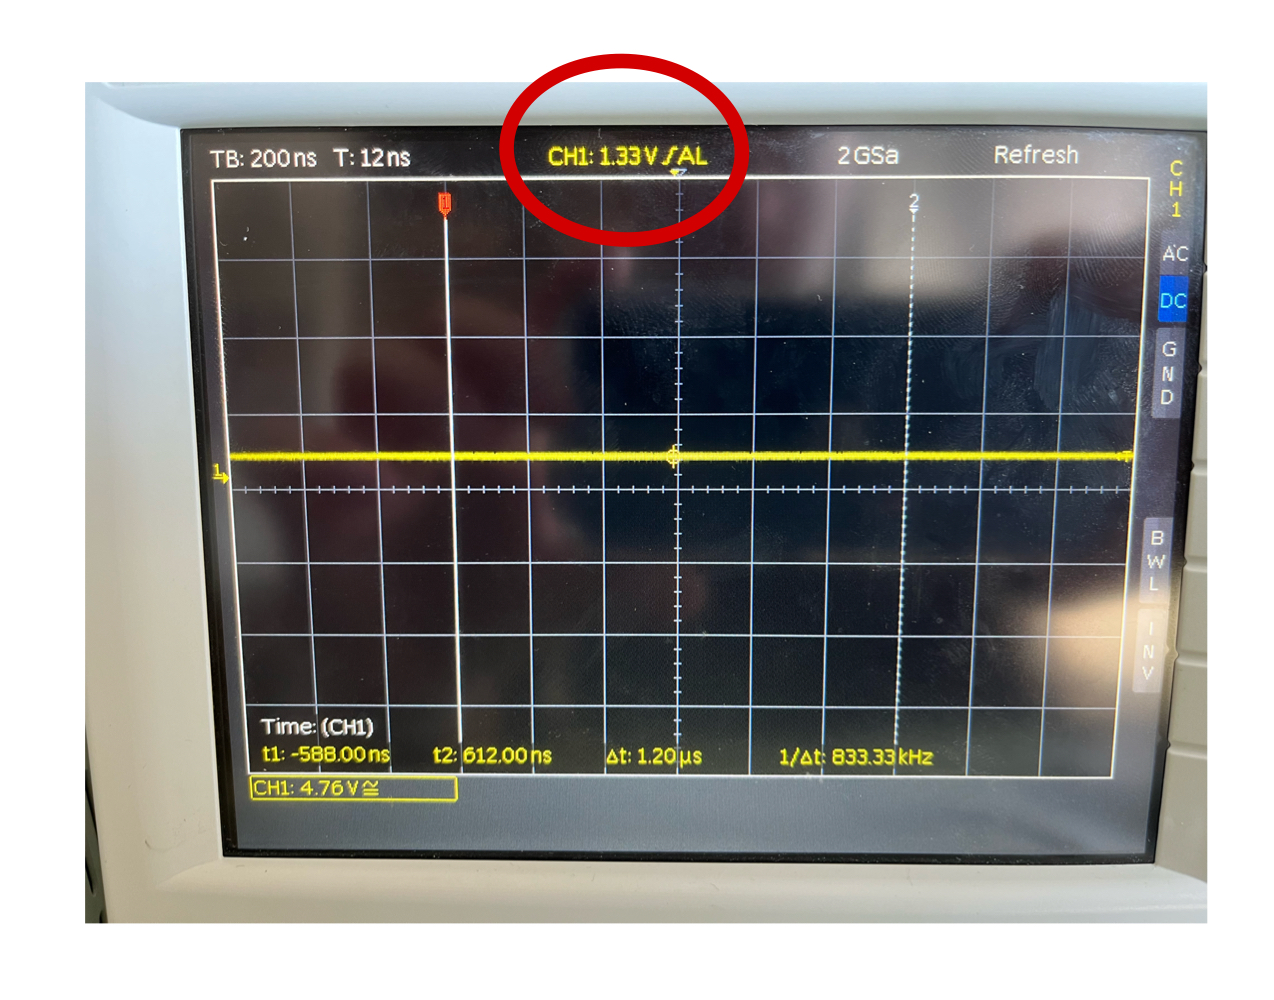
\includegraphics[width=0.8 \linewidth]{Oszibild_RL_118k}}
		%\caption*{Ladislaus Szabo}
	\end{center}
\end{figure}
\hfill \break
Schlussendlich wurde noch ein Flexsensorwiderstand von 118k$\Omega$ simuliert, um den
nahezu Maximalwert des Sensors zu simulieren. Zu erwarten waren rund 1.3V. Die Messung
bestätigt die Überlegungen, wodurch die Funktionalität dieser Schaltungskomponente bewiesen
wurde. \\
\\
Zusätzlich ist nun die Notwendigkeit einer Referenzspannung von +1V bewiesen worden, da
ohne dieser ein theoretischer Spannungspegel von nur 500mV am Ausgang des INA-129 aufgetreten
wäre.  Dies ist praktisch allerdings nicht möglich, da der OPV über keine Rail-to-Rail
Technologie verfügt, wodurch er nur eine minimale Ausgangsspannung von rund 800mV ausgeben 
kann.
\\

\subsubsection{Schaltungsdesign \textcolor{red}{Laci}}
Nach den generellen Überlegungen und Versuchsaufbauten, die zu der Entwicklung der Schaltung des Eingabesubsystems beigetragen haben, wird in diesem Punkt 
das genaue Schaltungsdesign erläutert. \\
\\
\paragraph{Externe Anschlüsse}
\hfill \break
\hfill \break
\begin{itemize}
	\item Anschluss zur Programmierung des Mikrokontrollers: \\
		  \\
		  Für die Programmierung des Mikrokontrollers wird ein USB Anschluss benötigt. Dieser sollte möglichst kompatibel mit
		  den neuesten Computern sein, weswegen wir uns für USB-C-Typ2.0 entschieden haben. Um das Serial Signal der USB Schnittstelle
		  für den Mikrokontroller lesbar zu machen, muss dieses für die UART-Kommunikation umgewandelt werden. Hierzu muss der Mikrokontroller
		  diese auch unterstützen. Mit einer Serial-UART-Bridge, wird das Signal umgewandelt. Der Chip wird von +3.3V versorgt.
		  Von der USB-Buchse werden die beiden Datenleitungen D+ und D- mit verbunden. Anschließend wird das umgewandelte Signal 
		  über die UART-Leitungen an den ESP32 Mikrokontroller übertragen. Wichtig zu beachten ist hierbei, dass die UART-Leitungen
		  ausgekreuzt sein müssen. Die Funktion der Anschlüsse RTS und DTR wird in Punkt \textcolor{red}{Mikrokontroller} erläutert. \\
		  \begin{figure}[H]
			\begin{center}
				\scalebox{0.5}
				{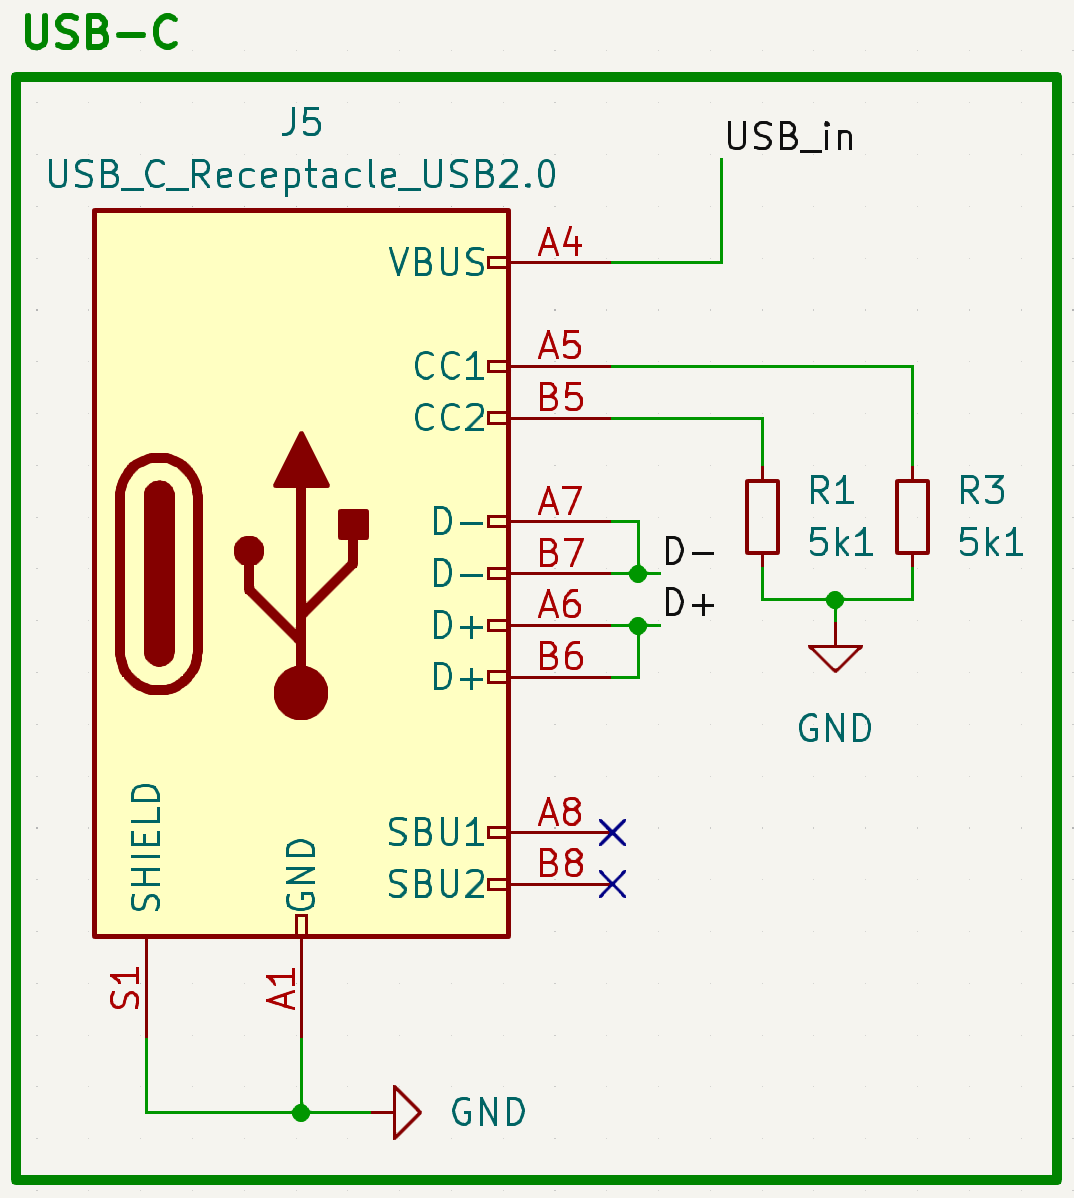
\includegraphics[width=0.8 \linewidth]{USB_C_Schaltplan_Handschuh}}
				%\caption*{Ladislaus Szabo}
			\end{center}
		\end{figure}
	\item Anschluss der Flexsensoren: \\
		  \\
		  Die Flexsensoren könnten natürlich einfach angelötet werden, jedoch ist die einfache Wartung bei einem fehlerhaften
		  Sensor ebenfalls zu berücksichtigen. Aufgrund dessen wird eine 6-Pin-JST-Buchse als Anschluss verwendet. Alle GND-Pins
		  werden auf einen zusammengefasst, um möglichst viel Platz zu Sparen. \\
		  \begin{figure}[H]
			\begin{center}
				\scalebox{0.5}
				{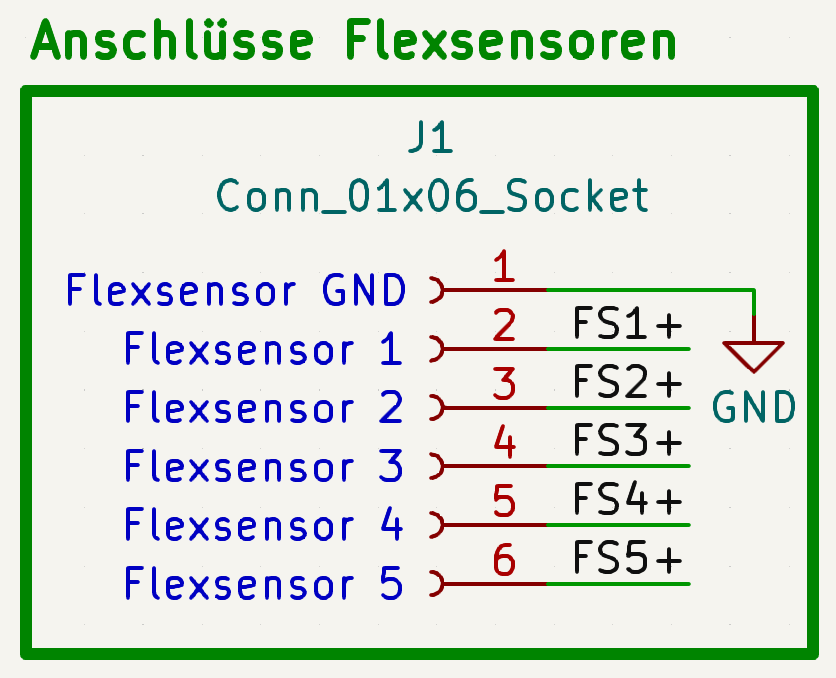
\includegraphics[width=0.8 \linewidth]{JST_Flexsensoren_Schaltplan_Handschuh}}
				%\caption*{Ladislaus Szabo}
			\end{center}
		\end{figure}
	\item Anschluss des Akkus: \\
		  \\
		  Der Akku wird ebenfalls mit einer JST-Buchse mit der Schaltung verbunden anstatt diesen anzulöten. Da der Akku einen
		  Versorgungs -und GND-Anschluss hat, wird eine 2-Pin-JST-Buchse verwendet. \\
		  \begin{figure}[H]
			\begin{center}
				\scalebox{0.5}
				{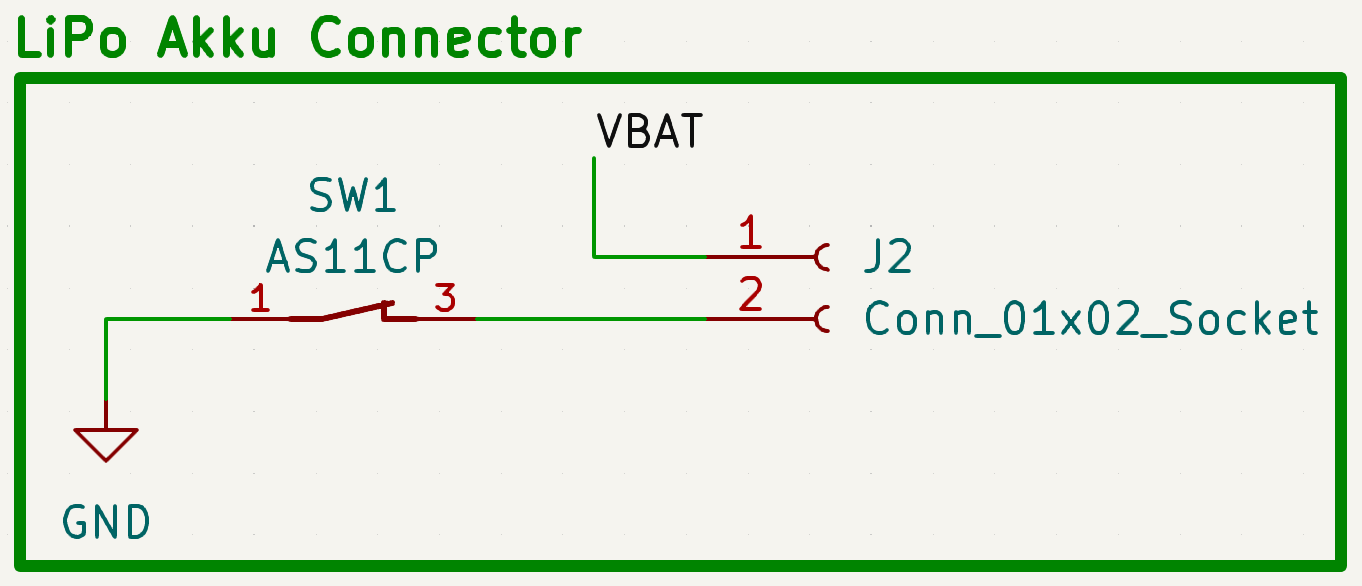
\includegraphics[width=0.8 \linewidth]{JST_Akku_Schaltplan_Handschuh}}
				%\caption*{Ladislaus Szabo}
			\end{center}
		\end{figure}\end{itemize}

\paragraph{Mikrokontroller} 
\hfill \break
\hfill \break
Der ESP32-Chip wird mit +3.3V versorgt. Wichtig zu beachten ist dadurch, das ein Logic-HIGH somit auch 3.3V und nicht 5V ist!
Die Versorgung wird mit einem Kondensator stabilisiert. Für alle Busleitungen, also I2C und UART, wurden Widerstände in Serie
hinzugefügt, um die Kommunikationsleitungen vor Spannungsspitzen oder Überspannung zu schützen. Die Funktion wäre auch ohne diese
gegeben. Für die Datenleitungen SDA und SCL des I2c Busses sind zwei $10k\Omega$ PullUp-Widerstände vorgesehen. Zusätzlich 
wird ebenfalls der Anschluss IO16 mit einem PullUp-Widerstand auf 3.3V gezogen, da dies so vom Datenblatt vorgegeben wird. 
Die Funktionen der einzelnen Anschlüsse werden in den folgenden Punkten gemeinsam mit den damit verbundenen Bauteilen näher erläutert. \\
\begin{figure}[H]
	\begin{center}
		\scalebox{0.5}
		{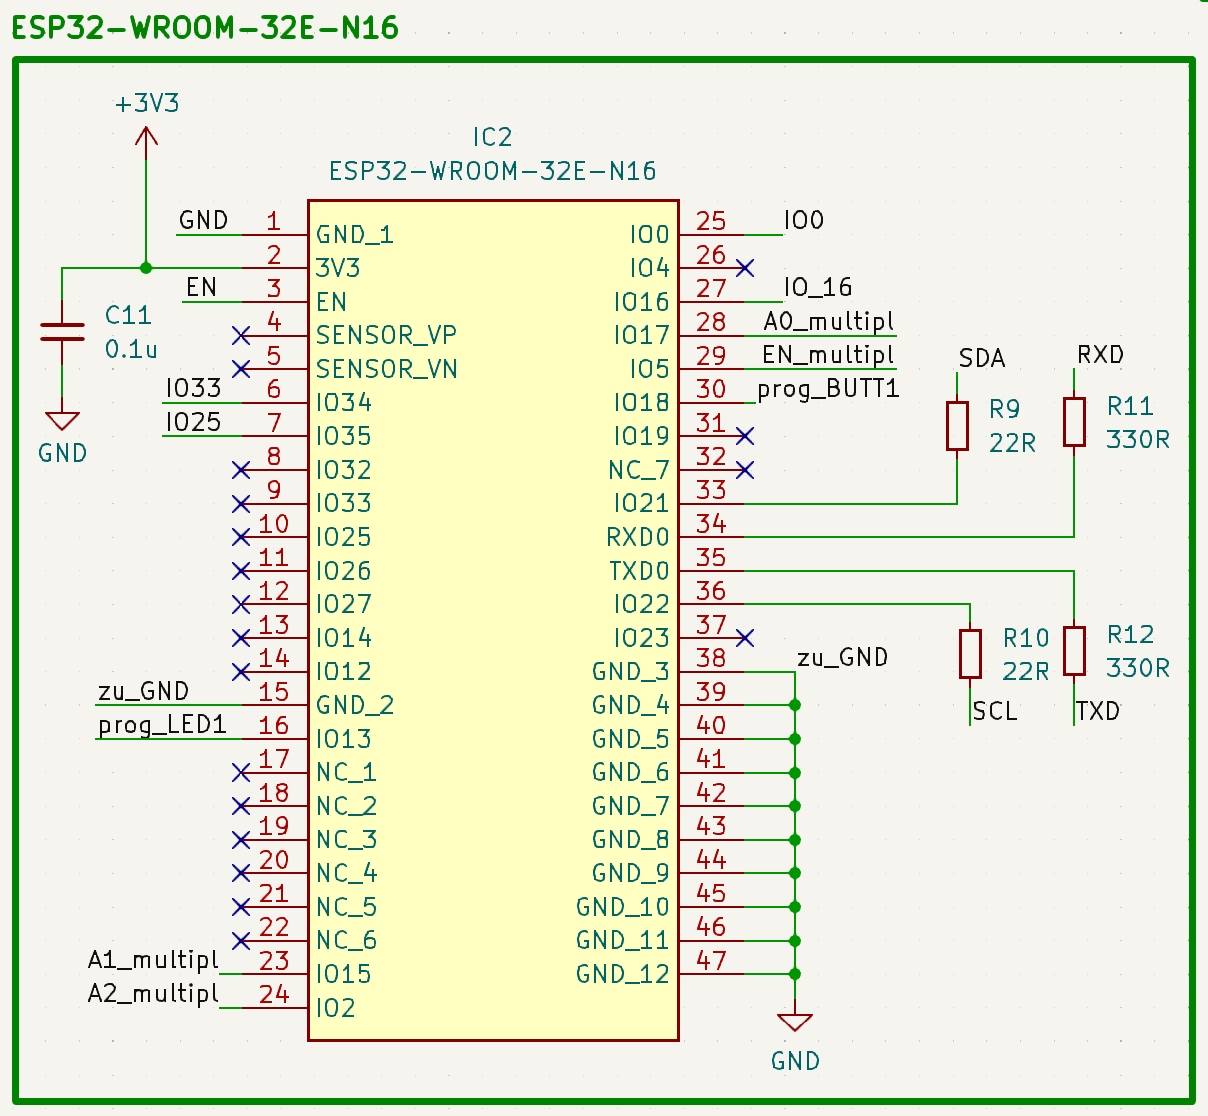
\includegraphics[width=0.8 \linewidth]{ESP32_Schaltplan_Handschuh}}
		%\caption*{Ladislaus Szabo}
	\end{center}
\end{figure}

\paragraph{Mikrokontroller Buttons}
\hfill \break
\hfill \break
In der Schaltung sind drei Taster verbaut. Diese sind alle mit dem Mikrokontroller verbunden und erfüllen verschiedene Funktionen.
\begin{itemize}
	\item Upload Button: \\
		  \\ 
		  Dieser Button ist mit dem IO0 Anschluss des ESP32 verbunden und muss bei dem Hochladen von Code kurzzeitig gedrückt 
		  werden, um den Mikrokontroller in den Upload-Modus zu versetzen. Der Pin IO0 ist standardmäßig für diese Funktion vorgesehen
		  und sollte für nichts anderes verwendet werden. 
	\item Reset Button: \\
		  \\
		  Dieser Button ist mit dem EN (Enable) Anschluss des ESP32 verbunden. Die Funktion dieses Tasters ist es, den ESP32 jederzeit 
		  zurücksetzen zu können falls dieser abstürtzt oder ein anderweitiges Problem auftritt, durch das dieser nicht mehr korrekt
		  funktioniert.
	\item Progrmmable Button: \\
		  \\
		  Die Funktion dieses Buttons kann frei durch den programmierten Code gewählt werden. 
\end{itemize}

\paragraph{Status LEDs}
\hfill \break
\hfill \break
Die beiden Leuchtdioden sind als Statusanzeige gedacht. Eine POWER LED, die immer leuchtet wenn die Schaltung mit +5V
versorgt wird. Die Funktion der anderen LED ist, sowie bei einem Button, frei wählbar und ist deswegen mit Pin IO13 des ESP32
verbunden. \\
\begin{figure}[H]
	\begin{center}
		\scalebox{0.5}
		{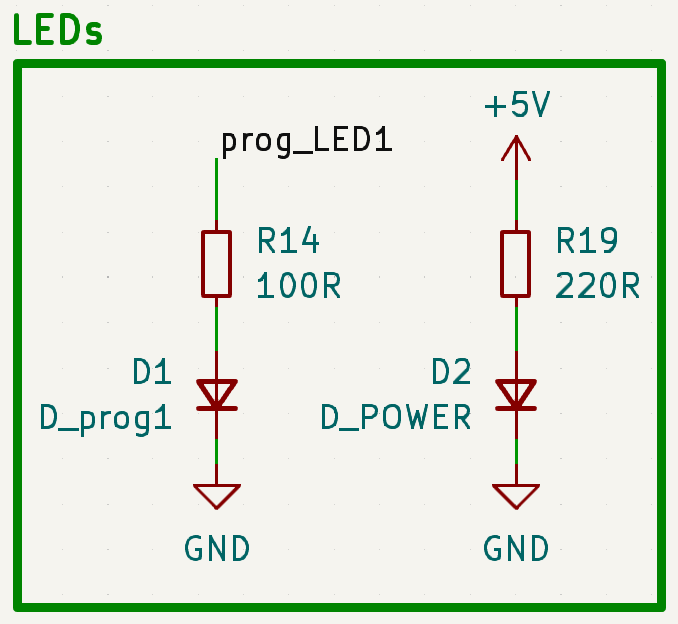
\includegraphics[width=0.8 \linewidth]{LEDs_Schaltplan_Handschuh}}
		%\caption*{Ladislaus Szabo}
	\end{center}
\end{figure}

\paragraph{Multiplexer}
\hfill \break
\hfill \break
Der Multiplexer schaltet zwischen allen Flexsensoren durch und vermeidet somit die Messschaltung fünf mal bauen zu müssen. 
Die Verbindung zum ESP32 erfolgt über drei digitale Addresspins und einen Enable Pin. Je nachdem welche Bitkombination übermittelt
wird, ändert sich die interne Schalterposition und somit der gerade aktive Kanal zur Messung eines Flexsensors. \\
\\
\paragraph{Operationsverstärker}
\hfill \break
\hfill \break
Für das Auslesen der Flexsensoren, wird eine Schaltung, wie in Punkt "Auslesen der Sensoren" beschrieben, benötigt. Da am
Shuntwiderstand nur sehr wenig Spannungsabfall auftritt und daher die Spannungsdifferenz zwischen positivem und negativem 
Verstärkereingang sehr klein ist, muss das Signal verstärkt werden. Hierfür wird der INA129 Instrumentenverstärker verwendet.
Dieser wird mit 5V versorgt, was für einen OPV eine relativ geringe Versorgungsspannung ist. Da die maximale Eingangsspannung
der Verstärkereingänge allerdings nie mehr als 3.3V beträgt, ist dies kein Problem. \\
\\
Die +1V Spannungsreferenz ist notwendig, da der ausgewählte Operationsverstärker nicht über Rail-to-Rail Technologie besitzt. 
Die kleinstmögliche Spannungsdifferenz am Eingang des OPV, wenn der Flexsensor seinen maximalen Widerstand von
$125k\Omega$ erreicht, beträgt nur 6.3mV. Aufgrund der fehlenden Rail-to-Rail Fähigkeit, muss die Ausgangsspannung des OPV deshalb
auf mindestens 800mV angehoben werden, um eine korrekte Funktion des OPVs zu gewährleisten. Deshalb wird eine Referenzspannung
von 1V verwendet. \\
\begin{figure}[H]
	\begin{center}
		\scalebox{0.5}
		{\includegraphics[width=0.8 \linewidth]{Operationsverstärker_Schaltplan_Handschuh}}
		%\caption*{Ladislaus Szabo}
	\end{center}
\end{figure}

\paragraph{Analog-Digital-Wandler}
\hfill \break
\hfill \break
Der Analog-Digital-Wandler ist dafür zuständig, die analogen Werte, vom Ausgang des Operationsverstärkers kommend, in digitale 
Signale umzuwandeln. Der OPV und der ADC sind über das Label toADC verbunden. Da der Chip über 3.3V versorgt wird, befindet
sich der mögliche Aussteuerbereich zwischen 0V und 3.3V. Wie im Punkt Umwandlung der Diferenzwerte in ein geeignetes Format berechnet, 
hat der ADC in unserer Schaltung ein LSB von 3.22mV. Da wir wissen, dass die kleinste Spannungsdifferenz am Shuntwiderstand 6.3mV
ist und diese auch noch mit dem Faktor 46 verstärkt wird, kann festgestellt werden, dass der ADC mehr als genau genug für unsere
Anwendung ist. Dies ist ein Vorteil, da bei der Programmierung anschließend nicht zwischen einzelnen ADC-Stufen unterschieden werden
muss, sondern immer mehrere LSBs Unterschied auftritt. Die aktualisierten Werte, werden über die beiden I2C Leitungen an den 
Mikrokontroller übertragen. \\
\\
\begin{figure}[H]
	\begin{center}
		\scalebox{0.5}
		{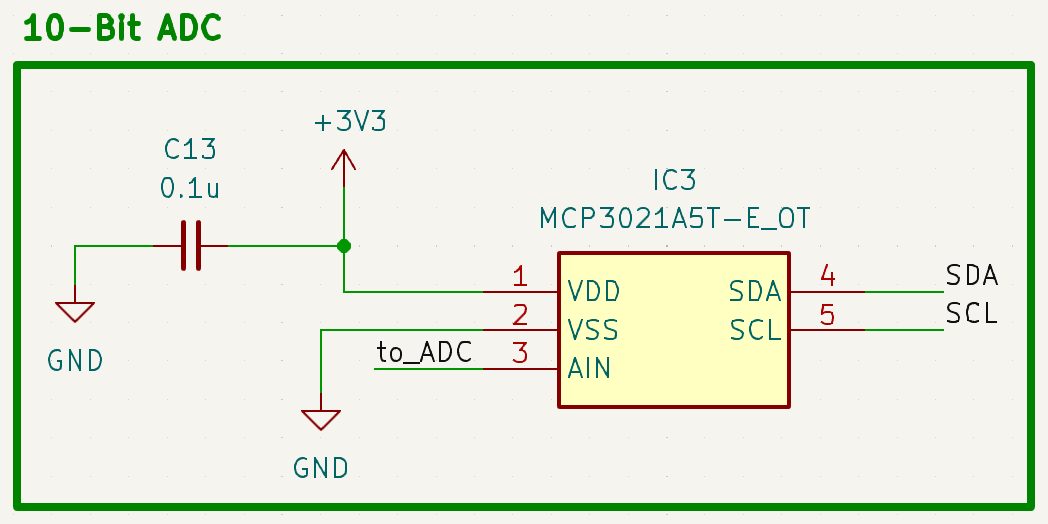
\includegraphics[width=0.8 \linewidth]{ADC_Schaltplan_Handschuh}}
		%\caption*{Ladislaus Szabo}
	\end{center}
\end{figure}

\paragraph{Gyroskop-Sensor}
\hfill \break
\hfill \break
Der Gyroskopsensor ist dafür zuständig die Drehung des Handschuhs in X, Y -und Z Richtung warzunehmen. Die Versorgung basiert 
auf 3.3V und die Datenübertragung erneut mittels I2C-Bussystem. Der Unterschied bei diesem Chip ist allerdings, dass mehrere ADCs
integriert sind, um die Positionsdaten der Achsen schon digitalisiert an den Mikrokontroller zu übergeben. AD0 wird dabei verwendet
um die Adresse des Mikrochips festzulegen. Diese wird später benötigt um mit dem Sensor Daten austauschen zu können.
\\
\begin{figure}[H]
	\begin{center}
		\scalebox{0.5}
		{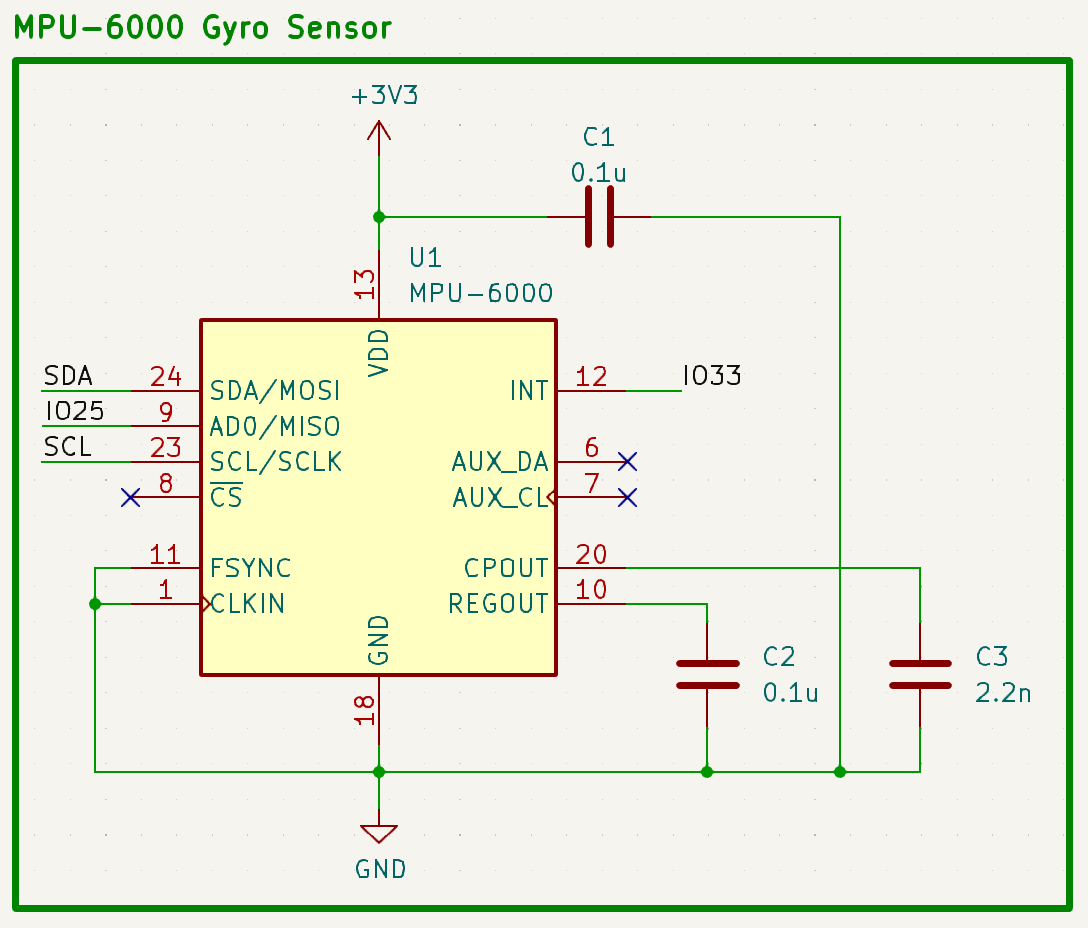
\includegraphics[width=0.8 \linewidth]{Gyro_Schaltplan_Handschuh}}
		%\caption*{Ladislaus Szabo}
	\end{center}
\end{figure}
\hfill \break
Am Pin CLKIN hätte man die Möglichkeit einen externen Referenztaktgeber anzuschließen. Bei unserer Anwendung ist der integrierte 
Taktgeber allerdings völlig ausreichend, weswegen der Anschluss mit GND verbunden und damit deaktiviert wurde. Der CS Pin wird nur
für die SPI Kommunikation benötigt, weshalb dieser ebenfalls deaktiviert wurde. Das gleiche gilt für den Anschluss FSYNC. Die beiden
AUX-Anschlüsse könnte man verwenden, um mit anderen I2C fähigen Sensoren direkt zu kommunizieren. Da dies allerdings unser einziger
Sensorchip mit dieser Fähigkeit ist, bleiben die beiden Pins auch nicht verbunden. Die Kondensatoren sind vom Hersteller im Datenblatt
vorgesehen und gewährleisten einen stabilen Betrieb. \\
\\
\paragraph{Akku Versorgung}
\hfill \break
\hfill \break
\begin{figure}[H]
	\begin{center}
		\scalebox{0.5}
		{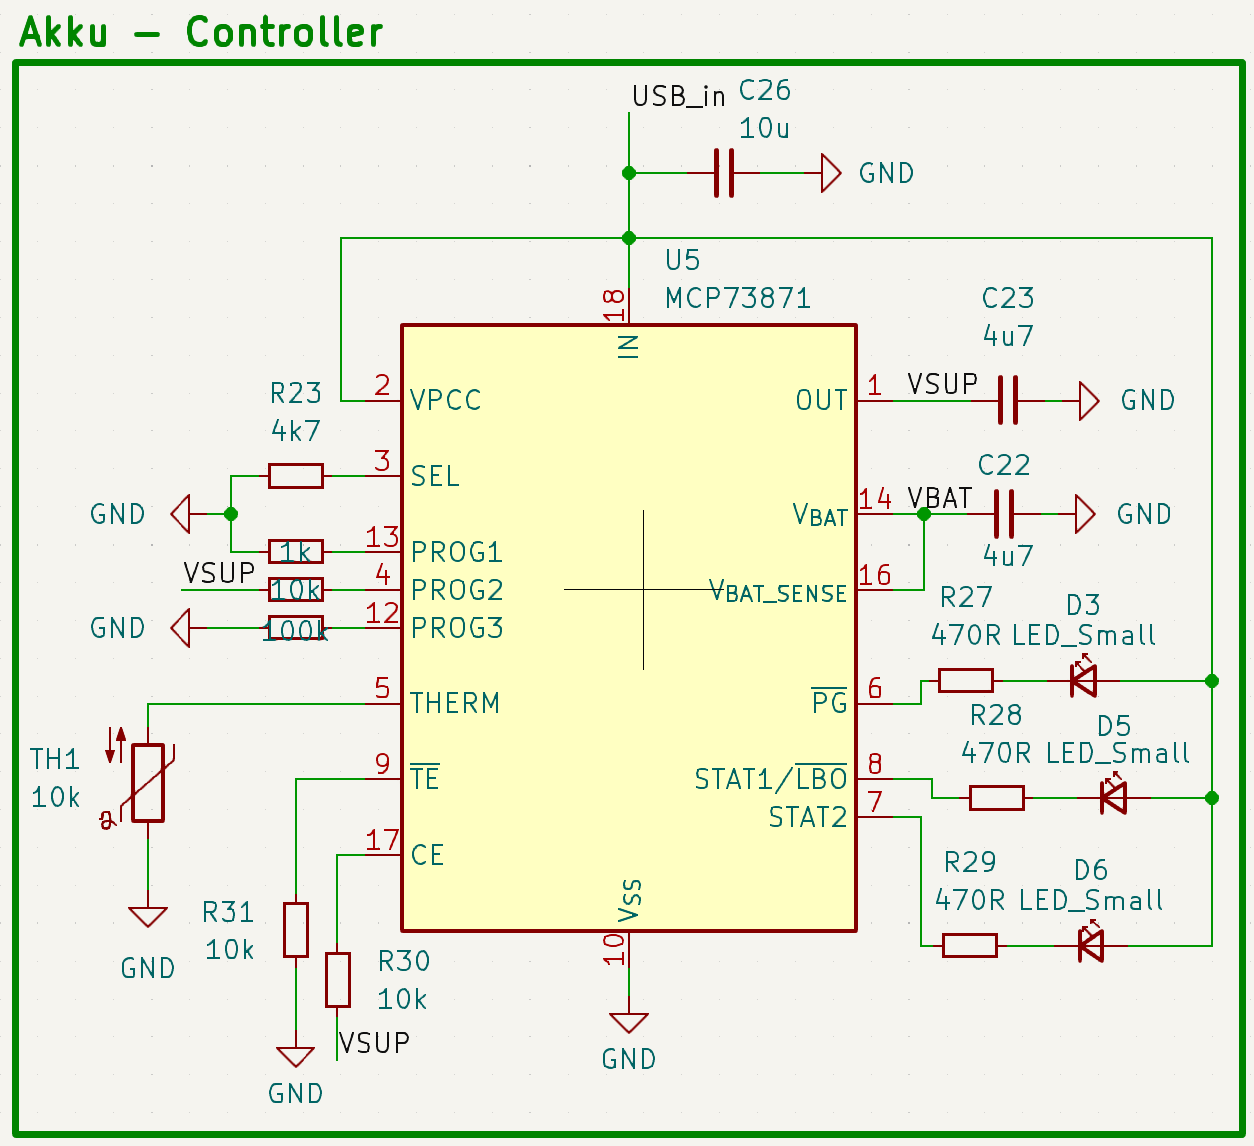
\includegraphics[width=0.8 \linewidth]{Akku_Controller_Schaltplan_Handschuh}}
		%\caption*{Ladislaus Szabo}
	\end{center}
\end{figure}

\begin{figure}[H]
	\begin{center}
		\scalebox{0.5}
		{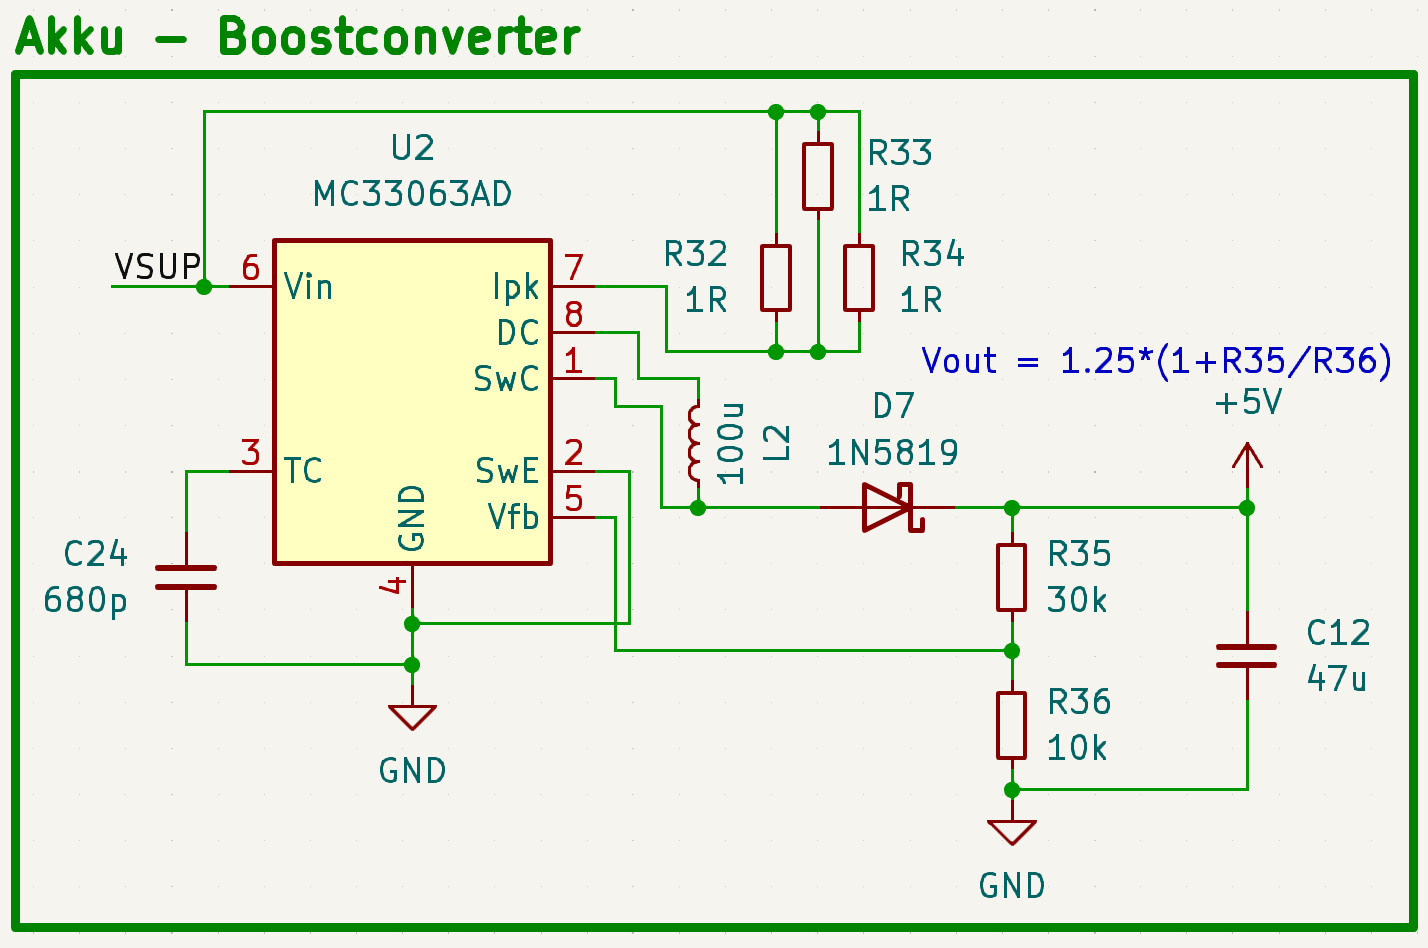
\includegraphics[width=0.8 \linewidth]{Akku_Boostconverter_Schaltplan_Handschuh}}
		%\caption*{Ladislaus Szabo}
	\end{center}
\end{figure}

\begin{figure}[H]
	\begin{center}
		\scalebox{0.5}
		{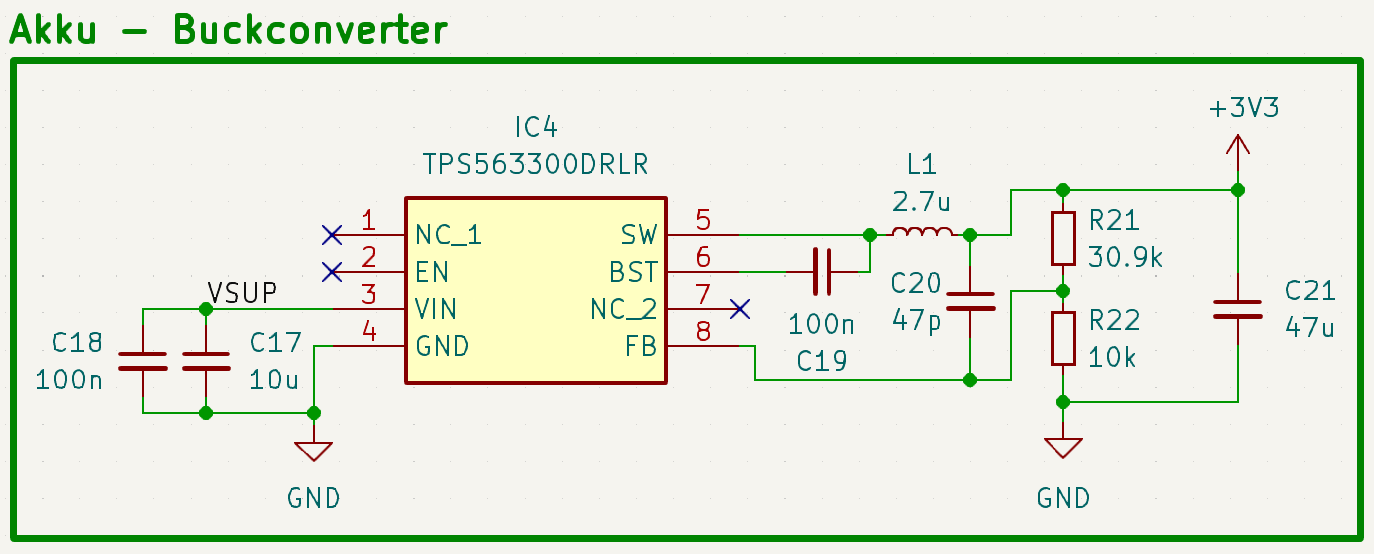
\includegraphics[width=0.8 \linewidth]{Akku_Buckconverter_Schaltplan_Handschuh}}
		%\caption*{Ladislaus Szabo}
	\end{center}
\end{figure}

\subsubsection{Platinendesign \textcolor{red}{Laci}}

\subsection{Roboterhand}

\subsubsection{Grundlegende Vorraussetzungen}
Die Roboterhand ist die Ausgabe des Gesamtsystems und wird vom Eingabesubsystem gesteuert. Jeder Finger wird von einem Motor 
bewegt. Die ankommenden Daten müssen interpretiert und anschließend in ein geeignetes Format zur Ansteuerung der Motoren
umgewandelt werden. Zusätzlich zu dieser grundlegenden Funktionalität der Ansteuerung, müssen auch noch einige weitere Aspekte
beachtet werden. Hier sind zum Beispiel die möglichst geringe Größe der Schaltung und die trotzdem ausgiebigen Funktionen 
zu nennen. Dazu zählen visuelle Indikatoren für diverse Parameter, Schalter und Taster, Anschlüsse und Erweiterungsmöglichkeiten.
Die detailierten Entwicklungs -und Designschritte, werden in den folgenden Punkten näher erläutert. \\

\subsubsection{Überlegungen, Simulationen und Berechnungen \textcolor{red}{Laci}}
\paragraph{Aktorik zur Fingerbewegung}
\hfill \break
\hfill \break
Bei der Aktorik zur Bewegung der Roboterfinger, gibt es, wie bei Sensorik zur Erfassung der Bewegungen, ebenfalls unzählige Methoden
und Konzepte zur Auswahl. Bei schon etablierten Herstellern von bionischen Händen werden fast ausschließlich lineare DC Motoren 
verwendet. Diese sind sehr hochpräzise, sehr gut gefertigt und haben für ihre Größe sehr viel Kraft. Nachteile sind allerdings
die hohen Preiseund die vergleichweise kompliziertere Ansteuerung. Außerdem sollten diese Motoren in präzise gefertigten Produkten
Anwendung finden, die möglichst wenig Reibung aufweisen und gelagerte Gelenke haben. Da wir in der Schule die Möglichkeit zur Fertigung 
eines solchen Produkts nicht haben und dies ebenfalls zu teuer wäre, haben wir uns entschieden diese Art der Aktorik, obwohl es die beste Wahl wäre,
nicht zu verwenden. Stattdessen haben wir uns für die Verwendung von Servo Motoren entschieden, die wesentlich billiger und einfacher anzusteuern sind und trotzdem mehr als
genügend Kraft haben. Der Nachteil bei diesen Motoren ist allerdings die Größe, wodurch unser Endprodukt ziemlich sicher etwas größer als gehofft
ausfallen wird. \\

\paragraph{Datenempfang}
\hfill \break
\hfill \break
Um den Datentransfer möglichst einfach zu gestallten und keine Kompatibilitätsprobleme zu haben, entschieden wir uns den gleichen Mikrokontroller
wie beim Eingabesubsystem zu verwenden. Dies ermöglicht eine relativ einfache Datenübertragung ohne zusätzliche Antennen. Werden Daten empfangen,
so wird die Software am Chip aktiv, die in Punkt (\textcolor{red}{Verweis auf Roboterhand Softwarebeschreibung}) näher beschrieben wird. Der
Entschluss zur Verwendung dieser \"identischen\" Systeme, wurde relativ rasch getroffen, da wir genug andere Schwierigkeiten haben werden und 
die Funkübertragung nicht dazu zählen soll. Genauere Designanforderungen, zum Layout der integrierten Antenne, werden in Punkt 7.2.5 erklärt.

\paragraph{Ansteuerung der Motoren}
\hfill \break
\hfill \break
Nachdem die Daten in Software verarbeitet wurden, müssen nun die Servomotoren angesteuert werden. Da diese über ein PWM-Signal (\textcolor{red}{siehe Punkt 4.3})
angesteuert werden, stellt sich die Frage ob man dies direkt über den Mikrokontroller realisiert, oder mithilfe einer PWM-Controller-Schaltung.
Da wir eine Mindestanzahl von fünf Servomotoren haben und auch für zukünftige Erweiterungen bereit sein möchten, haben wir uns für die Ansteuerung
via Servo-Controller entschieden. \\
\\
Bei der Ansteuerung der Motoren ohne Controller, ist das Problemm, dass für jeden Servomotor ein eigener Pin des Mikrokontrollers benötigt wird.
Dies ist nicht gerade Vorteilhaft, weil dadurch zwangsweise andere Funktionen des Mikrokontrollers, die nur mit bestimmten Pins funktionsfähig sind,
außer Kraft gesetzt werden. 


\paragraph{Positionsmessung der Fingerstellung}
\hfill \break
\hfill \break

\subsubsection{Versuchsaufbauten und Messungen \textcolor{red}{Laci}}
\subsubsection{Schaltplandesign \textcolor{red}{Laci}}
\subsubsection{Platinendesign \textcolor{red}{Laci}}

%--------------------------------------------------------------------------
%--------------------------------------------------------------------------

\section{Software Realisierung}

\subsection{Handschuh}
\subsubsection{Konzepte und Überlegungen \textcolor{red}{Fabian}}
\paragraph{Datenübertragung}
\hfill \break
\hfill \break
Es gibt viele Möglichkeiten die Werte, die man von jedem einzelnen Flexsensor ausliest, zu übertragen. Wichtig ist es, dass 
dies einfach und auf eine sehr stabile Weise funktioniert. Werden nämlich Daten fehlerhaft oder nur teilweise übertragen, dann 
wirkt sich das auf der Empfängerseite drastisch aus. Es könnten dadurch unerwartete Fehler passieren beziehungsweise könnte die 
Roboterhand von einem unstabilen System sehr hohe Schwankungen der Werte andauern wahrnehmen, was zu einer durchgängigen 
Belastung der Servos führen würde. Das ist zwar nicht allzu schlimm, aber verbraucht unnötig Ressourcen. Anfangs war Bluetooth 
die favorisierte Option, da man im Alltag immer wieder mit Geräten zu tun hat, die Bluetooth als Standard der Funkübertragung 
verwenden. Allerdings haben wir uns später dann aber für Wifi entschieden, da angenommen wurde, dass wir große Mengen an Daten 
versenden. Dies ist nun aber nicht nötig, da nur die Widerstandswerte, die über einen ADC umgerechnet werden, nun versendet 
werden Deshalb haben wir nach einer neuen Möglichkeit gesucht, die einfacher zu realisieren ist. Schlussendlich wurde es dann 
ESP-NOW, das auf 2,4GHz funkt und am ehesten mit Wifi verglichen werden kann. Es können pro Sendung 250 Byte gesendet werden. 
Ebenso ist eine Kommunikation zwischen mehreren ESP32 in beide Richtungen möglich. Der Standard gilt allerdings wirklich nur 
für den ESP32, was allerdings aufgrund der Wahl von nur diesem letztgenannten, keine Probleme darstellt. ESP-NOW sendet auf dem 
802.11 Protokoll, wie auch Wifi es macht. Der Vorteil liegt aber klar in der Energieeffizienz. ESP-NOW benötigt nämlich weniger 
Energie (vor allem, weil weniger Daten maximal gesendet werden können) als Wifi und ist deshalb gerade für unseren Zweck, die 
energiebetriebene Versorgung der Senderplatine, optimal. Nicht zu vergessen ist der schnellere Verbindungsaufbau. Beim Testen 
hatten sich beide Platinen sofort miteinander verbunden. Ein großer Vorteil ist die Peer-to-Peer Kommunikation, die zwischen 
den einzelnen ESP32 möglich ist. Es wird dafür kein Router oder Access Point benötigt. Dadurch, dass es auch einfach möglich 
ist, einzustellen, welche Platine über ESP-NOW senden, empfangen oder der Transceiver sein soll, kann man sehr leicht den 
spezifischen Anwendungsfall realisieren. \\
\\
\paragraph{Programmiersprache/Entwicklungsumgebung}
\hfill \break
\hfill \break
Die Arduino IDE (1. \& 2. Version) wird als Entwicklungsumgebung verwendet, da diese für Mikrocontroller der Firma Arduino 
konzipiert wurde. Der ESP32 gehört auch zu den Mikrocontrollern, weshalb er ebenfalls über eigene Bibliotheken bestenfalls 
über die Arduino IDE angesteuert werden kann. Der Code wird in der Programmiersprache C oder C++ geschrieben, da diese für 
die Programmierung von Mikrocontrollern bestens geeignet ist. Mit Hilfe von verschiedenen Bibliotheken aus dem Internet wird 
die Implementierung von bestimmten gewünschten Funktionen vereinfacht. Wichtig ist allerdings dabei, dass alle benötigten 
Funktionen auch getestet und angewandt werden können. Durch kleine Testprogramme wird also jede Funktion einzeln getestet und 
dann am Schluss zu einem Programm zusammengefügt, aber erst, wenn alles fehlerfrei funktioniert hat. Der Vorteil der Arduino 
IDE besteht darin, dass die unterschiedlichsten Möglichkeiten der Konfiguration des ESP32 darüber möglich sind. Es kann 
beispielsweise die Baud-Rate geändert werden. Wichtig ist, dass es auch sowohl mit der Arduino IDE der ersten und zweiten 
Generation ohne Probleme funktioniert, die Datei mit dem Programm auf den ESP32 zu laden. \\
\\
\paragraph{Benutzerfreundlichkeit}
\hfill \break
\hfill \break
Es ist wichtig, dass jeder, der sich ein wenig mit der Software beschäftigt, diese auch verstehen und vor allem benutzen kann. 
Es soll darauf geachtet werden, dass so viele Codezeilen wie möglich und nötig mit Kommentaren erklärt wird, sodass eine 
einfachere Bearbeitung der Software realisiert werden kann. Die Fehlerbehebung soll damit um ein Vielfaches vereinfacht werden, 
da man leicht abschätzen kann, wo ein Fehler liegen könnte. Zur effizienteren Erweiterung des Programmes soll es in 
verschiedene Blöcke aufgeteilt werden. Damit ist gemeint, dass jeder Block einzeln einmal getestet wurde, bevor dieser im 
endgültigen Programm in Betrieb gehen wird. Am Ende soll es möglich sein, dass nur der ESP32 per UART-Verbindung, über eine 
USB-C Kabel, angeschlossen wird und man das Programm nur auf diesen hochladen muss. Die optimalen Anpassungen sollen in der 
Standardversion des Programmes dann bereits vorhanden sein. \\
\\
\paragraph{Testen}
\hfill \break
\hfill \break
Jedes Programm muss ausführlich getestet werden. Die Tests bei der Senderplatine (Handschuh) beschäftigen sich vor allem mit 
dem Auslesen der Widerstandswerte der Flexsensoren. Es soll überprüft werden, ob sich die Werte in dem von dem Benutzer 
freiwillig ausgesuchten Bereich der map Funktion liegen. Bei dem Test soll bei dem gestreckten Flexsensor der maximale Wert 
angezeigt werden und bei ganz gebeugtem Zustand (maximale Biegung am Handschuh durch Fingerbiegung) der niedrigste. Es ist 
wichtig auch zu testen, ob der Multiplexer überall durchschaltet und das in richtiger Weise. Nachdem dies erfolgreich 
implementiert wurde, sollen die Werte des ADCs überprüft werden, der hinter den Multiplexer geschaltet wurde. Wenn diese Werte 
ebenfalls realistisch sind, dann können diese Werte wie vorher bereits erwähnt gemapt werden und dann in einem bestimmten Format 
über ESP-NOW an die Empfängerplatine (Roboterhand) gesendet werden. Dabei soll überprüft werden, ob auch wirklich Daten 
gesendet werden. Bei erfolgreichem Empfangen der Empfängerplatine soll die Senderplatine im Serial Monitor der Arduino IDE 
ausgeben, dass die Daten erfolgreich gesendet und empfangen wurden. \\
\\
\paragraph{Allgemeines Konzept}
\hfill \break
\hfill \break
Die Senderplatine ist so konzipiert worden, dass Flexsensoren über Drähte an die Platine angeschlossen sind. An jedem Anschluss 
befindet sich eine Leiterbahn zu einem Multiplexer. Dieser soll über die Software angesteuert werden und immer wieder im 
richtigen Abstand durchschalten. Wenn dies richtig funktioniert, dann soll die Software die Werte des ADCs auslesen, da mit 
diesen dann später gearbeitet wird. Diese Werte werden dann jeweils in folgendes Format gebracht: $"\$s:n:angepassterWert"$ 
(n…Multiplexer 0 – 4; angepasster Wert…gemapter Wert des Flexsensors). Eine drahtlose Verbindung zur Empfängerplatine 
(Roboterhand) ist über ESP-NOW herzustellen. Wenn die Verbindung von der Sender- zur Empfängerplatine erfolgreich hergestellt 
wurde, dann können die Werte, die in das vorher beschriebene Format gebracht wurden, per ESP-NOW versendet werden. Als Antwort 
soll man im Serial Monitor sehen können, ob die Werte erfolgreich empfangen wurden. \\
\\
\paragraph{Minimaler \& maximaler Widerstandswert}
\hfill \break
\hfill \break
Anfangs gingen wir davon aus, dass die Werte der Flexsensoren sehr genau ausgelesen werden können. Wir sind davon ausgegangen, 
dass jedes Mal die Werte je bestimmter Biegung sehr ähnlich sein werden. Grundsätzlich ist dies nicht falsch, jedoch gibt es 
ein Problem, das wir erst im Laufe der Zeit wahrgenommen haben. Die Flexsensoren halten nämlich nicht so gut wie gedacht auf 
dem Handschuh. Oftmals rutschen diese hin und her und der Wert, der sich je nach Biegung des Fingers bei der Messung variiert. 
Das stellt ein großes Problem dar, denn jedes Mal müsste dann ein neuer minimaler und maximaler Wert angenommen werden, was 
einen Mehraufwand verursacht. Wenn die Flexsensoren dann aber fest am Handschuh befestigt sind, es eine geeignete Lösung dafür 
gibt, dann wäre keine Einschränkung der Werte notwendig. \\
\\
Es ist nun allerdings nötig, dass minimale und maximale Werte auf jeden Fall festgelegt werden. Der minimale und maximale Wert 
jedes einzelnen Flexsensors muss unbedingt festgelegt werden. Ohne diese Vorgehensweise würde es oft der Fall sein, dass nie 
der minimale oder maximale Wert erreicht wird, egal wie viel man jeden Finger zu biegen oder strecken versucht. Durch die 
Festlegung dieser Grenzwerte ist es möglich, dass der minimale und der maximale Wert auf jeden Fall erreicht werden. Die Werte, 
die dann unter dem minimal festgelegten Widerstandswert liegen, werden auf den minimal eingestellten Wert gesetzt. Jene die 
über dem festgelegten Widerstandswert liegen, werden auf den maximal eingestellten Wert gesetzt. Somit ist es ohne Probleme 
möglich, dass Werte, die ebenso als Fehlmessungen gezählt werden können, schon im Vorhinein aus dem Wertebereich, aus dem Werte 
später drahtlos übertragen werden, herausgefiltert werden. Viel zu hohe Werte, die daraus resultierend sind, dass die Verbindung 
zum Flexsensor fehlerhaft ist, werden somit automatisch gelöscht und nicht per ESP-NOW später übertragen. Man verliert einen 
sehr kleinen Wertebereich durch diese festgelegten Grenzwerte, allerdings ist dies nicht merkbar und reduziert deutlich 
Unregelmäßigkeiten und Fehlmessungen. Wenn nun die Flexsensoren zusätzlich auch noch am Handschuh verrutschen, dann wird 
trotzdem noch eine sehr gute Messung und valide Werte zur Übertragung möglich sein. \\
\\
\paragraph{Verworfene Ideen}
\hfill \break
\hfill \break
Datenkorrektur auf Senderseite
Ursprünglich wurde mit dem Gedanken gespielt, dass die eingelesenen Werte bereits auf der Senderseite korrigiert werden. 
Allerdings haben wir uns dann überlegt, dass es aus energietechnischer Sicht sinnvoller ist, wenn man es auf der Empfängerseite 
macht. Die Datenkorrektur hätte nach folgendem System aufgebaut werden sollen: \\
\\
Die Werte jedes einzelnen Widerstands werden eingelesen. Dabei vergleicht man die ersten zehn eingelesenen Werte mit jeweils 
einem neuen Wert. Der arithmetische Mittelwert soll hierbei herangezogen werden. So würde man auch ein sehr schnelles Öffnen 
und Schließen der Hand unterbinden, da dies auch durch Fehlmessungen verursacht werden könnte. Der arithmetische Mittelwert 
liefert dann sozusagen eine Rampe in die eine oder in die andere Richtung, wenn man eine Faust im Handschuh machen würde. Dass 
der Median allerdings als viel sinnvoller betrachtet wird, das fiel uns mit der Zeit erst auf. Beim Median nehmen wir die 
letzten 5 eingelesenen Werte her und nehmen davon immer den Median. Dadurch wird der Wert genommen, der sich in der 
größentechnischen Mitte der Werte befindet. Sollte also ein extrem hoher oder extrem niedriger Wert zufällig eingelesen werden, 
obwohl dies nicht so sein sollte, dann wird dieser nicht bei der Ausgabe an den Servo berücksichtigt. \\
\\
Die Handschuhplatine wird über einen Akku versorgt. Deshalb sollte diese Platine nur für die wichtigsten beziehungsweise 
nötigsten Messungen und Berechnungen verwendet werden. Der Rest kann und soll dann lieber auf der per Netzteil betriebenen 
Roboterhandplatine durchgeführt werden, da in diesem Fall keine begrenzte Spannungsversorgung besteht, da kein Akku verwendet 
wird. \\
\\
\textbf{Verzögerung beim Senden} 
\\
Eine Verzögerung vor dem Senden des ESP32 auf der Senderseite einzubauen war eine 
Idee, an der sehr lange festgehalten wurde. Es schien äußerst sinnvoll, eine 
gewisse selbst gewählte Zeit abzuwarten, bis man dann die Daten von der Sender- zu 
der Empfängerplatine sendet. Dies ist grundsätzlich keine schlechte Idee, allerdings 
konnte erfreulicherweise folgendes festgestellt werden: Nämlich, dass es auch ohne 
Abwarten eines bestimmten Intervalls möglich ist, die Daten zu senden. Der ESP32 auf 
der Empfängerseite kann die Daten genug schnell empfangen, ohne, dass ein bestimmter 
zeitlicher Abstand eingehalten werden muss. Das Beste daran ist, dass auch die 
Verarbeitung der Daten ohne Probleme abgearbeitet werden kann. Dies ist möglich, da 
so wenige Rohdaten, wie möglich, von der Senderseite aus übermittelt werden, sodass 
alles auf der Empfängerseite dann verarbeitet wird. Durch sehr schnelles Senden und 
Empfangen der Daten kann somit beinahe eine Bewegung in Echtzeit dargestellt werden. \\
\\
\textbf{Modus zum Einstellen des minimalen und maximalen Wertes jedes Flexsensors}
\\
Es war ursprünglich geplant, dass beim Starten des Programmes am ESP32, der mit der 
Arduino IDE verbunden ist, jeder einzelne Wert der Flexsensoren jeweils eingelesen 
wird. Der große Vorteil davon wäre, dass es bei jedem Start des Programmes, samt 
Serial Monitor in der Arduino IDE, es möglich wäre, dass neue minimale und maximale 
Werte jedes Flexsensors ausgelesen werden. Durch einen festgelegten Befehl, den man 
in den Serial Monitor eingibt, könnte somit beispielsweise ein Wert des Flexsensors 
vom kleinen Finger gemessen werden. Für das Einstellen, welcher Finger und ob der 
minimale oder maximale Wert ausgelesen werden soll, hätte es dann verschiedene 
Befehle gegeben, die man in den Serial Monitor eingegeben hätte. Jeder einzelne 
minimale und maximale Wert hätte somit ausgelesen werden sollen und bis zum Neustart 
des ESP32 erhalten bleiben sollen. \\
Dies stellte sich aber als keine sinnvolle Lösung heraus. Als Erstes ist zu erwähnen, 
dass dieselben Flexsensoren jedes Mal zum Messen des jeweiligen Fingers genutzt 
werden. Es gibt keinen Wechsel dieser, es sei denn, einer geht kaputt. In diesem 
Fall muss für diesen dann manuell der minimale und maximale Wert ausgelesen werden. 
Des Weiteren verändert sich deshalb der minimale und maximale Wert jedes Flexsensors 
nicht. Diese beiden Grenzen werden einmalig manuell ausgelesen und nun im Programm 
als eigene Variable festgelegt. Dies funktioniert dann viel besser. Bei der manuellen 
Messung wurden die minimalen und maximalen Werte öfter ausgelesen. Es wurde dann 
nach unten hin ein kleiner Spielraum gelassen, sowie auch nach oben hin. Das bedeutet, 
dass man beim Abbiegen oder Strecken des Fingers bereits den minimalen oder maximalen 
Wert kurz vor dem kompletten Abbiegen und Strecken erreicht. Dieser Schutzbereich 
garantiert, dass der minimale und maximale Wert immer erreicht werden können und die 
map-Funktion somit immer gute Werte übermitteln kann. \\
\\


\subsubsection{Realisierung und Gliederung \textcolor{red}{Fabian}}
\paragraph{Realisierung}
\hfill \break
\hfill \break
\begin{figure}[H]
	\begin{center}
		\scalebox{0.5}
		{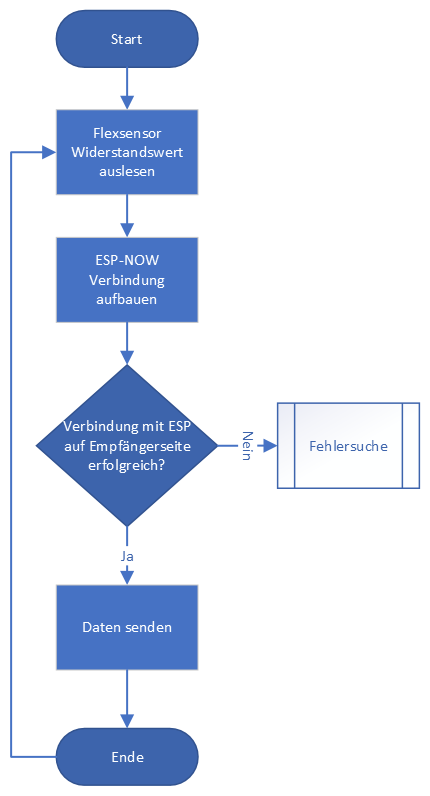
\includegraphics[width=0.8 \linewidth]{Flussdiagramm_Software_Handschuh}}
		%\caption*{Ladislaus Szabo}
	\end{center}
\end{figure}
\hfill \break
Der Code der Programmierung des ESP32 wurde in C/C++ geschrieben. Am Anfang werden die einzelnen Werte der Flexsensoren 
ausgelesen, die per Ansteuerung des Multiplexers und des danach sitzenden ADCs bestimmt werden. Die ESP-NOW Verbindung wird 
danach aufgebaut. Diese dient zur drahtlosen Datenübertragung. Wenn die Verbindung mit dem ESP32 der Empfängerseite erfolgreich 
war, dann werden die Daten an die Empfängerplatine (Roboterhand) gesendet. Falls dies allerdings nicht erfolgreich war, dann 
muss eine Fehlersuche durchgeführt werden. Ein oftmals auftretender Grund ist, dass die beiden ESPs zu weit auseinander liegen. 
Falls diese Schritte alle abgearbeitet wurden, dann geht das ganze Prozedere wieder von vorne los. \\
\\
\paragraph{Gliederung}
\hfill \break
\hfill \break
Am Anfang des Senderprogramms werden die zu inkludierenden Bibliotheken eingebunden. Diese beinhalten die I2C Kommunikation für 
den ADC, die Möglichkeit ESP-NOW zu verwenden, indem auch zusätzlich die Wifi Bibliothek inkludiert wird. \\
\\
Danach werden die ADC-Parameter festgelegt, sowie die Ports zur Ansteuerung des Multiplexers. Minimale und maximale 
Widerstandswerte werden festgelegt, damit es bei einer kleinen Toleranz im ganz unteren und oberen Bereich trotzdem immer den 
minimalen oder maximalen Wert erreicht. \\
\\
Die ESP-NOW Parameter sind noch zu definieren. Also die Empfänger-Adresse, die Nummer des Flexsensors, sowie der Wert. Außerdem 
wird eine Funktion erstellt, die später dazu verwendet wird, um zu überprüfen, ob die Empfängerplatine (Roboterarm) die Daten 
erfolgreich empfangen hat. \\
\\
Im Setup Teil werden anfangs die Ausgänge festgelegt, die für den ADC notwendig sind, sowie die SDA und SCL. Danach wird das 
ESP-NOW-Setup erstellt. In diesem Bereich werden alle notwendigen Schritte abgearbeitet, sodass man über ESP-NOW erfolgreich 
Daten senden kann. \\
\\
In der Loop wird dann der Multiplexer angesteuert und immer wieder aufsteigend durchgeschalten. Der Wert, der vom ADC, der
hinter den Multiplexer geschalten wurde, ausgegeben wird, wird dann durch eine Funktion in einen Wert umgerechnet. \\
\\
Dieser Wert wird dann in Form einer Zeichenkette, die im Format $"\$s:n:angepassterWert"$ geschrieben wird, an den ESP32 der 
Empfängerplatine gesendet (n…Eingang des Multiplexers 0 – 4; angepassterWert…ausgelesener Wert (liegt zwischen Minimum und 
Maximum, das oben festgelegt wurde)). Es wird dann noch im Serial Monitor ausgegeben, ob die Senderplatine (Handschuh) die 
Daten erfolgreich senden konnte oder nicht. \\
\\

\paragraph{Wichtige Codezeilen}
\hfill \break
\hfill \break
In dem obenstehenden Code kann man zwei erstellte integer Arrays sehen. Eines ist 
für das Speichern des minimalen Widerstandwertes zuständig. Dort werden dann die 
manuell gemessenen Werte eingetragen. Das Array besitzt fünf Variablen. Die Variable 
auf Stelle 0 des minWiderstand Arrays gibt den minimalen Wert des Daumens an. 1 gibt 
den jeweiligen für den Zeigefinger an, 2 gibt den jeweiligen für den Mittelfinger an, 
3 gibt den jeweiligen für den Ringfinger an und 4 gibt den jeweiligen für den 
kleinen Finger an. Somit kann jeder Finger im Array leicht einen neuen Wert 
zugewiesen bekommen und das Programm arbeitet automatisch mit den neu zugewiesenen 
Werten bei erneutem Hochladen auf den ESP32. \\
\\
Obenstehend ist nun der Codeabschnitt zu sehen, in welchem der vom ADC verarbeitete 
Wert des Flexsensors von dem ESP32 ausgelesen wird. Dieser wird dann mit dem Wert 
des minimalen und maximalen Widerstands verglichen. Wenn der ausgelesene Widerstandswert 
unter jenem des minimal erlaubten ist, dann wird dieser auf den minimal erlaubten 
gesetzt, um grobe Fehlmessungen zu vermeiden. Das gleiche gilt für den anderen Fall, 
nämlich, wenn der ausgelesene Wert über dem maximal festgelegten liegt. Dann wird 
der ausgelesene auf den maximal zulässigen Wert gesetzt. Dies ist sehr wichtig, da 
ein zu hoher Wert meist indiziert, dass es keine Verbindung zwischen dem Flexsensor 
und den anderen Komponenten, wie dem ADC, mehr besteht. Der Wert ist dann um ein 
Vielfaches höher als gewünscht. Um eine Beschädigung auf Empfängerseite, beziehungsweise 
dem dadurch folglich falschen Ansteuern der Servos zu verhindern, ist diese Maßnahme 
notwendig. Die Servos könnten sich ansonsten zu weit drehen und eine Beschädigung an 
der Mechanik hinterlassen. \\
\\
In obenstehendem Codeabschnitt wird der Multiplexer richtig eingestellt. Je nach 
Channelnummer wird dann festgelegt, welcher Eingang zum ADC weitergeschalten werden 
soll. Durch einige if-Bedingungen kann somit immer sichergestellt werden, dass man 
zu jeder Zeit den richtigen, gewünschten Wert auslesen kann. \\
\\
Untenstehend kann man noch anhand einer einfachen Logikschaltung eines 2-zu-1 
Multiplexers die Funktionsweise eines Multiplexers. Grundsätzlich wird über 
elektrische Signale einer von mehreren Eingangssignalen an den Ausgang 
durchgeschaltet. Meist funktioniert dies durch Halbleiterelemente. Das Steuersignals
schaltet noch zusätzlich. \\
\\
\begin{figure}[H]
	\begin{center}
		\scalebox{1.2}
		{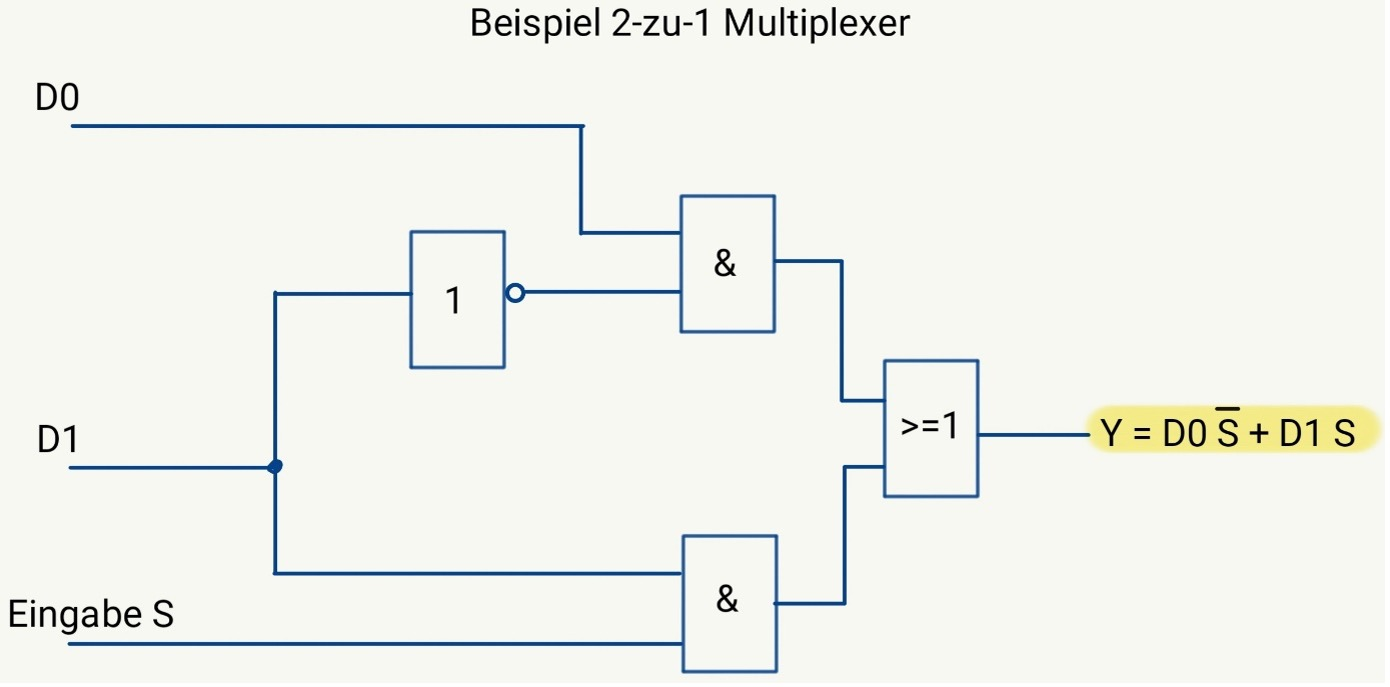
\includegraphics[width=0.8 \linewidth]{Multiplexer_Beispiel}}
		%\caption*{Ladislaus Szabo}
	\end{center}
\end{figure}
\hfill \break
Obenstehend sieht man nun das Format, in welchem die Daten an die Empfängerseite 
gesendet werden. Es wird ein String geformt. Dieser beginnt mit einem \$. Dies zeigt 
an, dass nun ein \"Befehl\" gesendet wird und man diesen verwerten soll. Danach noch 
ein \"s\" als Abkürzung für Servo. Der String von der Laufvariable \"i\" gibt dann an, 
welcher Wert nun gesendet wird, also beispielsweise \"\$s:1\" würde bedeuten, dass nun 
der Wert des Daumens gesendet wird. Der \":\" gibt dann eine Trennung an. Auf der 
Empfängerseite muss erkannt werden, wo die Trennung zwischen der Nummer des Fingers 
und des Wertes, zu dem sich der Servo dann hinbewegen soll, liegt. Der String von 
\"angepassterWert\" gibt dann den Wert an, den die Servoposition dann endgültig 
erreichen soll. Dabei ist es wichtig, dass dies allerdings auf der Empfängerseite 
dann umgesetzt wird. Auf der Senderseite wird der angepasste Wert zuvor 
möglicherweise durch die Grenzen von minimalem oder maximalem Widerstandswert 
begrenzt und dann noch mit der map-Funktion auf Werte von 0-100 gebracht, da damit 
dann auf der Empfängerseite gearbeitet wird. Gesamt schaut der String für den 
Zeigefinger mit dem angepassten Wert und einem halben Abknicken dieses also wie 
folgt aus: \"\$s:2:50\". Schlussendlich wird dann der gesamte String namens 
\"package\" per drahtloser Übertragung über ESP-NOW von der Sender- zu der 
Empfängerplatine gesendet. \\
\\



\subsection{Roboterhand}

\subsubsection{Grundlegende Vorraussetzungen}
Die Software des Roboterarmes ist dafür verantwortlich, dass die von der Handschuhplatine, via ESP32, gesendeten Daten 
erfolgreich empfangen und gespeichert werden. Die Software wird hierzu per UART-Schnittstelle auf den ESP32 hochgeladen. 
Die Daten der Flexsensoren, die man bereits erhalten hat, sollen dann verarbeitet werden. Anhand des Widerstandwertes und 
der jeweiligen Veränderung, wird dann der Winkel des Servos eingestellt. Eine Fehlerkorrektur soll sicherstellen, dass die 
Griffkraft passend eingestellt wird. Jeder Flexsensor hat unterschiedliche Widerstandswerte, es muss also über jeden Finger 
eine gezielte Software geschrieben werden, damit man schlussendlich durch das Zusammenspiel aller Finger die Griffkraft 
richtig einstellen kann. Falsche Messungen sollen bestmöglich korrigiert werden, sodass die Servos jeweils die richtigen 
Winkeleinstellungen erhalten. Der ESP32 stellt hierbei die Zentrale der Steuerung dar.

\subsubsection{Konzepte und Überlegungen \textcolor{red}{Fabian}}
Datenübertragung, Programmiersprache/Entwicklungsumgebung und Benutzerfreundlichkeit siehe 6.1.1! \\
\\
\paragraph{Testen}
\hfill \break
\hfill \break
Die von der Senderplatine (Handschuh) gesendeten Daten sollen ausgelesen werden. Sie wurden nach einem bestimmten Format 
(Schema) gesendet. Diese Daten sollen nun ausgewertet werden. Diese Daten werden nun dazu verwendet, um die einzelnen Servos 
anzusteuern. Dabei wird zuerst die Servo Nummer der empfangenen Daten ausgelesen und dann der Wert. Je nachdem wie groß der
Wert ist, dreht sich der Servo. Es kann dann getestet werden, ob sich der Servo tatsächlich dreht und somit, ob die 
Kommunikation mit dem Servo funktioniert. Wenn man die 3D-gedruckten Finger dann per Angelschnur mit den Servos verbindet, 
dann kann man am besten feststellen, ob die Software richtig läuft oder nicht. \\
\\
\paragraph{Allgemeines Konzept}
\hfill \break
\hfill \break
Die über ESP-NOW empfangenen Daten (Widerstandswerte samt Nummer des Flexsensors) sollen ausgelesen werden. Dadurch kann dann 
bestimmt werden, welcher Servo sich um wie viel drehen soll. Es muss festgestellt werden, dass die Daten über eine 
Datenkorrektur (Median der letzten 5 Werte) korrigiert wird. Das soll dazu beitragen, dass Fehlmessungen nicht in die Werte, 
die an die Servos übergeben werden, einfließen. Dadurch wird sichergestellt, dass die korrigierten Werte weniger anfällig für 
große Schwankungen gegenüber der möglicherweise fehlgemessenen Werten (Wackelkontakt zwischen Flexsensor und Sendeplatine) sind. 
Durch die Strommessung kann dann noch festgestellt werden, ob ein Finger blockiert. Dies ist dann der Fall, wenn der Strom zu 
lange einen gewissen festgelegten Schwellwert übersteigt. Die Servos sollen am Ende dann mit den korrigierten Werten angesteuert 
werden und sich ja nach Wert dann um eine einen bestimmten Winkel drehen, sodass der 3D-gedruckte Finger herangezogen oder
entlastet wird.
\\

\subsubsection{Realisierung und Gliederung \textcolor{red}{Fabian}}
\paragraph{Realisierung}
\hfill \break
\hfill \break
\begin{figure}[H]
	\begin{center}
		\scalebox{0.5}
		{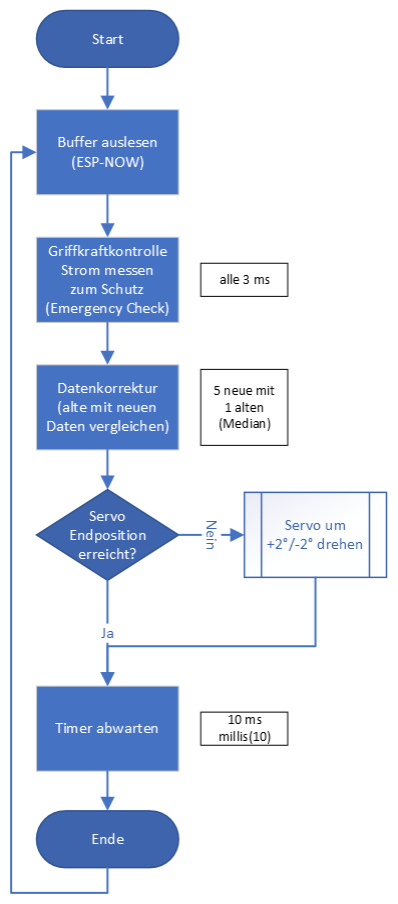
\includegraphics[width=0.8 \linewidth]{Flussdiagramm_Software_Roboterhand}}
		%\caption*{Ladislaus Szabo}
	\end{center}
\end{figure}
\hfill \break
Der Code der Programmierung des ESP32 wurde in C/C++ geschrieben. \\
Am Anfang wird der Buffer des ESP32 ausgelesen. Die von der Senderplatine (Handschuh) empfangenen Daten werden verarbeitet. 
Der Strom, der eine mögliche Blockierung eines Fingers erkennen kann, muss alle 3ms gemessen werden. Wenn dieser je Finger zu 
hoch ist, dann muss dieser Finger vorerst auf dem momentanen Wert belassen werden oder auf den maximalen Wert gesetzt werden. 
Dieser beschreibt die Stellung, wenn ein Finger nicht gebeugt wurde. Da die empfangenen Daten möglicherweise eine Fehlmessung 
beinhalten, muss eine Datenkorrektur diese entfernen. Der Median der letzten 5 Werte wird zu diesem Zweck verwendet. Dies soll 
dazu führen, dass ein Wert, der sehr anders als die weiteren 4 Werte ist, nicht an die Servos gesendet wird, sondern aussortiert 
wird. Nachdem dann alle Werte gesendet werden, wird überprüft, ob die Endposition des jeweiligen Servos erreicht wurde. Falls 
nein, dann darf sich der Servo weiter zu dem gesendeten Wert hinbewegen. Falls dann die gewünschte Endposition erreicht ist 
oder der Servo sich in eine beliebige Richtung dreht, dann wird noch der Timer von 10ms abgewartet und das Prozedere beginnt 
wieder von vorne.
\\
\begin{figure}[H]
	\centering
	\scalebox{1.5}{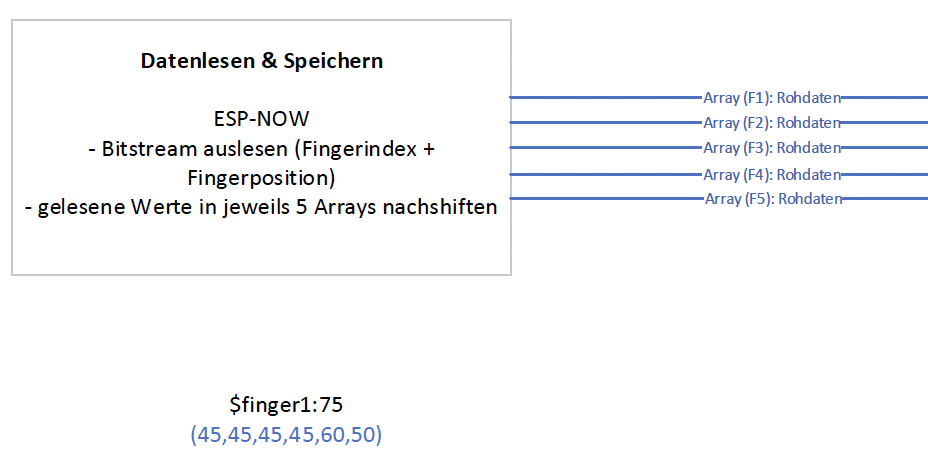
\includegraphics[width=0.8\linewidth, angle=-90]{Softwaremap_1}}
	%\caption*{Ladislaus Szabo}
\end{figure}
\begin{figure}[H]
	\centering
	\scalebox{1.8}{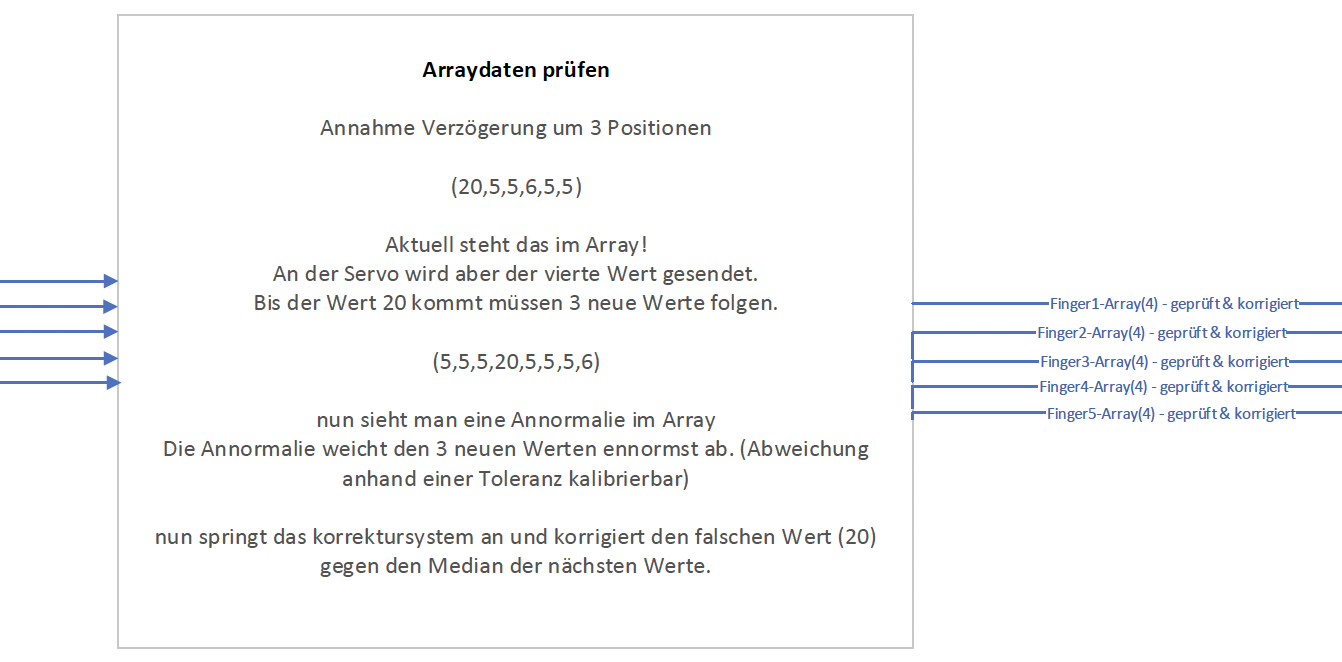
\includegraphics[width=0.8\linewidth, angle=-90]{Softwaremap_2}}
	%\caption*{Ladislaus Szabo}
\end{figure}
\begin{figure}[H]
	\centering
	\scalebox{1.1}{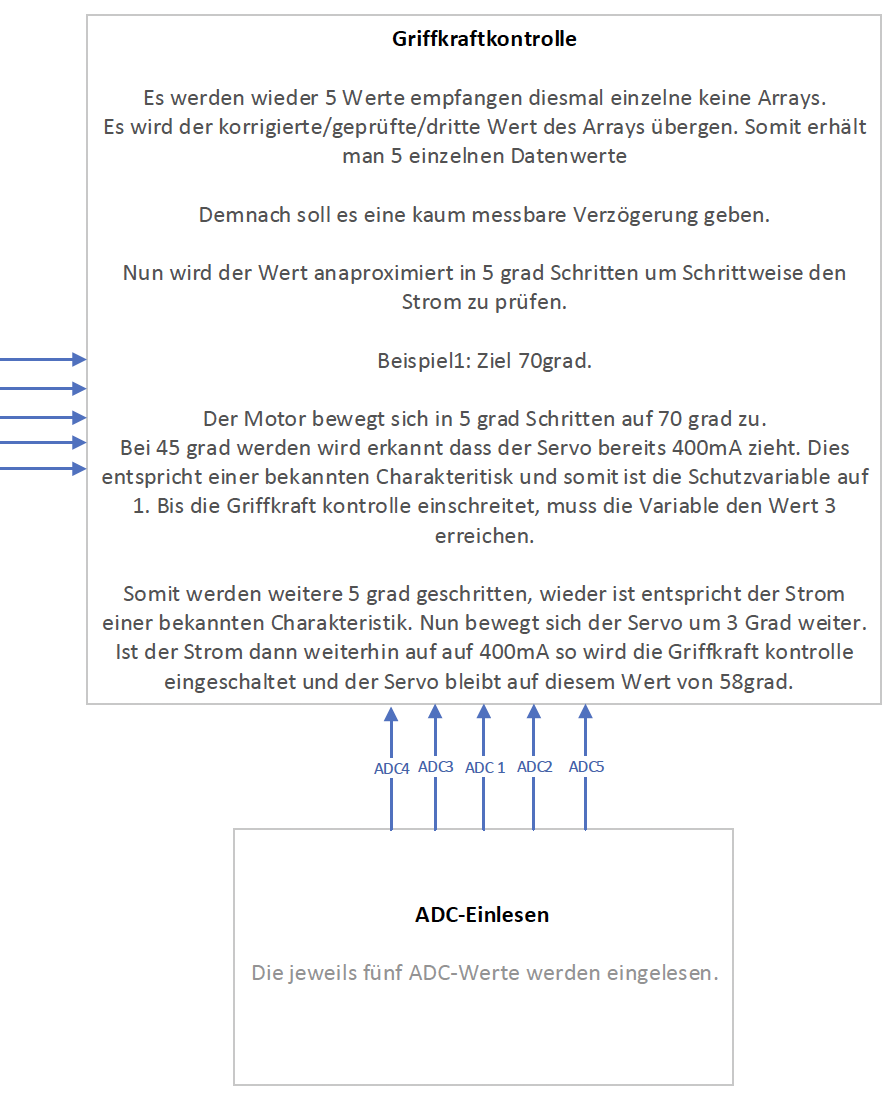
\includegraphics[width=0.8\linewidth, angle=-90]{Softwaremap_3}}
	%\caption*{Ladislaus Szabo}
\end{figure}
\hfill \break
Als Erstes werden die von der Senderplatine gesendeten Daten ausgelesen. Diese 
werden mit ESP-NOW übertragen. Gesendet wird in folgendem Format: 
\$fingerNummer:Wert. Somit kann herausgefunden werden, welcher Wert eines 
bestimmten Fingers gerade gesendet wird. Der Fingerindex (Nummer) gibt dabei den 
Finger des Handschuhs an. Die Fingerposition kann einen Wert von 0-100 
(Minimum-Maximum) annehmen. Die ausgelesenen Werte werden dann jeweils bei jedem 
neuen Auslesen um eine Stelle nach rechts geshiftet. Somit ergibt sich ein Array, 
das eine maximale Anzahl von 5 Werten pro Zeile erlaubt. Um zu vermeiden, dass 
sehr von den anderen Werten abweichende Zahlen in die Steuerung der Servos miteinfließen, 
wird der Median aus den 5 Werten des Arrays gebildet. Dabei würde dann beispielsweise 
ein Wert von 20, wenn sich die anderen 4 im Bereich zwischen 2 und 5 liegen, 
herausgefiltert werden, da dieser nicht in der (festlegbaren) Toleranz liegt. 
Der Median wird also im schlimmsten Fall zur Vermeidung von Fehlern verwendet. 
Die Griffkraftkontrolle achtet ständig auf den aktuellen Stromwert. Falls dieser 
zu hoch sein sollte, wird die Position des Servos gehalten. Die aktuellen Werte, 
beziehungsweise der Median im Falle einer Abweichung, werden übergeben. Der 
Servo wird dann jedes Mal um 5° weitergedreht. Die Schutzvariable hat dann anfangs 
den Wert 1, wenn allerdings der Strom laut Charakteristik einen bestimmten Schwellenwert 
überschreitet, dann wird die Schutzvariable auf den Wert 2 gesetzt und der Servo 
dreht sich nur noch um 3° weiter. Wenn schlussendlich dann der Strom zu hoch sein 
sollte, dann bleibt der Servo auf der momentanen Position stehen und die Schutzvariable 
wird auf den Wert 3 gesetzt. Damit soll eine mögliche Blockierung der Finger 
erkannt und die weitere Drehung des Servos erfolgreich gestoppt werden, um 
Schäden an der Mechanik zu vermeiden. \\
\\
\textbf{UART Funktionsweise}
\\
Der Arduino, beziehungsweise der ESP, werden über die serielle Verbindung UART 
(Universal Asynchronous Receiver and Transmitter) vom Computer angesprochen. 
Dabei stellt diese Verbindung eine asynchrone Datenübertragung mit fester Baudrate, 
Datenbits, Paritätsbits und Stoppbits dar. Es werden ausschließlich zwei Leitungen 
benötigt, nämlich eine zum Senden von Daten (TX – Transmit) und eine zum Empfangen 
von Daten (RX – Receive), um eine Möglichkeit der Kommunikation zu ermöglichen. 
Die Start- und Stopbits geben an, wann gesendet werden soll und wann dies nicht 
mehr geschehen soll. Sobald der Sender ein Startbit erhält, beginnt die Übertragung 
der Daten, aber beim Empfangen des Stopbit wird diese unterbrochen. Es wird 
dadurch keine Clock benötigt, da die Baud Rate dies regelt, allerdings ist zu 
beachten, dass diese maximal 10\% von jeder des anderen Geräts abweichen darf. 
Die Baud Rate gibt an, wie viele Symbole pro Sekunde übertragen werden. Dabei 
kann ein Symbol ein einzelnes Bit oder eine Gruppe von Bits sein. Die Baudrate 
gibt also an in welchem Abstand jeweils ein Symbol gesendet wird (1s/Baudrate) 
oder eben im Umkehrschluss auch, wie viele Symbole pro Sekunde gesendet werden 
(Baudrate/1s). \\
\\
\textbf{Beispiel Protokoll für 8-bit Packet} \\
Es ist ein Startbit vorhanden (LOW), dann noch 8 Datenbits (inklusive einem 
Paritybit, das Fehler identifizieren kann) und ein oder zwei Stopbits (HIGH). 
Zur Kontrolle, ob es eine gerade oder ungerade Anzahl von Highbits gibt, wird 
ein Paritybit mitgesendet, das angibt, ob die Anzahl dieser gerade oder ungerade 
ist. Es gibt klarerweise keine hundertprozentige Sicherheit, aber man kann sich 
mehr auf die Nutzbarkeit der Daten verlassen. Wenn das Paritybit auf 0 gesetzt 
ist (odd), dann ist die Anazhl der Highbits ungerade. Wenn das Paritybit auf 1 
gesetzt ist (even), dann ist die Anzahl der Highbits gerade. Es werden am 
Schluss meistens zwei Stopbits gesendet, um eine längere Ruhephase zu realisieren. 
Dies führt zu einer stabileren Synchronität und Erhöhung der Robustheit gegen 
Signalstörungen. Bei UART wird das LSB (least significant bit) immer ganz rechts 
in den Daten gefunden. Sollte das Paritybit nicht stimmen, dann wird vom 
Empfänger an den Sender eine Anfrage mit der Bitte um erneutes Senden gesendet, 
da der Datensatz nicht stimmt. \\

\textcolor{red}{https://edistechlab.com/wie-funktioniert-uart/?v=fa868488740a}

\begin{figure}[H]
	\begin{center}
		\scalebox{1.0}
		{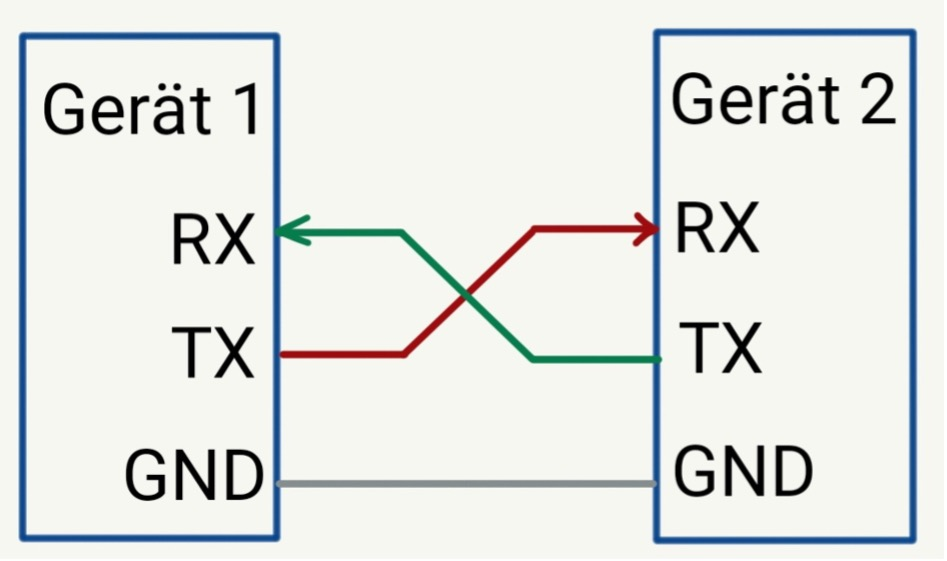
\includegraphics[width=0.8 \linewidth]{UART}}
		%\caption*{Ladislaus Szabo}
	\end{center}
\end{figure}
\hfill \break
\textbf{I2C Funktionsweise}
\\
I2C beschreibt eine Möglichkeit, über die zwei verschiedene Geräte miteinander 
kommunizieren können. Die Daten werden hintereinander gesendet und dies über zwei 
Leitungen. Es kann dabei mit bis zu 128 Teilnehmern kommuniziert werden. Am Ende 
interpretiert der I2C-Bus die Daten und steuert den Ablauf. Bei unserem Projekt ist 
der ESP32 der Master und die Flexsensoren beispielsweise die Slaves. Der Master ist 
dann der wichtige Bestandteil, da dieser für alle anderen Slaves derjenige ist, der 
sagt, was welches Bauteil machen soll. Dabei hängen alle Geräte beziehungsweise 
Bauteile an zwei Leitungen. Eine heißt SDA (serial data) und ist für die serielle 
Übertragung der Daten verantwortlich. Jedoch ist zu erwähnen, dass diese bidirektional 
benutzt wird. Das heißt es kann in beide Richtungen gesendet werden (Master zum 
Slave und umgekehrt). Es muss aber der Master regeln, also entweder Daten senden 
oder welche von einem Slave anfordern. Die zweite Leitung heißt SCL (serial clock) 
und ist für den Takt zuständig, der für alle per I2C verbundenen Geräte gilt. Es 
wird also ein synchroner Bus verwendet. \\
\\
\textbf{Beispiel Protokoll I2C}
Die Daten sind grundsätzlich in Datenpaketen verpackt, jedes besteht aus 1 Byte. 
Wenn nichts kommuniziert wird, dann hat SDA und SCL den Wert 1. Nachdem eine 
Start-Condition gesendet wurde, durch die alle Slaves wissen, dass sie nun auf den 
Master jederzeit reagieren sollen, wird die Adresse des Slaves gesendet, mit dem 
nun Daten ausgetauscht werden sollen. 7 Bit werden hierfür standardmäßig verwendet. 
Danach wird ein weiteres Bit gesetzt. Dieses kann den Wert 0, was Schreiben bedeutet, 
oder 1, was lesen bedeutet, haben. Nun ist der Slave an der Reihe. Dieser muss 
ebenso 0, wenn die Kommunikation bereitsteht, an den Master zurücksenden. Der Master 
sendet dann oder empfängt Daten vom Slave. Sobald alle Daten versendet wurden, 
kommt die Bestätigung. Der ganze Vorgang des Senden und Empfangens wird am Ende 
dann durch die Stop-Condition beendet. SDA wird hier auf 1 gesetzt, währenddessen 
SCL auch den Wert 1 besitzt. \\
\\
\textcolor{red}{http://fmh-studios.de/theorie/informationstechnik/i2c-bus/}
\\
\begin{figure}[H]
	\begin{center}
		\scalebox{1.2}
		{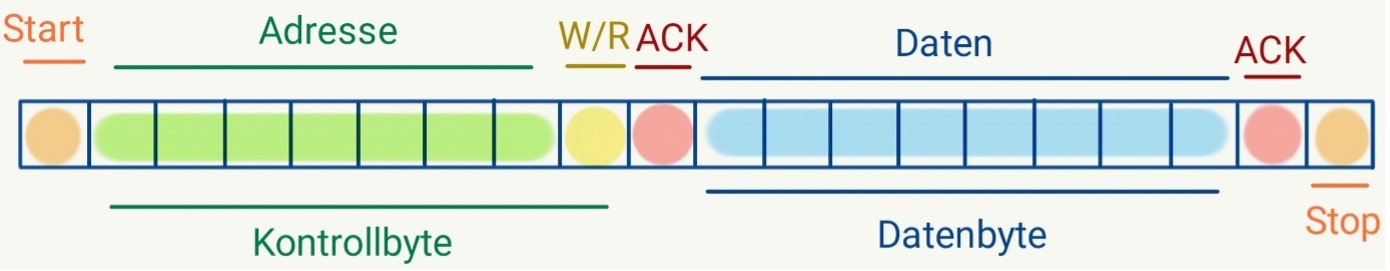
\includegraphics[width=0.8 \linewidth]{I2C}}
		%\caption*{Ladislaus Szabo}
	\end{center}
\end{figure}
\hfill \break


\subsection{User Interface}

\subsubsection{Grundlegende Vorraussetzungen}
Grundvorraussetzungen die das User-Interface erfüllen muss sind eine Anzeige der aktuellen Griffkraft in kg und eine Anzeige für
den aktuellen Winkel den jeder Servomotor zur Zeit hat. Es ist zwingend notwendig, dass für die Anbindung des GUIs keine technischen
Vorauskenntnisse benötigt werden. Der Verbindungsaufbau muss daher ebenfalls fast von selbst erfolgen. Multiplatform Kompatibilibtät
und eine stabile Laufleistung sollten ebenfalls gegeben sein, um dem Endbenutzer keine Technologie aufzuzwingen, die nicht gewünscht ist.

\subsubsection{Entwicklungsumgebung \textcolor{red}{Laci}}

Entschieden haben wir uns für QT. Dies ist eine C++ Entwicklungsumgebungen, die besonders Plattform unabhängig ist. Es sind keine Änderungen
des Queellcodes notwendig, um die Anwedung für MAC, LINUX oder WINDOWS kompatibel zu machen. Dies bezeichnet man auch als source 
code portability. Ebenfalls ist es relativ einfach möglich QML-Interfaces zu erstellen und diese mit umfangreichen Funktionalitäten auszustatten. \\
\\ 
Weitere Eigenschaften von Qt sind:
\begin{itemize}
	\item ein GUI-Designer
	\item ein Debugger
	\item eine 3D-Umgebung um Modelle zu animieren
\end{itemize}

\subsubsection{Konzepte und Überlegungen \textcolor{red}{Laci}}

\paragraph{Allgemeines Konzept}
\hfill \break
\hfill \break
Zunächst musste überlegt werden, wie die grafische Oberfläche aussehen soll. Diese wird nämlich immer vor allen Funktionalitäten 
erstellt, um die anschließende Programmierung übersichtlicher und gegliedert durchführen zu können. Das grafische Interface wurde 
in der Beschreibungssprache QML erstellt, welche vielseitige Möglichkeiten zur individuellen Gestaltung bietet. Das Erstkonzept
sieht folgendermaßen aus:
	\begin{figure}[H]
		\begin{center}
			\scalebox{1.2}
			{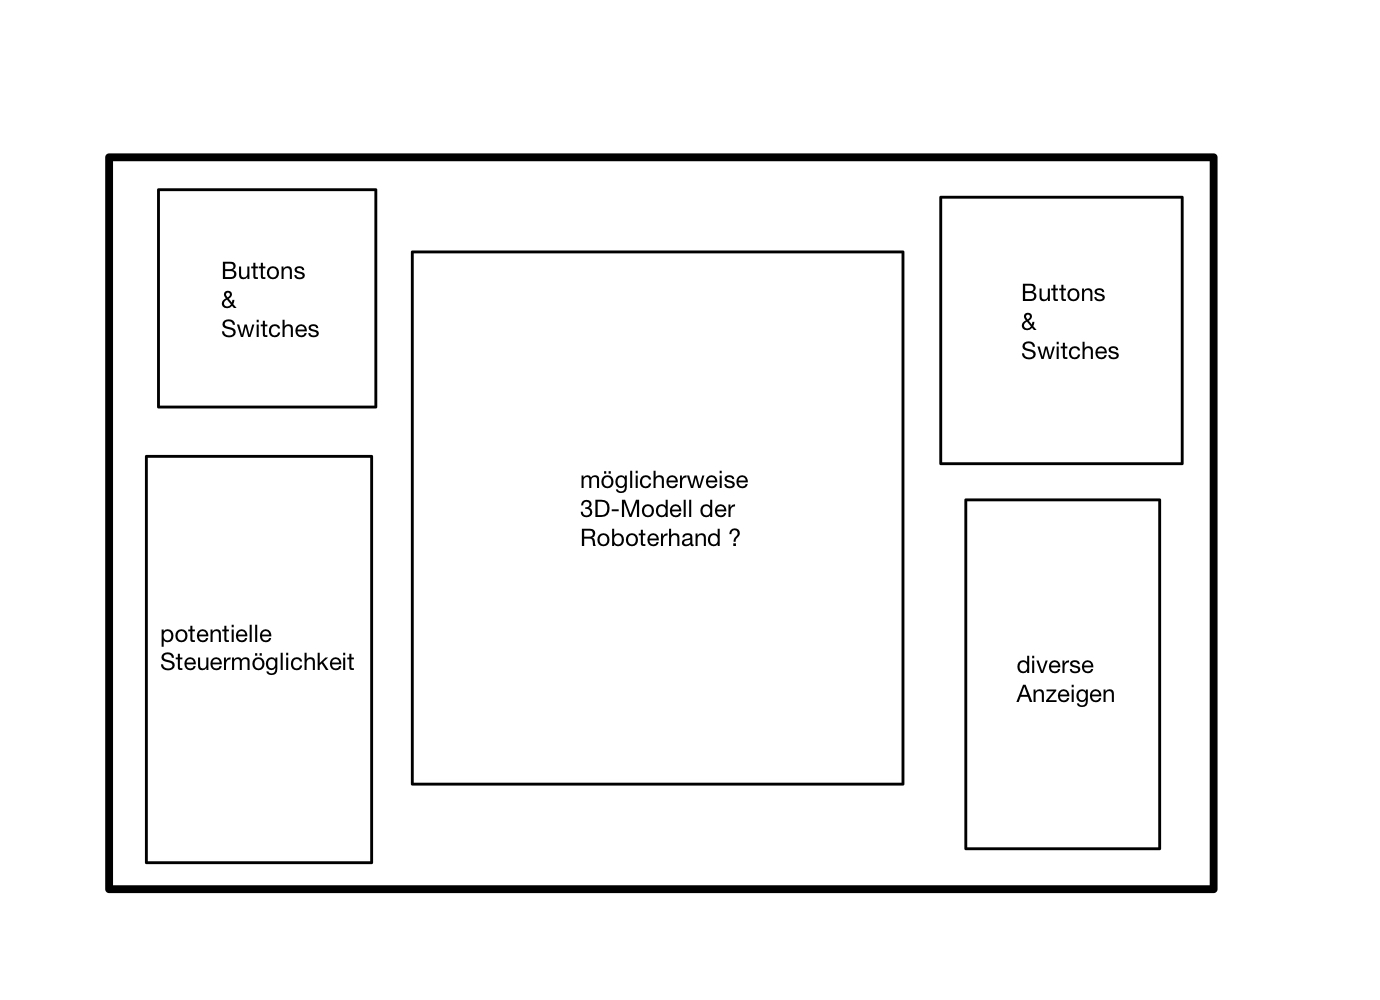
\includegraphics[width=0.8 \linewidth]{Konzept_UserInterface}}
			%\caption*{Ladislaus Szabo}
		\end{center}
	\end{figure}
Zu sehen sind die ersten Überlegungen bezüglich des visuellen Layouts. Auf der rechten Seite des Bildschirms sollen die erforderlichen
Anzeigen für die Parameter der Griffkraft und des Servodrehwinkels abgebildet werden. Links und rechts oben sollen diverse Knöpfe 
und Schieberegler zur weiteren Navigation und Kontrolle des UIs platziert werden. Optional kann noch ein 3D-Modell und Regler für 
die externe Steuerung der Roboterhand hinzugefügt werden. Diese Features sind allerdings nicht gefordert. \\
\\


\subsubsection{Realisierung und Gliederung \textcolor{red}{Laci}}

%--------------------------------------------------------------------------
%--------------------------------------------------------------------------
%==TESTS-UND-MESSUNGEN=====================================================
\section{Tests und Messungen}
\subsection{\textcolor{purple}{Platzhalter für diverse Unterpunkte}}

%--------------------------------------------------------------------------
%--------------------------------------------------------------------------
%==PROJEKTMANAGEMENT=======================================================
\section{Projektmanagement}
\subsection{Projektstrukturplan}
\subsection{Milestoneplan}
Lastenheft fertig – 10.10.2023 \\
Kostenkalkulationen fertig – 24.10.2023 \\
Prototypen proof of concept –21.11.2023 \\
Hardwaredesign fertig – 05.12.2023 \\
PCB-Design fertig – 09.01.2024 \\
Softwareimplementierung für Integrationstest fertig - 30.01.2024 \\
Integration aller Komponenten – 06.02.2024 \\
User Interface fertiggestellt – 13.02.2024 \\
Abnahme durch die Projektbetreuer – 12.03.2024

\subsection{Gantt-Diagram}
\subsection{Meeting Struktur}

%--------------------------------------------------------------------------
%--------------------------------------------------------------------------
%==FERTIGUNGSUNTERLAGEN====================================================
\section{Fertigungsunterlagen}
\subsection{Mechanik}
\subsubsection{händische Skizzen}
\subsubsection{CAD-Zeichnungen}
\subsubsection{3D-Modelle}

\subsection{Hardware}
\subsubsection{Stromlaufpläne}
\subsubsection{Platinen}
\subsubsection{Bestückungslisten}

\subsection{Software}
\subsubsection{Diagramme}
\subsubsection{Code}

%--------------------------------------------------------------------------
%--------------------------------------------------------------------------
%==ERGEBNISSE-UND-ERKENNTNISSE=============================================
\section{Ergebnisse und Erkenntisse}

%--------------------------------------------------------------------------
%--------------------------------------------------------------------------
%==AUSBLICK================================================================
\section{Ausblick}

%--------------------------------------------------------------------------
%--------------------------------------------------------------------------
%==VERZEICHNISSE===========================================================
\section{Verzeichnisse}
\subsection{Quellenverzeichnisse}

\subsection{Abbildungsverzeichnis}
\subsection{Abkürzungsverzeichnis}

%--------------------------------------------------------------------------
%--------------------------------------------------------------------------
%==ANHANG==================================================================
\section{Anhang}


%--------------------------------------------------------------------------
%--------------------------------------------------------------------------
\end{document}